\documentclass[conference]{IEEEtran}
\IEEEoverridecommandlockouts
% The preceding line is only needed to identify funding in the first footnote. If that is unneeded, please comment it out.
\usepackage{cite}
\usepackage{amsmath,amssymb,amsfonts}
\usepackage{algorithmic}
\usepackage{graphicx}
\usepackage{textcomp}
\usepackage{xcolor}
\def\BibTeX{{\rm B\kern-.05em{\sc i\kern-.025em b}\kern-.08em
    T\kern-.1667em\lower.7ex\hbox{E}\kern-.125emX}}

\usepackage{url}
\usepackage{hhline}
\usepackage{booktabs}
\usepackage{multirow}
\usepackage{subfigure}
\usepackage[linesnumbered,boxed,ruled,commentsnumbered]{algorithm2e}
\newcommand{\figref}[1]{Figure \ref{#1}}
\newcommand{\eqnref}[1]{Eq. \ref{#1}}
\newcommand{\tabref}[1]{Table \ref{#1}}
\newcommand{\secref}[1]{Section \ref{#1}}
\newcommand{\algoref}[1]{Algorithm \ref{#1}}
\usepackage{color}
\newcommand{\KZ}[1]{\textcolor{red}{Kenny: #1}}
\newcommand{\YZ}[1]{\textcolor{green}{Yizhu: #1}}

\begin{document}

\title{DDRel: A new dataset for interpersonal relation classification in dyadic dialogues\\
%{\footnotesize \textsuperscript{*}Note: Sub-titles are not captured in Xplore and
%should not be used}
\thanks{Identify applicable funding agency here. If none, delete this.}
}

%\author{ \IEEEauthorblockN{Qi Jia$^1$ \hspace*{1cm}
%	Hongru Huang$^2$ \hspace*{1cm}
%	Kenny Q. Zhu$^3$ \thanks{\hspace{2mm}The corresponding author.}}
%	\IEEEauthorblockA{\texit{Shanghai Jiao Tong University} \\
%	Shanghai, China \\
%	\texttt{\{$^1$Jia\_qi,$^2$onedesire\}@sjtu.edu.cn} 
%	\texttt{$^4$kzhu@cs.sjtu.edu.cn} }	
%}
\author{\IEEEauthorblockN{1\textsuperscript{st} Given Name Surname}
	\IEEEauthorblockA{\textit{dept. name of organization (of Aff.)} \\
		\textit{name of organization (of Aff.)}\\
		City, Country \\
		email address or ORCID}
	\and
	\IEEEauthorblockN{2\textsuperscript{nd} Given Name Surname}
	\IEEEauthorblockA{\textit{dept. name of organization (of Aff.)} \\
		\textit{name of organization (of Aff.)}\\
		City, Country \\
		email address or ORCID}
	\and
	\IEEEauthorblockN{3\textsuperscript{rd} Given Name Surname}
	\IEEEauthorblockA{\textit{dept. name of organization (of Aff.)} \\
		\textit{name of organization (of Aff.)}\\
		City, Country \\
		email address or ORCID}
	\and
	\IEEEauthorblockN{4\textsuperscript{th} Given Name Surname}
	\IEEEauthorblockA{\textit{dept. name of organization (of Aff.)} \\
		\textit{name of organization (of Aff.)}\\
		City, Country \\
		email address or ORCID}
	\and
	\IEEEauthorblockN{5\textsuperscript{th} Given Name Surname}
	\IEEEauthorblockA{\textit{dept. name of organization (of Aff.)} \\
		\textit{name of organization (of Aff.)}\\
		City, Country \\
		email address or ORCID}
	\and
	\IEEEauthorblockN{6\textsuperscript{th} Given Name Surname}
	\IEEEauthorblockA{\textit{dept. name of organization (of Aff.)} \\
		\textit{name of organization (of Aff.)}\\
		City, Country \\
		email address or ORCID}
}


\maketitle

\begin{abstract}
Interpersonal language style shifting in dialogues is an interesting and almost instinctive ability of humans. Understanding interpersonal relationship from language content is also a crucial step toward further understanding dialogues. 
Previous work mainly focuses on relation extraction between 
named entities in texts.  In this paper, we propose the task of 
relation classification of interlocutors based on their dialogues.  
We crawled movie scripts from IMSDb, and annotated the relation labels for each session according to 13 pre-defined relationships. 
The annotated dataset DDRel consists of 6300 dyadic dialogues sessions 
between 694 pairs of speakers with 53,126 utterances in total. 
We also construct session-level and pair-level relation classification tasks with widely-accepted baselines. The experimental results show that 
this task is challenging for existing models and the dataset will be useful 
for future research.
\end{abstract}
%\IEEEraisesectionheading{
% %\IEEEraisesectionheading{
% %\IEEEraisesectionheading{
% \input{intro}
\section{Introduction}\label{sec:intro}
 %}
% \section{Introduction}\label{sec:intro}

% \begin{enumerate}
% \item Motivation: application scenarios (with 1-2 running examples);
% \item Characteristics of the data sources and their challenges;
% \item Briefly introduce previous approaches to extract information 
% from images including setting the document zone, and their limitations.
% \item General flow of our approach (may give a diagram here)
% \end{enumerate}
% scenary

Due to ever evolving hardware and software, many medical images
such as electro-cardio graphs (ECGs), X-ray or ultrasound images  
are directly printed and stored in hard copy formats. 
% \KZ{Insert 4 example images here.}
%Examples are shown in \figref{fig:medicalImages}. 
% These images often contain a mix of graphics and text, which
% include parameter settings of the hardware, test measurements or simple
% diagnosis. 
These images often contain a mix of graphics and text, which 
include technical settings of the hardware used, test measurements or simple diagnoses.
Recently, there has been a growing demand for digitizing such 
medical information from paper media sources, especially legacy ones, or patients who want to keep track of these documents by themselves digitally. 
Apart from scanning the graphics into a digital format, extracting 
the semi-structured textual information is also an important part of
building electronic medical records for patients. 

%\begin{figure}[!htb]
%\centering
%\subfloat[ECG]{
%\label{fig:medicalimage:ecg}
%\epsfig{file=figure/17_ori.eps, width=0.4\columnwidth}
%}
%% \hfill
%\subfloat[MRI]{
%	\label{fig:medicalimage:mrt}
%	\epsfig{file=figure/MRI.eps, width=0.4\columnwidth}
%}
%\\
%\subfloat[X-RAY]{
%\label{fig:medicalimage:xray}
%\epsfig{file=figure/X-RAY.eps, width=0.4\columnwidth}
%}
%%\hfill
%\subfloat[EEG]{
%\label{fig:medicalimage:eeg}
%\epsfig{file=figure/EEG.eps, width=0.4\columnwidth}
%}
%\caption{Examples of Medical Images}
%\label{fig:medicalImages}
%\end{figure}

Optical character recognition (OCR)  \cite{mori1992historical,smith2007overview} is 
a traditional technique used to turn images of printed text into machine encoded
text. It is well researched and performs well on plain text 
documents such as novels and reports, for a variety of languages. 
%For example, Tesseract, which is one of 
%the most popular open source multilingual recognizers, logs an error 
%rate of 3.72\% for English words and 3.77\% for simplified 
%Chinese characters\cite{smith2009adapting}. 
%Google Books \cite{googlebooks} and Gutenberg \cite{gutenberg} are
%projects which have scanned a large number of paper books into text for free and open
%access. These projects made exclusive use of OCR for this conversion and 
%achieved high accuracy \cite{vincent2007google} \cite{lebert2008project}. 
% 99\% for Gutenberg project \cite{lebert2008project}. 
% \KZ{Give the accuracy of google and gutenberg if available.}


\begin{figure}[th]
\centering
\epsfig{file=figure/17_b.eps, width=0.8\columnwidth}
\caption{An ECG image with text area (red circle) of interest.}
\label{fig:ecgexample2}
\end{figure}

For a semi-structured medical image, such as 
\figref{fig:ecgexample2}, we would like to extract the attribute-value 
pairs (e.g., {\em Vent. rate = 63 bpm}) and possibly other values such as
date ({\em 18-Nov-2010}) and time ({\em 9:13:02}) since those values endow us with lots of information about the patient. 
Existing OCR software cannot extract such structured information in a straightforward 
fashion, 
but instead it produces rather convoluted results from the whole image, 
similar to those in \figref{fig:ocrre}, which was produced by Tesseract, 
a popular multi-lingual recognizers. 
% \KZ{Maybe include the x-y coordinate info in the output as well?}  

\begin{figure}[th]
\centering
\scriptsize
\begin{verbatim}
<p class="ocr_par" title="box 263 33 444 119">
   <span class="ocr_l" title="box 264 33 336 45">
       <span class="ocrx_w" title="box 264 33 299 45">Vcnt.</span> 
       <span class="ocrx_w" title="box 308 34 336 45">rule</span> 
   </span>
   <span class='ocr_l'>
       <span class="ocrx_w" title="box 264 51 283 64">PR</span> 
       <span class="ocrx_w" title="box 291 51 346 64">Interval</span> 
       <span class="ocrx_w" title="box 389 52 411 64">140</span> 
       <span class="ocrx_w" title="box 420 55 439 64">ms</span> 
   </span>
   ...
   </span>
</p>
<p class="ocr_p" dir="ltr">
   <span class="ocr_l">
       <span class="ocrx_w" title="box 396 33 411 45">53</span> 
       <span class="ocrx_w" title="box 420 33 449 48">bpm</span> 
   </span>
</p>
\end{verbatim}
\caption{Snippet OCR results in XML, input to our framework.}
\label{fig:ocrre}
\end{figure}


%\input{xmlre1}

%However, OCR alone does not work well on semi-structured text and hence
%can't be directly used for information extraction from the aforementioned
%medical images. \KZ{Give the reason here, perhaps because OCR models are
%largely Markov based? So semi-structured data breaks the flow of text.}
%When a medical image is input to an ordinary OCR software, the spatial 
%information of the text components is often lost or mixed with noises
%and errors.
%%The reason is OCR converts the whole images into text data, in which 
%%useful information often mix with noises and errors. 
%In this paper, we would like to extract the attribute-value pairs
%and possibly other values from \figref{fig:ecgexample1} 
%and \figref{fig:ecgexample2}. 
%% or medical ultrasonography report. 
%Such images contain lots of non-textual information or noises.

% example & ref
%\begin{figure}[ht]
%\centering
%\epsfig{file=figure/46.eps, width=0.8\columnwidth}
%\caption{ECG Images From Printer1}
%\label{fig:ecgexample1}
%\end{figure}

% \begin{figure}[ht]
% \centering
% \subfloat[Printer1]{
% \label{fig:ecgexample:a}
% \epsfig{file=figure/46.eps, width=0.48\columnwidth}
% }
% \hfill
% \subfloat[Printer2]{
% \label{fig:ecgexample:b}
% \epsfig{file=figure/17.eps, width=0.48\columnwidth}
% }
% \caption{ECG images from two different printers}
% \label{fig:ecgexample}
% \end{figure}

Also, errors in the OCR text \cite{darwish2007error,taghva1996evaluation} will greatly affect the effectiveness 
of other related tasks. Much work has been done to improve the performance of the OCR\cite{kolak2003generative,cesarini1998informys}. However, there are still a number of significant challenges involved in extracting the information from medical images or OCR results in XML form. 

% First, medical images differ from pure text document in that them have 
% layout information. 
First, medical images differ from pure text documents in that 
they contain layout information.
Although most current OCR engines attempt to reproduce the physical 
layout of the text units, 
%(along with X-Y coordinates) and store them 
%in a special format such as XML 
% (\KZ{Better in the previous example})
such spatial
information is approximate and sometimes inaccurate, which is why neighboring
text blocks in \figref{fig:ecgexample2}, such as ``Vent. Rate'' and
``63 bpm'' were not automatically combined into the same XML block, but were 
rather far apart (shown in two different ``classes'') in \figref{fig:ocrre} made by OCR softwares. 
%Even for images produced by the same ECG printer, 
%the XML results can still be very different as 
The spatial layout is sensitive to many factors, such as accidental spots 
on the prints, color and contrast, or the angle of the camera. 
%In this case, solutions for other application domains, for example, the web, 
%are not well suited for information extraction from printed documents \cite{bartoli2014semisupervised}. With such inaccurate
%layout information produced by OCR,
%it is not easy to write a simple wrapper program to extract useful
%data from images, even if the images come from the same printer. 

%Writing a wrapper for each
%individual image would be tedious and counter-productive. Therefore,
%a mechanism that makes use of the spatial locality of the 
%text units in the image and 
%accommodates slight variations in the spatial layout would make the extraction
%more accurate and fault-tolerant.

%For example, \figref{fig:ocrre} is the simplified OCR results for the ECGs in 
%\figref{fig:ecgexample1} and \figref{fig:ecgexample2}. The results are in the XML format and have attritube named {\em class} 
%for layout information. Although these two images share similar format. 
%OCR engine generates different results in that it splits elements that 
%should be in the same line into two lines in the second example. 
%XML is sensitive to the layout results so it's hard to tolerate 
%all the layout results. 
%
% example check the term
% layout of ocr results can be restore, so why OCR engine don't restore the results 
% using the similar methods as we do?
% or the way we handle the layout problem is quite simple

% Delete for TIP
% Second, exiting OCR engines make heavy use of Markov properties such as n-grams
% since they primarily target the transformation of large body of text 
% \cite{kolak2003generative}. 
% % \KZ{Needs some refs here.}
% Unfortunately, the semi-structured texts in medical images are often 
% short and not even written in complete sentences, thus breaking Markov assumption. To make
% matters worse, medical images contain scientific language, which may be
% very different from the training corpora of these OCR engines.
% This explains why we see errors like ``Vcnt'' and ``rule'' 
% in \figref{fig:ocrre}. 
% %can't guarantee a perfect performance, which means 
% %there are errors and noises in the OCR results.
% %Many of them due to the fact that the data are no longer long, continous
% %sentences, thus breaking the Markov assumption made by many OCR algorithms. 
% %In \figref{fig:ocrresub:b}, ``Vent." is misrecognized as ``Vcnt.". 
% Without sufficient contextual information, OCR may also misrecognize a 
% digit as an alphabetic character, or as another similar digit. 
% Furthermore, the mix of text with images and formatting
% lines often confuses the OCR engine, which is more biased toward full
% text images.
% Exact pattern matching, as used in
% traditional information extraction, doesn't work with such noisy OCR output
% as it doesn't tolerate noises or errors in text. 
% %It's hard to autocorrect these errors 
% %because image quality is the most important affecting factor. 
% %The text we are processing can be full of no meaning words or 
% %strange numbers. 
% A fuzzy matching strategy is more desirable in this case. 
% % example, what are the traditional IEs

Second, there are many types of medical images, resulting from a variety of
medical tests. Different equipments for the same test can produce vastly 
different images. Writing individual extraction wrappers 
for the OCR outputs of all these formats is tedious and inefficient, 
and difficult for non-programmers.
%not to mention that there are significant programming barriers for 
%writing these wrappers, especially for the medical professionals who are the
%end users of these extraction results. 
%A more user-friendly approach enabling users to specify such extraction requirements would be preferred. 
%There are various kinds of medical images, such as electrocardiograph report, 
%medical ultrasonography report, etc. 
%However the basic measures for each type of medical test (e.g., ECG), 
%are very similar from machine to machine. Only the layouts are 
%different. 
% example medical images

Finally, most off-the-shelf OCR programs are pre-trained with specific 
recognition models, which may not be suitable for the extraction of 
%medical images.
%Furthermore, changes in imaging equipment technology over time may produce 
%different formats, layout, or terminology, rendering existing OCR models 
%obsolete. 
Re-training the models requires a large amount of labeled data, which may
not be available. 
%Incremental training as more labeled data arrives
%is currently not supported by any OCR product.    

%There have been some limited attempts to address some of the above challenges. 
%One solution is a plugin of an OCR program that allows the user to specify 
%target zones of interest in the image to be extracted. The zones specified for
%one image can be applied to images with slight variations by adjusting against
%a fixed reference point that is supposed to exist in all these images.
%% \KZ{I think the problem is not so much with the zones, because we also
%% have zones, but rather with the reference point.}
%% \JY{}
%% example products
%% http://www.square-9.com/automated-data-extraction-optical-character-recognition
%The problem with this solution is its high reliance on the OCR zones  
%established by the user. The performance of the results is affected by the 
%accuracy of the zones. If the zones are too big, the results will be full of 
%noise. If the zones are too small, results will miss something. 
%
%Another solution involves using the page layout analysis technique. The page layout 
%analysis technique is used to determine where the text 
%resides on a page \cite{o1993document}, 
%% \KZ{This page layout analysis approach is not clearly described. I don't understand after reading this paragraph.}
%% By using page layout analysis technique, the hierarchy of physical components 
%% can be generated and to match with the hierarchy of logical components, which 
%% is predefined. 
%this includes identifying and categorizing the 
%regions of interest in the scanned image of a text document. 
%Typically, the first step is to segment text zones from 
%non-textual zones and arrange them in their original order. 
%Then in order to analyze the logical roles of the text zones 
%(titles, captions, footnotes, etc.), logical layout analysis 
%is used for labeling the semantics of the text zones.
%Generally, page layout analysis is used for documents. The problem with applying 
%such a technique on medical images is that it creates so much noises 
%that performance is ultimately affected. 
%For medical imaging reports like ECG, useful information is often 
%found in the small components of the image, while most of the images are 
%read as noises. 
% check paper and more description, weakness, ref

%In this paper, 
%we propose a spatial data description language, which borrows its syntax from
%PADS \cite{fisher+:pads}, an ad hoc data processing language, 
%for describing semi-structured data in medical images. 
%% ref
%We call this language OCR description language, or ODL. 
%ODL is designed for extracting and parsing semi-structured text data 
%from images. We believe that  information extraction from those data in ODL form may be much easier than extracting information from rough data or data in XML form, which means that our preprocessing part proves to be necessary.
%%An example ODL description for the image in 
%%\figref{fig:ecgexample2} is shown in 
%%\figref{fig:description}. \KZ{Make this description two column, and give
%%some brief explanation of this description here.} 
%%The parsing result of this description is shown
%%in \figref{fig:parsing result}. \KZ{Give some explanation of the results,
%%otherwise don't show the result here. E.g., you need to explain what F, E, etc.
%%mean. You want to say that even though rate has been recognized as rule,
%%the bpm value was still extracted (but still wrong!).}
%% \KZ{I removed the preprocessing part, cos it's not important. Talk about it in
%% discussion sec.}
%%The our approach starts by preprocessing the images for text results.
%To use this framework, the user first describes the components in the image
%that he or she is interested in extracting. This includes constant strings
%and variables of different data types.   
%ODL allows the user to specify the approximate spatial layout and constraints on
%the data, e.g., integers within 
%a certain range, real numbers with certain decimal points, etc. 
%%This information is then as the key component in our fuzzy matching strategy. 
%The system then automatically generates a parser for these medical images.
%This parser uses the output XML from OCR with spatial information as an input, 
%and outputs a data structure with values extracted for each variables
%in the description, unless there is an unrecoverable error during the parsing process.
%In addition, approximate layout information and constraints are used in parsing process 
%to tolerate noises and small format variations in the input images. 
%%Specifically, this method could be called fuzzy matching, meaning that more candidates could be saved after the parsing process.  It's obvious that we may have a higher probability to obtain the accurate result if more candidates are kept so that fuzzy match should be used properly in our system.
%%An autogenerated parser based on the ODL description can release us from 
%%repetitive work. In this way, we turn the task of writing complex parsers 
%%into describing information on images.
%
%
%When users process many images of the same format, the system 
%automatically discovers parsing errors given the current model and 
%prompts the user to manually correct some of the frequent and prominent
%errors, which effectively serves as an online labeling function. 
%These incrementally labeled data are then used to update the parsing model. 


%It should be emphasized that the incremental learning model is very important in our whole system. Incremental learning is a machine learning paradigm where the learning process takes place whenever we have new examples or data added to our baisc data set, leading to a most striking difference between incremental learning and traditional machine learning: it does not assume the availability of a sufficient training set before the learning process. What incremental learning in our system is really impressive: it does not require a relatively good and stable training set at first time. In fact, it could improve the parsing result with even relatively rough training sets at first by absorbing new data or corrective information as time passes in dynamic systems. Besides, the process would be very effective when there are some new images coming in since training process would not learn from scratch, which might waste time and computation resource.

%At last, we propose an incrementally human correction framwork which can 
%make the best use of human correction to handle the misrecognition problem. 
% Base on our experiments on about 500 real life ECG images, 
% our approach achieves p1 and p2 after p3 times human correction. 
% experimental results

% \begin{figure}[h]
% \begin{lstlisting}
% Oenum str_month_t{
% 	"Jan", "Feb", "Mar", "Apr",
% 	"May", "Jun", "Jul", "Aug",
% 	"Sept", "Oct", "Nov", "Dec"
% };

% Ounion month_t{
% 	Oint(1,12)	num;
% 	str_month_t	str;
% };

% Ostruct time_t{
% 	Oint(1,31)	day;
% 	"-";
% 	month_t	month;
% 	"-";
% 	Oint	year;
% };

% Ostruct triple_t{
% 	"Vent.";
% 	hskip(\s)	skip1;
% 	"rate";
% 	Oint x;
% 	"bpm";
% 	vskip(\n)	skip2;
% };

% Oscource Ostruct entry_t{
% 	time_t(<-,-,-,0.3l>) t;
% 	triple_t(<0.1w,-,0.5w,->) d;
% };
% \end{lstlisting}
% \caption{Description}\label{fig:description}
% \end{figure}


In order to solve above problems, We design a system which makes three main contributions:
\begin{enumerate}
\item Based on some previous work on data description language \cite{lamport1986document,taft1999post,fisher+:pads},we design a new declarative spatial data description language called \textit{OCR description language}, or ODL,
which allows users to specify spatial and data constraints in medical 
images(\secref{sec:syntax});
\item We propose a noise-tolerant parser which takes OCR results
the ODL description as input and outputs a data structure with values 
extracted for each variables in the description (\secref{sec:semantics});
\item We propose an incremental manual correction 
framework\cite{von2008recaptcha,zhu2012learnpads++}, which 
takes advantage of user corrections  and improves the productivity
significantly (\secref{sec:correction}).
%To be more specific, the framework improves the traditional machine learning methods by using a incremental learning process to avoid starting from scratch when we are trying to apply human corrections in the system. That means the framework would be more effective than most corrective systems.
\end{enumerate}


\section{Introduction}\label{sec:intro}
 %}
% \section{Introduction}\label{sec:intro}

% \begin{enumerate}
% \item Motivation: application scenarios (with 1-2 running examples);
% \item Characteristics of the data sources and their challenges;
% \item Briefly introduce previous approaches to extract information 
% from images including setting the document zone, and their limitations.
% \item General flow of our approach (may give a diagram here)
% \end{enumerate}
% scenary

Due to ever evolving hardware and software, many medical images
such as electro-cardio graphs (ECGs), X-ray or ultrasound images  
are directly printed and stored in hard copy formats. 
% \KZ{Insert 4 example images here.}
%Examples are shown in \figref{fig:medicalImages}. 
% These images often contain a mix of graphics and text, which
% include parameter settings of the hardware, test measurements or simple
% diagnosis. 
These images often contain a mix of graphics and text, which 
include technical settings of the hardware used, test measurements or simple diagnoses.
Recently, there has been a growing demand for digitizing such 
medical information from paper media sources, especially legacy ones, or patients who want to keep track of these documents by themselves digitally. 
Apart from scanning the graphics into a digital format, extracting 
the semi-structured textual information is also an important part of
building electronic medical records for patients. 

%\begin{figure}[!htb]
%\centering
%\subfloat[ECG]{
%\label{fig:medicalimage:ecg}
%\epsfig{file=figure/17_ori.eps, width=0.4\columnwidth}
%}
%% \hfill
%\subfloat[MRI]{
%	\label{fig:medicalimage:mrt}
%	\epsfig{file=figure/MRI.eps, width=0.4\columnwidth}
%}
%\\
%\subfloat[X-RAY]{
%\label{fig:medicalimage:xray}
%\epsfig{file=figure/X-RAY.eps, width=0.4\columnwidth}
%}
%%\hfill
%\subfloat[EEG]{
%\label{fig:medicalimage:eeg}
%\epsfig{file=figure/EEG.eps, width=0.4\columnwidth}
%}
%\caption{Examples of Medical Images}
%\label{fig:medicalImages}
%\end{figure}

Optical character recognition (OCR)  \cite{mori1992historical,smith2007overview} is 
a traditional technique used to turn images of printed text into machine encoded
text. It is well researched and performs well on plain text 
documents such as novels and reports, for a variety of languages. 
%For example, Tesseract, which is one of 
%the most popular open source multilingual recognizers, logs an error 
%rate of 3.72\% for English words and 3.77\% for simplified 
%Chinese characters\cite{smith2009adapting}. 
%Google Books \cite{googlebooks} and Gutenberg \cite{gutenberg} are
%projects which have scanned a large number of paper books into text for free and open
%access. These projects made exclusive use of OCR for this conversion and 
%achieved high accuracy \cite{vincent2007google} \cite{lebert2008project}. 
% 99\% for Gutenberg project \cite{lebert2008project}. 
% \KZ{Give the accuracy of google and gutenberg if available.}


\begin{figure}[th]
\centering
\epsfig{file=figure/17_b.eps, width=0.8\columnwidth}
\caption{An ECG image with text area (red circle) of interest.}
\label{fig:ecgexample2}
\end{figure}

For a semi-structured medical image, such as 
\figref{fig:ecgexample2}, we would like to extract the attribute-value 
pairs (e.g., {\em Vent. rate = 63 bpm}) and possibly other values such as
date ({\em 18-Nov-2010}) and time ({\em 9:13:02}) since those values endow us with lots of information about the patient. 
Existing OCR software cannot extract such structured information in a straightforward 
fashion, 
but instead it produces rather convoluted results from the whole image, 
similar to those in \figref{fig:ocrre}, which was produced by Tesseract, 
a popular multi-lingual recognizers. 
% \KZ{Maybe include the x-y coordinate info in the output as well?}  

\begin{figure}[th]
\centering
\scriptsize
\begin{verbatim}
<p class="ocr_par" title="box 263 33 444 119">
   <span class="ocr_l" title="box 264 33 336 45">
       <span class="ocrx_w" title="box 264 33 299 45">Vcnt.</span> 
       <span class="ocrx_w" title="box 308 34 336 45">rule</span> 
   </span>
   <span class='ocr_l'>
       <span class="ocrx_w" title="box 264 51 283 64">PR</span> 
       <span class="ocrx_w" title="box 291 51 346 64">Interval</span> 
       <span class="ocrx_w" title="box 389 52 411 64">140</span> 
       <span class="ocrx_w" title="box 420 55 439 64">ms</span> 
   </span>
   ...
   </span>
</p>
<p class="ocr_p" dir="ltr">
   <span class="ocr_l">
       <span class="ocrx_w" title="box 396 33 411 45">53</span> 
       <span class="ocrx_w" title="box 420 33 449 48">bpm</span> 
   </span>
</p>
\end{verbatim}
\caption{Snippet OCR results in XML, input to our framework.}
\label{fig:ocrre}
\end{figure}


%% \begin{figure}[ht]
% \centering
% \subfigure[]{
% \label{fig:subfig:a}
% \begin{minipage}[b]{0.2\textwidth}
%\newsavebox{\firstlisting}
%\begin{lrbox}{\firstlisting}% Store first listing
%\begin{lstlisting}
%<p class='ocr_par' dir='ltr'>
%   <span class='ocr_line' id='line_2'>
%       <span class='ocrx_word' id='word_6'>Vent.</span>
%       <span class='ocrx_word' id='word_7'>rate</span>
%       <span class='ocrx_word' id='word_8'>65</span>
%       <span class='ocrx_word' id='word_9'>bpm</span>
%   </span>
%   <span class='ocr_line' id='line_3'>
%       <span class='ocrx_word' id='word_14'>PR</span>
%       <span class='ocrx_word' id='word_15'>interval</span>
%       <span class='ocrx_word' id='word_16'>162</span>
%       <span class='ocrx_word' id='word_17'>ms</span>
%   </span>
%    ...
%</p>
%\end{lstlisting}
%\end{lrbox}
% \end{minipage}
% }
% \hspace[1in]
% \subfigure[]{
% % \label{fig:subfig:b}
% % \begin{minipage}[b]{0.2\textwidth}
\newsavebox{\secondlisting}
\begin{lrbox}{\secondlisting}
% \tiny
\begin{lstlisting}[basicstyle=\tiny,]
<p class="ocr_par" title="box 263 33 444 119">
   <span class="ocr_l" title="box 264 33 336 45">
       <span class="ocrx_w" title="box 264 33 299 45">Vcnt.</span>
       <span class="ocrx_w" title="box 308 34 336 45">rule</span>
   </span>
   <span class='ocr_l'>
       <span class="ocrx_w" title="box 264 51 283 64">PR</span>
       <span class="ocrx_w" title="box 291 51 346 64">Interval</span>
       <span class="ocrx_w" title="box 389 52 411 64">140</span>
       <span class="ocrx_w" title="box 420 55 439 64">ms</span>
   </span>
   ...
   </span>
</p>
<p class="ocr_p" dir="ltr">
   <span class="ocr_l">
       <span class="ocrx_w" title="box 396 33 411 45">53</span>
       <span class="ocrx_w" title="box 420 33 449 48">bpm</span>
   </span>
</p>
\end{lstlisting}
\end{lrbox}
% % \end{minipage}
% }

% \KZ{\figref{fig:ocrre} is output from what software? Tesseract?}
\begin{figure*}[th]
%\subfloat[Image From Printer1]{
%\label{fig:ocrresub:a}
%\scalebox{0.8}{\usebox{\firstlisting}}}
%\hfill
%\subfloat[Image From Printer2]{
\scalebox{1.6}{\usebox{\secondlisting}}
% \label{fig:ocrre}
\caption{A fragment of raw OCR results for ECG with layout information.}
%\caption{Simplified OCR Results in XML for an ECG with Layout Information}
%\label{fig:ocrresub:b}
\label{fig:running-xml}
\end{figure*}

% \lipsum[2]


%However, OCR alone does not work well on semi-structured text and hence
%can't be directly used for information extraction from the aforementioned
%medical images. \KZ{Give the reason here, perhaps because OCR models are
%largely Markov based? So semi-structured data breaks the flow of text.}
%When a medical image is input to an ordinary OCR software, the spatial 
%information of the text components is often lost or mixed with noises
%and errors.
%%The reason is OCR converts the whole images into text data, in which 
%%useful information often mix with noises and errors. 
%In this paper, we would like to extract the attribute-value pairs
%and possibly other values from \figref{fig:ecgexample1} 
%and \figref{fig:ecgexample2}. 
%% or medical ultrasonography report. 
%Such images contain lots of non-textual information or noises.

% example & ref
%\begin{figure}[ht]
%\centering
%\epsfig{file=figure/46.eps, width=0.8\columnwidth}
%\caption{ECG Images From Printer1}
%\label{fig:ecgexample1}
%\end{figure}

% \begin{figure}[ht]
% \centering
% \subfloat[Printer1]{
% \label{fig:ecgexample:a}
% \epsfig{file=figure/46.eps, width=0.48\columnwidth}
% }
% \hfill
% \subfloat[Printer2]{
% \label{fig:ecgexample:b}
% \epsfig{file=figure/17.eps, width=0.48\columnwidth}
% }
% \caption{ECG images from two different printers}
% \label{fig:ecgexample}
% \end{figure}

Also, errors in the OCR text \cite{darwish2007error,taghva1996evaluation} will greatly affect the effectiveness 
of other related tasks. Much work has been done to improve the performance of the OCR\cite{kolak2003generative,cesarini1998informys}. However, there are still a number of significant challenges involved in extracting the information from medical images or OCR results in XML form. 

% First, medical images differ from pure text document in that them have 
% layout information. 
First, medical images differ from pure text documents in that 
they contain layout information.
Although most current OCR engines attempt to reproduce the physical 
layout of the text units, 
%(along with X-Y coordinates) and store them 
%in a special format such as XML 
% (\KZ{Better in the previous example})
such spatial
information is approximate and sometimes inaccurate, which is why neighboring
text blocks in \figref{fig:ecgexample2}, such as ``Vent. Rate'' and
``63 bpm'' were not automatically combined into the same XML block, but were 
rather far apart (shown in two different ``classes'') in \figref{fig:ocrre} made by OCR softwares. 
%Even for images produced by the same ECG printer, 
%the XML results can still be very different as 
The spatial layout is sensitive to many factors, such as accidental spots 
on the prints, color and contrast, or the angle of the camera. 
%In this case, solutions for other application domains, for example, the web, 
%are not well suited for information extraction from printed documents \cite{bartoli2014semisupervised}. With such inaccurate
%layout information produced by OCR,
%it is not easy to write a simple wrapper program to extract useful
%data from images, even if the images come from the same printer. 

%Writing a wrapper for each
%individual image would be tedious and counter-productive. Therefore,
%a mechanism that makes use of the spatial locality of the 
%text units in the image and 
%accommodates slight variations in the spatial layout would make the extraction
%more accurate and fault-tolerant.

%For example, \figref{fig:ocrre} is the simplified OCR results for the ECGs in 
%\figref{fig:ecgexample1} and \figref{fig:ecgexample2}. The results are in the XML format and have attritube named {\em class} 
%for layout information. Although these two images share similar format. 
%OCR engine generates different results in that it splits elements that 
%should be in the same line into two lines in the second example. 
%XML is sensitive to the layout results so it's hard to tolerate 
%all the layout results. 
%
% example check the term
% layout of ocr results can be restore, so why OCR engine don't restore the results 
% using the similar methods as we do?
% or the way we handle the layout problem is quite simple

% Delete for TIP
% Second, exiting OCR engines make heavy use of Markov properties such as n-grams
% since they primarily target the transformation of large body of text 
% \cite{kolak2003generative}. 
% % \KZ{Needs some refs here.}
% Unfortunately, the semi-structured texts in medical images are often 
% short and not even written in complete sentences, thus breaking Markov assumption. To make
% matters worse, medical images contain scientific language, which may be
% very different from the training corpora of these OCR engines.
% This explains why we see errors like ``Vcnt'' and ``rule'' 
% in \figref{fig:ocrre}. 
% %can't guarantee a perfect performance, which means 
% %there are errors and noises in the OCR results.
% %Many of them due to the fact that the data are no longer long, continous
% %sentences, thus breaking the Markov assumption made by many OCR algorithms. 
% %In \figref{fig:ocrresub:b}, ``Vent." is misrecognized as ``Vcnt.". 
% Without sufficient contextual information, OCR may also misrecognize a 
% digit as an alphabetic character, or as another similar digit. 
% Furthermore, the mix of text with images and formatting
% lines often confuses the OCR engine, which is more biased toward full
% text images.
% Exact pattern matching, as used in
% traditional information extraction, doesn't work with such noisy OCR output
% as it doesn't tolerate noises or errors in text. 
% %It's hard to autocorrect these errors 
% %because image quality is the most important affecting factor. 
% %The text we are processing can be full of no meaning words or 
% %strange numbers. 
% A fuzzy matching strategy is more desirable in this case. 
% % example, what are the traditional IEs

Second, there are many types of medical images, resulting from a variety of
medical tests. Different equipments for the same test can produce vastly 
different images. Writing individual extraction wrappers 
for the OCR outputs of all these formats is tedious and inefficient, 
and difficult for non-programmers.
%not to mention that there are significant programming barriers for 
%writing these wrappers, especially for the medical professionals who are the
%end users of these extraction results. 
%A more user-friendly approach enabling users to specify such extraction requirements would be preferred. 
%There are various kinds of medical images, such as electrocardiograph report, 
%medical ultrasonography report, etc. 
%However the basic measures for each type of medical test (e.g., ECG), 
%are very similar from machine to machine. Only the layouts are 
%different. 
% example medical images

Finally, most off-the-shelf OCR programs are pre-trained with specific 
recognition models, which may not be suitable for the extraction of 
%medical images.
%Furthermore, changes in imaging equipment technology over time may produce 
%different formats, layout, or terminology, rendering existing OCR models 
%obsolete. 
Re-training the models requires a large amount of labeled data, which may
not be available. 
%Incremental training as more labeled data arrives
%is currently not supported by any OCR product.    

%There have been some limited attempts to address some of the above challenges. 
%One solution is a plugin of an OCR program that allows the user to specify 
%target zones of interest in the image to be extracted. The zones specified for
%one image can be applied to images with slight variations by adjusting against
%a fixed reference point that is supposed to exist in all these images.
%% \KZ{I think the problem is not so much with the zones, because we also
%% have zones, but rather with the reference point.}
%% \JY{}
%% example products
%% http://www.square-9.com/automated-data-extraction-optical-character-recognition
%The problem with this solution is its high reliance on the OCR zones  
%established by the user. The performance of the results is affected by the 
%accuracy of the zones. If the zones are too big, the results will be full of 
%noise. If the zones are too small, results will miss something. 
%
%Another solution involves using the page layout analysis technique. The page layout 
%analysis technique is used to determine where the text 
%resides on a page \cite{o1993document}, 
%% \KZ{This page layout analysis approach is not clearly described. I don't understand after reading this paragraph.}
%% By using page layout analysis technique, the hierarchy of physical components 
%% can be generated and to match with the hierarchy of logical components, which 
%% is predefined. 
%this includes identifying and categorizing the 
%regions of interest in the scanned image of a text document. 
%Typically, the first step is to segment text zones from 
%non-textual zones and arrange them in their original order. 
%Then in order to analyze the logical roles of the text zones 
%(titles, captions, footnotes, etc.), logical layout analysis 
%is used for labeling the semantics of the text zones.
%Generally, page layout analysis is used for documents. The problem with applying 
%such a technique on medical images is that it creates so much noises 
%that performance is ultimately affected. 
%For medical imaging reports like ECG, useful information is often 
%found in the small components of the image, while most of the images are 
%read as noises. 
% check paper and more description, weakness, ref

%In this paper, 
%we propose a spatial data description language, which borrows its syntax from
%PADS \cite{fisher+:pads}, an ad hoc data processing language, 
%for describing semi-structured data in medical images. 
%% ref
%We call this language OCR description language, or ODL. 
%ODL is designed for extracting and parsing semi-structured text data 
%from images. We believe that  information extraction from those data in ODL form may be much easier than extracting information from rough data or data in XML form, which means that our preprocessing part proves to be necessary.
%%An example ODL description for the image in 
%%\figref{fig:ecgexample2} is shown in 
%%\figref{fig:description}. \KZ{Make this description two column, and give
%%some brief explanation of this description here.} 
%%The parsing result of this description is shown
%%in \figref{fig:parsing result}. \KZ{Give some explanation of the results,
%%otherwise don't show the result here. E.g., you need to explain what F, E, etc.
%%mean. You want to say that even though rate has been recognized as rule,
%%the bpm value was still extracted (but still wrong!).}
%% \KZ{I removed the preprocessing part, cos it's not important. Talk about it in
%% discussion sec.}
%%The our approach starts by preprocessing the images for text results.
%To use this framework, the user first describes the components in the image
%that he or she is interested in extracting. This includes constant strings
%and variables of different data types.   
%ODL allows the user to specify the approximate spatial layout and constraints on
%the data, e.g., integers within 
%a certain range, real numbers with certain decimal points, etc. 
%%This information is then as the key component in our fuzzy matching strategy. 
%The system then automatically generates a parser for these medical images.
%This parser uses the output XML from OCR with spatial information as an input, 
%and outputs a data structure with values extracted for each variables
%in the description, unless there is an unrecoverable error during the parsing process.
%In addition, approximate layout information and constraints are used in parsing process 
%to tolerate noises and small format variations in the input images. 
%%Specifically, this method could be called fuzzy matching, meaning that more candidates could be saved after the parsing process.  It's obvious that we may have a higher probability to obtain the accurate result if more candidates are kept so that fuzzy match should be used properly in our system.
%%An autogenerated parser based on the ODL description can release us from 
%%repetitive work. In this way, we turn the task of writing complex parsers 
%%into describing information on images.
%
%
%When users process many images of the same format, the system 
%automatically discovers parsing errors given the current model and 
%prompts the user to manually correct some of the frequent and prominent
%errors, which effectively serves as an online labeling function. 
%These incrementally labeled data are then used to update the parsing model. 


%It should be emphasized that the incremental learning model is very important in our whole system. Incremental learning is a machine learning paradigm where the learning process takes place whenever we have new examples or data added to our baisc data set, leading to a most striking difference between incremental learning and traditional machine learning: it does not assume the availability of a sufficient training set before the learning process. What incremental learning in our system is really impressive: it does not require a relatively good and stable training set at first time. In fact, it could improve the parsing result with even relatively rough training sets at first by absorbing new data or corrective information as time passes in dynamic systems. Besides, the process would be very effective when there are some new images coming in since training process would not learn from scratch, which might waste time and computation resource.

%At last, we propose an incrementally human correction framwork which can 
%make the best use of human correction to handle the misrecognition problem. 
% Base on our experiments on about 500 real life ECG images, 
% our approach achieves p1 and p2 after p3 times human correction. 
% experimental results

% \begin{figure}[h]
% \begin{lstlisting}
% Oenum str_month_t{
% 	"Jan", "Feb", "Mar", "Apr",
% 	"May", "Jun", "Jul", "Aug",
% 	"Sept", "Oct", "Nov", "Dec"
% };

% Ounion month_t{
% 	Oint(1,12)	num;
% 	str_month_t	str;
% };

% Ostruct time_t{
% 	Oint(1,31)	day;
% 	"-";
% 	month_t	month;
% 	"-";
% 	Oint	year;
% };

% Ostruct triple_t{
% 	"Vent.";
% 	hskip(\s)	skip1;
% 	"rate";
% 	Oint x;
% 	"bpm";
% 	vskip(\n)	skip2;
% };

% Oscource Ostruct entry_t{
% 	time_t(<-,-,-,0.3l>) t;
% 	triple_t(<0.1w,-,0.5w,->) d;
% };
% \end{lstlisting}
% \caption{Description}\label{fig:description}
% \end{figure}


In order to solve above problems, We design a system which makes three main contributions:
\begin{enumerate}
\item Based on some previous work on data description language \cite{lamport1986document,taft1999post,fisher+:pads},we design a new declarative spatial data description language called \textit{OCR description language}, or ODL,
which allows users to specify spatial and data constraints in medical 
images(\secref{sec:syntax});
\item We propose a noise-tolerant parser which takes OCR results
the ODL description as input and outputs a data structure with values 
extracted for each variables in the description (\secref{sec:semantics});
\item We propose an incremental manual correction 
framework\cite{von2008recaptcha,zhu2012learnpads++}, which 
takes advantage of user corrections  and improves the productivity
significantly (\secref{sec:correction}).
%To be more specific, the framework improves the traditional machine learning methods by using a incremental learning process to avoid starting from scratch when we are trying to apply human corrections in the system. That means the framework would be more effective than most corrective systems.
\end{enumerate}


\section{Introduction}\label{sec:intro}
 %}
% \section{Introduction}\label{sec:intro}

% \begin{enumerate}
% \item Motivation: application scenarios (with 1-2 running examples);
% \item Characteristics of the data sources and their challenges;
% \item Briefly introduce previous approaches to extract information 
% from images including setting the document zone, and their limitations.
% \item General flow of our approach (may give a diagram here)
% \end{enumerate}
% scenary

Due to ever evolving hardware and software, many medical images
such as electro-cardio graphs (ECGs), X-ray or ultrasound images  
are directly printed and stored in hard copy formats. 
% \KZ{Insert 4 example images here.}
%Examples are shown in \figref{fig:medicalImages}. 
% These images often contain a mix of graphics and text, which
% include parameter settings of the hardware, test measurements or simple
% diagnosis. 
These images often contain a mix of graphics and text, which 
include technical settings of the hardware used, test measurements or simple diagnoses.
Recently, there has been a growing demand for digitizing such 
medical information from paper media sources, especially legacy ones, or patients who want to keep track of these documents by themselves digitally. 
Apart from scanning the graphics into a digital format, extracting 
the semi-structured textual information is also an important part of
building electronic medical records for patients. 

%\begin{figure}[!htb]
%\centering
%\subfloat[ECG]{
%\label{fig:medicalimage:ecg}
%\epsfig{file=figure/17_ori.eps, width=0.4\columnwidth}
%}
%% \hfill
%\subfloat[MRI]{
%	\label{fig:medicalimage:mrt}
%	\epsfig{file=figure/MRI.eps, width=0.4\columnwidth}
%}
%\\
%\subfloat[X-RAY]{
%\label{fig:medicalimage:xray}
%\epsfig{file=figure/X-RAY.eps, width=0.4\columnwidth}
%}
%%\hfill
%\subfloat[EEG]{
%\label{fig:medicalimage:eeg}
%\epsfig{file=figure/EEG.eps, width=0.4\columnwidth}
%}
%\caption{Examples of Medical Images}
%\label{fig:medicalImages}
%\end{figure}

Optical character recognition (OCR)  \cite{mori1992historical,smith2007overview} is 
a traditional technique used to turn images of printed text into machine encoded
text. It is well researched and performs well on plain text 
documents such as novels and reports, for a variety of languages. 
%For example, Tesseract, which is one of 
%the most popular open source multilingual recognizers, logs an error 
%rate of 3.72\% for English words and 3.77\% for simplified 
%Chinese characters\cite{smith2009adapting}. 
%Google Books \cite{googlebooks} and Gutenberg \cite{gutenberg} are
%projects which have scanned a large number of paper books into text for free and open
%access. These projects made exclusive use of OCR for this conversion and 
%achieved high accuracy \cite{vincent2007google} \cite{lebert2008project}. 
% 99\% for Gutenberg project \cite{lebert2008project}. 
% \KZ{Give the accuracy of google and gutenberg if available.}


\begin{figure}[th]
\centering
\epsfig{file=figure/17_b.eps, width=0.8\columnwidth}
\caption{An ECG image with text area (red circle) of interest.}
\label{fig:ecgexample2}
\end{figure}

For a semi-structured medical image, such as 
\figref{fig:ecgexample2}, we would like to extract the attribute-value 
pairs (e.g., {\em Vent. rate = 63 bpm}) and possibly other values such as
date ({\em 18-Nov-2010}) and time ({\em 9:13:02}) since those values endow us with lots of information about the patient. 
Existing OCR software cannot extract such structured information in a straightforward 
fashion, 
but instead it produces rather convoluted results from the whole image, 
similar to those in \figref{fig:ocrre}, which was produced by Tesseract, 
a popular multi-lingual recognizers. 
% \KZ{Maybe include the x-y coordinate info in the output as well?}  

\begin{figure}[th]
\centering
\scriptsize
\begin{verbatim}
<p class="ocr_par" title="box 263 33 444 119">
   <span class="ocr_l" title="box 264 33 336 45">
       <span class="ocrx_w" title="box 264 33 299 45">Vcnt.</span> 
       <span class="ocrx_w" title="box 308 34 336 45">rule</span> 
   </span>
   <span class='ocr_l'>
       <span class="ocrx_w" title="box 264 51 283 64">PR</span> 
       <span class="ocrx_w" title="box 291 51 346 64">Interval</span> 
       <span class="ocrx_w" title="box 389 52 411 64">140</span> 
       <span class="ocrx_w" title="box 420 55 439 64">ms</span> 
   </span>
   ...
   </span>
</p>
<p class="ocr_p" dir="ltr">
   <span class="ocr_l">
       <span class="ocrx_w" title="box 396 33 411 45">53</span> 
       <span class="ocrx_w" title="box 420 33 449 48">bpm</span> 
   </span>
</p>
\end{verbatim}
\caption{Snippet OCR results in XML, input to our framework.}
\label{fig:ocrre}
\end{figure}


%% \begin{figure}[ht]
% \centering
% \subfigure[]{
% \label{fig:subfig:a}
% \begin{minipage}[b]{0.2\textwidth}
%\newsavebox{\firstlisting}
%\begin{lrbox}{\firstlisting}% Store first listing
%\begin{lstlisting}
%<p class='ocr_par' dir='ltr'>
%   <span class='ocr_line' id='line_2'>
%       <span class='ocrx_word' id='word_6'>Vent.</span>
%       <span class='ocrx_word' id='word_7'>rate</span>
%       <span class='ocrx_word' id='word_8'>65</span>
%       <span class='ocrx_word' id='word_9'>bpm</span>
%   </span>
%   <span class='ocr_line' id='line_3'>
%       <span class='ocrx_word' id='word_14'>PR</span>
%       <span class='ocrx_word' id='word_15'>interval</span>
%       <span class='ocrx_word' id='word_16'>162</span>
%       <span class='ocrx_word' id='word_17'>ms</span>
%   </span>
%    ...
%</p>
%\end{lstlisting}
%\end{lrbox}
% \end{minipage}
% }
% \hspace[1in]
% \subfigure[]{
% % \label{fig:subfig:b}
% % \begin{minipage}[b]{0.2\textwidth}
\newsavebox{\secondlisting}
\begin{lrbox}{\secondlisting}
% \tiny
\begin{lstlisting}[basicstyle=\tiny,]
<p class="ocr_par" title="box 263 33 444 119">
   <span class="ocr_l" title="box 264 33 336 45">
       <span class="ocrx_w" title="box 264 33 299 45">Vcnt.</span>
       <span class="ocrx_w" title="box 308 34 336 45">rule</span>
   </span>
   <span class='ocr_l'>
       <span class="ocrx_w" title="box 264 51 283 64">PR</span>
       <span class="ocrx_w" title="box 291 51 346 64">Interval</span>
       <span class="ocrx_w" title="box 389 52 411 64">140</span>
       <span class="ocrx_w" title="box 420 55 439 64">ms</span>
   </span>
   ...
   </span>
</p>
<p class="ocr_p" dir="ltr">
   <span class="ocr_l">
       <span class="ocrx_w" title="box 396 33 411 45">53</span>
       <span class="ocrx_w" title="box 420 33 449 48">bpm</span>
   </span>
</p>
\end{lstlisting}
\end{lrbox}
% % \end{minipage}
% }

% \KZ{\figref{fig:ocrre} is output from what software? Tesseract?}
\begin{figure*}[th]
%\subfloat[Image From Printer1]{
%\label{fig:ocrresub:a}
%\scalebox{0.8}{\usebox{\firstlisting}}}
%\hfill
%\subfloat[Image From Printer2]{
\scalebox{1.6}{\usebox{\secondlisting}}
% \label{fig:ocrre}
\caption{A fragment of raw OCR results for ECG with layout information.}
%\caption{Simplified OCR Results in XML for an ECG with Layout Information}
%\label{fig:ocrresub:b}
\label{fig:running-xml}
\end{figure*}

% \lipsum[2]


%However, OCR alone does not work well on semi-structured text and hence
%can't be directly used for information extraction from the aforementioned
%medical images. \KZ{Give the reason here, perhaps because OCR models are
%largely Markov based? So semi-structured data breaks the flow of text.}
%When a medical image is input to an ordinary OCR software, the spatial 
%information of the text components is often lost or mixed with noises
%and errors.
%%The reason is OCR converts the whole images into text data, in which 
%%useful information often mix with noises and errors. 
%In this paper, we would like to extract the attribute-value pairs
%and possibly other values from \figref{fig:ecgexample1} 
%and \figref{fig:ecgexample2}. 
%% or medical ultrasonography report. 
%Such images contain lots of non-textual information or noises.

% example & ref
%\begin{figure}[ht]
%\centering
%\epsfig{file=figure/46.eps, width=0.8\columnwidth}
%\caption{ECG Images From Printer1}
%\label{fig:ecgexample1}
%\end{figure}

% \begin{figure}[ht]
% \centering
% \subfloat[Printer1]{
% \label{fig:ecgexample:a}
% \epsfig{file=figure/46.eps, width=0.48\columnwidth}
% }
% \hfill
% \subfloat[Printer2]{
% \label{fig:ecgexample:b}
% \epsfig{file=figure/17.eps, width=0.48\columnwidth}
% }
% \caption{ECG images from two different printers}
% \label{fig:ecgexample}
% \end{figure}

Also, errors in the OCR text \cite{darwish2007error,taghva1996evaluation} will greatly affect the effectiveness 
of other related tasks. Much work has been done to improve the performance of the OCR\cite{kolak2003generative,cesarini1998informys}. However, there are still a number of significant challenges involved in extracting the information from medical images or OCR results in XML form. 

% First, medical images differ from pure text document in that them have 
% layout information. 
First, medical images differ from pure text documents in that 
they contain layout information.
Although most current OCR engines attempt to reproduce the physical 
layout of the text units, 
%(along with X-Y coordinates) and store them 
%in a special format such as XML 
% (\KZ{Better in the previous example})
such spatial
information is approximate and sometimes inaccurate, which is why neighboring
text blocks in \figref{fig:ecgexample2}, such as ``Vent. Rate'' and
``63 bpm'' were not automatically combined into the same XML block, but were 
rather far apart (shown in two different ``classes'') in \figref{fig:ocrre} made by OCR softwares. 
%Even for images produced by the same ECG printer, 
%the XML results can still be very different as 
The spatial layout is sensitive to many factors, such as accidental spots 
on the prints, color and contrast, or the angle of the camera. 
%In this case, solutions for other application domains, for example, the web, 
%are not well suited for information extraction from printed documents \cite{bartoli2014semisupervised}. With such inaccurate
%layout information produced by OCR,
%it is not easy to write a simple wrapper program to extract useful
%data from images, even if the images come from the same printer. 

%Writing a wrapper for each
%individual image would be tedious and counter-productive. Therefore,
%a mechanism that makes use of the spatial locality of the 
%text units in the image and 
%accommodates slight variations in the spatial layout would make the extraction
%more accurate and fault-tolerant.

%For example, \figref{fig:ocrre} is the simplified OCR results for the ECGs in 
%\figref{fig:ecgexample1} and \figref{fig:ecgexample2}. The results are in the XML format and have attritube named {\em class} 
%for layout information. Although these two images share similar format. 
%OCR engine generates different results in that it splits elements that 
%should be in the same line into two lines in the second example. 
%XML is sensitive to the layout results so it's hard to tolerate 
%all the layout results. 
%
% example check the term
% layout of ocr results can be restore, so why OCR engine don't restore the results 
% using the similar methods as we do?
% or the way we handle the layout problem is quite simple

% Delete for TIP
% Second, exiting OCR engines make heavy use of Markov properties such as n-grams
% since they primarily target the transformation of large body of text 
% \cite{kolak2003generative}. 
% % \KZ{Needs some refs here.}
% Unfortunately, the semi-structured texts in medical images are often 
% short and not even written in complete sentences, thus breaking Markov assumption. To make
% matters worse, medical images contain scientific language, which may be
% very different from the training corpora of these OCR engines.
% This explains why we see errors like ``Vcnt'' and ``rule'' 
% in \figref{fig:ocrre}. 
% %can't guarantee a perfect performance, which means 
% %there are errors and noises in the OCR results.
% %Many of them due to the fact that the data are no longer long, continous
% %sentences, thus breaking the Markov assumption made by many OCR algorithms. 
% %In \figref{fig:ocrresub:b}, ``Vent." is misrecognized as ``Vcnt.". 
% Without sufficient contextual information, OCR may also misrecognize a 
% digit as an alphabetic character, or as another similar digit. 
% Furthermore, the mix of text with images and formatting
% lines often confuses the OCR engine, which is more biased toward full
% text images.
% Exact pattern matching, as used in
% traditional information extraction, doesn't work with such noisy OCR output
% as it doesn't tolerate noises or errors in text. 
% %It's hard to autocorrect these errors 
% %because image quality is the most important affecting factor. 
% %The text we are processing can be full of no meaning words or 
% %strange numbers. 
% A fuzzy matching strategy is more desirable in this case. 
% % example, what are the traditional IEs

Second, there are many types of medical images, resulting from a variety of
medical tests. Different equipments for the same test can produce vastly 
different images. Writing individual extraction wrappers 
for the OCR outputs of all these formats is tedious and inefficient, 
and difficult for non-programmers.
%not to mention that there are significant programming barriers for 
%writing these wrappers, especially for the medical professionals who are the
%end users of these extraction results. 
%A more user-friendly approach enabling users to specify such extraction requirements would be preferred. 
%There are various kinds of medical images, such as electrocardiograph report, 
%medical ultrasonography report, etc. 
%However the basic measures for each type of medical test (e.g., ECG), 
%are very similar from machine to machine. Only the layouts are 
%different. 
% example medical images

Finally, most off-the-shelf OCR programs are pre-trained with specific 
recognition models, which may not be suitable for the extraction of 
%medical images.
%Furthermore, changes in imaging equipment technology over time may produce 
%different formats, layout, or terminology, rendering existing OCR models 
%obsolete. 
Re-training the models requires a large amount of labeled data, which may
not be available. 
%Incremental training as more labeled data arrives
%is currently not supported by any OCR product.    

%There have been some limited attempts to address some of the above challenges. 
%One solution is a plugin of an OCR program that allows the user to specify 
%target zones of interest in the image to be extracted. The zones specified for
%one image can be applied to images with slight variations by adjusting against
%a fixed reference point that is supposed to exist in all these images.
%% \KZ{I think the problem is not so much with the zones, because we also
%% have zones, but rather with the reference point.}
%% \JY{}
%% example products
%% http://www.square-9.com/automated-data-extraction-optical-character-recognition
%The problem with this solution is its high reliance on the OCR zones  
%established by the user. The performance of the results is affected by the 
%accuracy of the zones. If the zones are too big, the results will be full of 
%noise. If the zones are too small, results will miss something. 
%
%Another solution involves using the page layout analysis technique. The page layout 
%analysis technique is used to determine where the text 
%resides on a page \cite{o1993document}, 
%% \KZ{This page layout analysis approach is not clearly described. I don't understand after reading this paragraph.}
%% By using page layout analysis technique, the hierarchy of physical components 
%% can be generated and to match with the hierarchy of logical components, which 
%% is predefined. 
%this includes identifying and categorizing the 
%regions of interest in the scanned image of a text document. 
%Typically, the first step is to segment text zones from 
%non-textual zones and arrange them in their original order. 
%Then in order to analyze the logical roles of the text zones 
%(titles, captions, footnotes, etc.), logical layout analysis 
%is used for labeling the semantics of the text zones.
%Generally, page layout analysis is used for documents. The problem with applying 
%such a technique on medical images is that it creates so much noises 
%that performance is ultimately affected. 
%For medical imaging reports like ECG, useful information is often 
%found in the small components of the image, while most of the images are 
%read as noises. 
% check paper and more description, weakness, ref

%In this paper, 
%we propose a spatial data description language, which borrows its syntax from
%PADS \cite{fisher+:pads}, an ad hoc data processing language, 
%for describing semi-structured data in medical images. 
%% ref
%We call this language OCR description language, or ODL. 
%ODL is designed for extracting and parsing semi-structured text data 
%from images. We believe that  information extraction from those data in ODL form may be much easier than extracting information from rough data or data in XML form, which means that our preprocessing part proves to be necessary.
%%An example ODL description for the image in 
%%\figref{fig:ecgexample2} is shown in 
%%\figref{fig:description}. \KZ{Make this description two column, and give
%%some brief explanation of this description here.} 
%%The parsing result of this description is shown
%%in \figref{fig:parsing result}. \KZ{Give some explanation of the results,
%%otherwise don't show the result here. E.g., you need to explain what F, E, etc.
%%mean. You want to say that even though rate has been recognized as rule,
%%the bpm value was still extracted (but still wrong!).}
%% \KZ{I removed the preprocessing part, cos it's not important. Talk about it in
%% discussion sec.}
%%The our approach starts by preprocessing the images for text results.
%To use this framework, the user first describes the components in the image
%that he or she is interested in extracting. This includes constant strings
%and variables of different data types.   
%ODL allows the user to specify the approximate spatial layout and constraints on
%the data, e.g., integers within 
%a certain range, real numbers with certain decimal points, etc. 
%%This information is then as the key component in our fuzzy matching strategy. 
%The system then automatically generates a parser for these medical images.
%This parser uses the output XML from OCR with spatial information as an input, 
%and outputs a data structure with values extracted for each variables
%in the description, unless there is an unrecoverable error during the parsing process.
%In addition, approximate layout information and constraints are used in parsing process 
%to tolerate noises and small format variations in the input images. 
%%Specifically, this method could be called fuzzy matching, meaning that more candidates could be saved after the parsing process.  It's obvious that we may have a higher probability to obtain the accurate result if more candidates are kept so that fuzzy match should be used properly in our system.
%%An autogenerated parser based on the ODL description can release us from 
%%repetitive work. In this way, we turn the task of writing complex parsers 
%%into describing information on images.
%
%
%When users process many images of the same format, the system 
%automatically discovers parsing errors given the current model and 
%prompts the user to manually correct some of the frequent and prominent
%errors, which effectively serves as an online labeling function. 
%These incrementally labeled data are then used to update the parsing model. 


%It should be emphasized that the incremental learning model is very important in our whole system. Incremental learning is a machine learning paradigm where the learning process takes place whenever we have new examples or data added to our baisc data set, leading to a most striking difference between incremental learning and traditional machine learning: it does not assume the availability of a sufficient training set before the learning process. What incremental learning in our system is really impressive: it does not require a relatively good and stable training set at first time. In fact, it could improve the parsing result with even relatively rough training sets at first by absorbing new data or corrective information as time passes in dynamic systems. Besides, the process would be very effective when there are some new images coming in since training process would not learn from scratch, which might waste time and computation resource.

%At last, we propose an incrementally human correction framwork which can 
%make the best use of human correction to handle the misrecognition problem. 
% Base on our experiments on about 500 real life ECG images, 
% our approach achieves p1 and p2 after p3 times human correction. 
% experimental results

% \begin{figure}[h]
% \begin{lstlisting}
% Oenum str_month_t{
% 	"Jan", "Feb", "Mar", "Apr",
% 	"May", "Jun", "Jul", "Aug",
% 	"Sept", "Oct", "Nov", "Dec"
% };

% Ounion month_t{
% 	Oint(1,12)	num;
% 	str_month_t	str;
% };

% Ostruct time_t{
% 	Oint(1,31)	day;
% 	"-";
% 	month_t	month;
% 	"-";
% 	Oint	year;
% };

% Ostruct triple_t{
% 	"Vent.";
% 	hskip(\s)	skip1;
% 	"rate";
% 	Oint x;
% 	"bpm";
% 	vskip(\n)	skip2;
% };

% Oscource Ostruct entry_t{
% 	time_t(<-,-,-,0.3l>) t;
% 	triple_t(<0.1w,-,0.5w,->) d;
% };
% \end{lstlisting}
% \caption{Description}\label{fig:description}
% \end{figure}


In order to solve above problems, We design a system which makes three main contributions:
\begin{enumerate}
\item Based on some previous work on data description language \cite{lamport1986document,taft1999post,fisher+:pads},we design a new declarative spatial data description language called \textit{OCR description language}, or ODL,
which allows users to specify spatial and data constraints in medical 
images(\secref{sec:syntax});
\item We propose a noise-tolerant parser which takes OCR results
the ODL description as input and outputs a data structure with values 
extracted for each variables in the description (\secref{sec:semantics});
\item We propose an incremental manual correction 
framework\cite{von2008recaptcha,zhu2012learnpads++}, which 
takes advantage of user corrections  and improves the productivity
significantly (\secref{sec:correction}).
%To be more specific, the framework improves the traditional machine learning methods by using a incremental learning process to avoid starting from scratch when we are trying to apply human corrections in the system. That means the framework would be more effective than most corrective systems.
\end{enumerate}



%!TEX root = paper.tex

\section{Related Work}
\label{sec:related}

MLlib, Mahout \cite{mahout}, and MADLib \cite{madlib} are machine learning \emph{libraries} on top of distributed computing platforms and relational engines.
All of them provide many standard machine learning models such as LDA and SVM.
However, when a domain user, say, a machine learning researcher, 
is devising and testing her customized models with her big data, 
those libraries cannot help.

MATLAB and R have been the most popular systems for implementing inference algorithms.
They, however, can hardly scale up when faced with increasing amount of data
because they mostly work on a single machine and thus cannot easily scale out.
It is possible to first transform a large dataset into a smaller one
using MapReduce or Spark and then load the data to MATLAB or R to perform inference %on the smaller ones in
in some scenarios. But this approach involves multiple systems, which is hard to
develop code for and inefficient because of the data movement.
SystemML \cite{systemml} provides a similar interface for implementing inference
algorithms and transforms them to Hadoop MapReduce. It can scale out to large
clusters but coding on such a system still requires extensive knowledge in
statistical inference for end-user. 

In contrast to the systems above, MLBase \cite{mlbase} targets end-users who are not
machine learning experts. It exposes a declarative language interface and
provides a cost-based optimizer that selects the best algorithm and
parameters. It also provides MLI \cite{mli}, a set of APIs for customizing algorithms on
Spark. However, MLBase mainly supports frequentist approach, such as SVM,
and logistic regression. It does not deal with general Bayesian inference. 

There are a number of probabilistic programming frameworks other than
Infer.NET \cite{InferNET14}.  For example, Church \cite{GMR+08} is a
probabilistic programming language based on the functional programming
language Scheme.  Church programs are interpreted rather than compiled.
Random draws from a basic distribution and queries about the execution trace
are two additional type of expressions. A Church expression defines a
generative model. Queries of a Church expression can be conditioned on any
valid Church expressions. Nested queries and recursive functions are also
supported by Church. Church supports stochastic-memoizer which can be used to
express nonparametric models.  Despite the expressive power of Church, it
cannot scale for large dataset and models.  Figaro is a probabilistic
programming language implemented as a library in Scala \cite{Figaro}.  It is
similar to Infer.NET in the way of defining models and performing inferences
but put more emphasis to object-orientation. Models are defined by composing
instances of Model classes defined in the Figaro library.  Infer.NET is a
probabilistic programming framework in C\# for Bayesian Inference. A rich set
of variables are available for model definition. Models are converted to a
factor graph on which efficient built-in inference algorithms can be applied.
Infer.NET is the best optimized probabilistic programming frameworks so far.
Unfortunately, all existing probabilistic programming frameworks including
Infer.NET cannot scale out on to a distributed platform.

To the best of our knowledge, InferSpark is the only framework that can
efficiently carry out large-scale Bayesian inference through probabilistic
programming on a distributed in-memory computing platform. It targets
end-users who are not expert in Bayesian inference or distributed computing.
The inference implementation can scale out to a large cluster and scale up to
large datasets.

%
%Our proposed probabilistic programming language is also an extension to the existing language Scala, but differs from the way that Infer .NET and Figaro define models that we add additional language constructs to Scala rather than implement a library. It typically enables a cleaner syntax. 







%\item Other inference algorithms for Bayesian Networks.



\cut{%%%%%%%%%%%%%%
The Apache Hadoop library \cite{hadoop} is a distributed data storage and processing framework. Its distributed file system HDFS support the storage of large data. MapReduce is the programming model for distributed parallel processing of the large data. It is composed of two key operations map and reduce. Map operation transforms and filters the data on different nodes in parallel while reduce operations combines the results from map operation to produce results grouped by keys. In our proposal of PP, data can be distribted on a HDFS.

Spark is another distributed data processing framework that provides MapReduce operations. It differs from Hadoop in that it does not write the intermediate results to temporary storage. Instead, it caches the results in memory as resilient distributed dataset \cite{Zaharia:2012:RDD:2228298.2228301}. It can greatly speed up the processing. 

The Spark built-in machine learning library MLlib \cite{mllib} provides a variety of standard statistical inference algorithms including classification, regression, clustering, collaborative filtering and dimensionality reduction. The algorithms leverage the Spark infrastructure so that large-scale data can be processed efficiently. The algorithms are applicable when the standard models fit the data well. Users have to directly develop their own algorithms using Spark or GraphX API when a customized model has to be used. Our integration of PP with Spark can greatly reduce the amount of work to implement a new model.

GraphX \cite{Xin:2013:GRD:2484425.2484427} is Spark's built-in graph parallel computation API. User can view graphs as normal RDDs of vertices and edges and perform normal map reduce operations on them or perform graph operations like compute subgraph, reversing edges, join vertices. The Pregel operator in GraphX is used to express iterative algorithms. In each step, vertices aggregates messages along the inbound edges from previous step, compute its new value and sends messages along outbound edges in parallel. It terminates when no message is sent during a step. Our PP will be built on GraphX since it is natural to represent the factor graph in GraphX and leverage the parallel graph computing to implement message-passing style inference algorithms.

\KZ{Reduce the discussion of the following PP languages a bit. Focus on
their big-data handling capabilities, or the lack of which.}

Many recent probabilistic programming languages are implemented by extending existing conventional programming languages such as Scheme, C\#, Scala and etc.
We examine three probabilistic programming languages Church \cite{GMR+08}, Infer .NET \cite{InferNET14} and Figaro \cite{pfeffer2009figaro}.

Church is a probabilistic programming language based on the functional programming language Scheme. Random draws from a basic distribution and queries about the execution trace are two additional type of expressions. A church expression defines a generative model. Queries of a church expression can be conditioned on any valid church expressions. Nested queries and recursive functions are also supported by Church. Church supports stochastic-memoizer which can be used to express nonparametric models. Thus a wide range of probabilistic models can be concisely expressed in Church. Inference in Church is implemented by rejection sampling and Metropolis-Hastings sampling algorithms. Despite the expressive power of Church, it cannot scale up to large dataset and models. 

Our approach differs from Church in that our program is compiled rather than interpreted. Compiled program is usually more efficient than interpreted ones. We can also leverage the distributed parallel processing to scale up to large dataset and models.

Infer .NET is a probabilistic programming framework in C\# for Bayesian Inference. A rich set of variables are available for model definition. Models are converted to a factor graph on which efficient built-in inference algorithms can be applied. The algorithms include expectation propagation, variational message passing, block Gibbs sampling. Infer .NET addresses the scalability by shared variables, as discussed in Section \ref{sec:intro}.
%% ?? not sure about how the shared variable is implemented

Figaro is a probabilistic programming language implemented as a library in Scala. It is similar to Infer .NET in the way of defining models and performing inferences but put more emphasis to object-orientation. Models are defined by composing instances of Model classes defined in the Figaro library.

Our proposed probabilistic programming language is also an extension to the existing language Scala, but differs from the way that Infer .NET and Figaro define models that we add additional language constructs to Scala rather than implement a library. It typically enables a cleaner syntax. 

}%%%%%%%%%%%%%%%%


\section{Problem Formulation}
\label{sec:task}

In this section, we formally define the abstractive dialogue summarization
task with mathematical notations. We highlight the characteristics of this task by contrasting it with the well-studied document summarization
problem. Finally, we present a hierarchical classification of application scenarios, demonstrating the practicality of this task.

\subsection{Task Definition}\label{sec:taskdefinition}
A dialogue can be formalized as a sequence of $T$ chronologically ordered turns:
\begin{equation}
	D = \{U_1, U_2, ..., U_T\}
	\label{eq:dialogue}
\end{equation}
Each turn $U_t$ generally consists of a speaker/role $s_t$ and corresponding utterance $u_t = \{w_i^t|_{i=1}^{l_t}\}$. $w_i^t$ represents the $i$-th token\footnote{To construct input for neural models, tokenizers are used to tokenize utterances into tokens in the vocabulary. Rare words may result in multiple tokens by algorithms such as Byte-Pair-Encoding. We do not strictly distinguish words and tokens in this survey.} in the $t$-th utterance, $l_t$ is the length of $u_t$.

Dialogue summarization aims at generating a short but informative 
summary $Y=\{y_1,y_2,...,y_n\}$ for $D$, where $n$ is 
the number of summary tokens. $Y$ represents the reference summary 
and $\hat{Y}$ represents the generated summary.



\subsection{Comparisons to Document Summarization}\label{sec:divergence}

Dialogue summarization is different from document summarization in various 
aspects, including language style and format, information density, 
discourse structure, and topic boundaries.

\begin{figure}[ht]
	\centering
	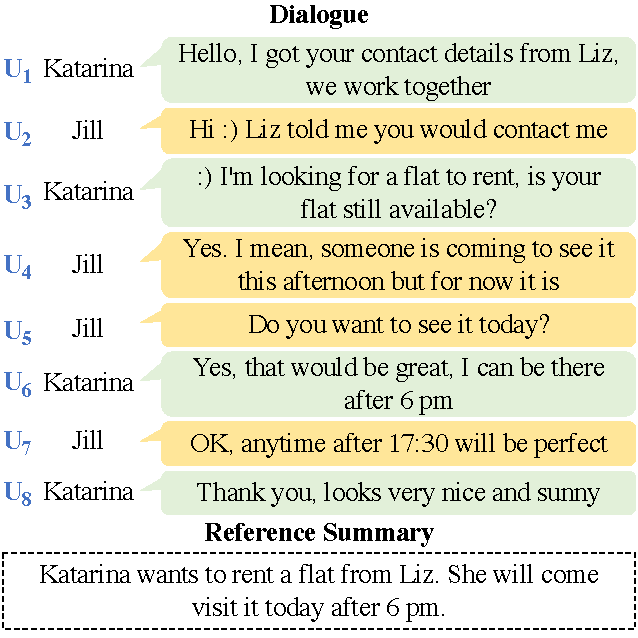
\includegraphics[scale=0.5]{fig/example.pdf}
	\caption{An example multi-party dialogue and its summary. The arrows represent unsequential dependencies between utterances. Elliptical sentences are in italic.}
	\label{fig:example}
\end{figure}

\textbf{Word Level - Language Style and Format:} 
Documents in previous well-researched summarization tasks are written from the third point of view, while dialogues consist of utterances expressed by different speakers in first person. Informal and colloquial expressions are common especially for recorded dialogues from speech, such as ``Whoa'' in $U_6$ and ``u'' representing ``you'' in $U_7$ from Figure~\ref{fig:example}.
Pronouns are frequently used to refer to events or persons mentioned in the dialogue history. Around 72\% of mentions in the conversation are {anaphoras} %pronouns
as stated in \citet{bai2021joint}. Meanwhile, the performance of coreference resolution models trained on normal text drops dramatically on dialogues~\cite{liu2021coreference}. It manifests the existence of language style differences between documents and dialogues, leading to difficulties in understanding the mappings between speakers and events in dialogues.


\textbf{Sentence/Utterance Level - Information Density:}
Document sentences are more self-contained with complete SVO (subject-verb-object) structures, while elliptical utterances are ubiquitous in dialogues, including $U_3$, $U_6$, $U_7$, $U_{11}$ and $U_{12}$.
Besides, the long dialogue can be summarized into a single summary sentence for the example in Figure~\ref{fig:example} as a result of back-and-forth questions and confirmations among speakers for communication purposes.
Question answerings, acknowledgments, and comments~\cite{asher2016discourse} are frequent discourse relations among utterances to narrow down speakers' information gaps and reach agreements.
In this way, dialogue utterances are highly content-dependent, and the information is scattered~\cite{zhang2021exploratory}, raising the difficulties for generating integral contents.

\textbf{Inter-sentence/utterance Level - Discourse structure:}
Articles tend to be well-structured, such as 
general-to-specific structure or deductive order. 
For example, the most important information 
in news summarization are always at the beginning of the document, resulting in a competitive performance of the simple Lead-$3$ baseline~\cite{nallapati2017, see2017get}. However, it is not the same for dialogue summarization. Both Lead-$3$ and Longest-$3$, i.e. $\{U1, U2, U3\}$ and $\{U4, U8, U9\}$ in Figure~\ref{fig:example}, get poor results in different dialogue scenarios~\cite{gliwa2019samsum,chen2021dialsumm,zhang2021emailsum}.
The dependencies among utterances are interleaved, shown by arrows in Figure~\ref{fig:example}, and discourse relations in dialogues are more flexible,
even with the correction of wrong information~\cite{asher2016discourse}. 
For example, 
Jake refused to be available for the reunion in $U_6$, but later agreed
in $U_8$.  As a result, it is more challenging to reason cross utterances for 
dialogue summarization than document summarization.

\textbf{Passage/Session Level - Topic boundaries:} Sentences under the same topic in documents are collected together in a paragraph or a section.
Previous works for extractive~\cite{xiao2019extractive} and abstractive summarization~\cite{cohan2018discourse} both took advantage of such features and made great progress. 
However, a dialogue is a stream of continuous 
utterances without boundaries, even for hours of discussion. The same topic may be discussed repeatedly 
with redundancies and new information, setting up obstacles for content 
selection in dialogue summarization.

%\JQ{it will be good to see the advantages of abstractive vs extractive approaches for dialogue summarization.}
%\JQ{add a little more about extractive methods, and explain why abstractive is more preferred especially in the case of dialogues.}
To better explain why abstractive approaches are more preferred than extractive ones for dialogues, we list the result of the best rule-based extractive baseline, i.e., Longest-$3$~\cite{gliwa2019samsum}, the oracle extractive result determined by Rouge-L Recall score between each summary sentence and dialogue utterances~\cite{chen2018fast}, and the generation by BART fine-tuned on SAMSum dataset~\cite{gliwa2019samsum} of the simple dialogue in Figure~\ref{fig:example} as follows:
\\
\begin{tabular}{|p{1.5cm}|p{\linewidth-2.3cm}|}
	\hline
	\textbf{Longest-$3$} & Jessica: If I move some things around, I can too! Jake: Hell yeah man! You know I freelance, worst case scenario I'll work from wherever we are Jessica: We should meet up where we did last time, it's perfect middle for everyone.\\
	\hline
	\textbf{Oracle} & Jake: Hell yeah man! You know I freelance, worst case scenario I'll work from wherever we are\\
	\hline
	\textbf{BART}& Ted, Pia, Jessica and Jake are going to meet up on Friday night. \\
	\hline
\end{tabular}
\\
We can see that the readability of generated summaries are poor for Longest-$3$ and Oracle due to the language style and format difference. The compression ratio of Longest-$3$ is apparently low while it still misses the involvement of Ted and Pia as a result of low information density of dialogues. Oracle is concise but much more information is missing. Meanwhile, the fine-tuned BART as an abstractive approach shows the favorable performance. Therefore, abstractive approaches becomes the mainstream in researches on dialogue summarization. In a word, dialogue summarization is an valuable research direction in summarization, where the modeling and understanding of dialogues are challenging compared with document summarization and abstractive approaches are especially preferred.
% despite some extractive summarization works~\cite{uma2022comparing,kano2020identifying,bokaei2016extractive}.
%@article{uma2022comparing,
%	title={Comparing Methods for Extractive Summarization of Call Centre Dialogue},
%	author={Uma, Alexandra N and Sityaev, Dmitry},
%	journal={arXiv preprint arXiv:2209.02472},
%	year={2022}
%}

%@inproceedings{kano2020identifying,
%	title={Identifying implicit quotes for unsupervised extractive summarization of conversations},
%	author={Kano, Ryuji and Miura, Yasuhide and Taniguchi, Tomoki and Ohkuma, Tomoko},
%	booktitle={Proceedings of the 1st Conference of the Asia-Pacific Chapter of the Association for Computational Linguistics and the 10th International Joint Conference on Natural Language Processing},
%	pages={291--302},
%	year={2020}
%}

%@article{bokaei2016extractive,
%	title={Extractive summarization of multi-party meetings through discourse segmentation},
%	author={Bokaei, Mohammad Hadi and Sameti, Hossein and Liu, Yang},
%	journal={Natural Language Engineering},
%	volume={22},
%	number={1},
%	pages={41--72},
%	year={2016},
%	publisher={Cambridge University Press}
%}


\subsection{Scenarios for Dialogue Summarization}\label{sec:scenarios}

Considering the source of dialogues and the purpose of doing summarization,
%\KZ{Rephrase this: dialogue sources and summary intentions}, 
we divide the application scenarios into two classes: \textbf{open-domain dialogue summarization (ODS)} and \textbf{task-oriented dialogue summarization (TDS)}. This taxonomy is similar to the one of dialogue systems~\cite{gao2020standard,chen2017survey}.
However, one should note that a pre-defined domain ontology for dialogues is 
not necessarily required for TDS, which is different from that in 
task-oriented dialogue systems.
The application scenarios investigated in previous papers 
are classified into these two classes as shown in Figure~\ref{fig:scenario}.

%\JQ{add citations}
Open-domain dialogue summarization is further divided into daily chat, 
drama conversation, debate \& comment. 
\textbf{Daily chat}~\cite{gliwa2019samsum,chen2021dialsumm} refers to the dialogues happening in our daily lives, 
such as making appointments, discussions between friends, etc. 
\textbf{Drama conversation}~\cite{rameshkumar2020storytelling,zhu2021mediasum,malykh2020sumtitles,chen2021summscreen} represents dialogues from soap operas, 
movies or TV shows, which are dramatized or fabricated with drama scripts 
behind them. Dialogues in these two classes are full of person names 
and events, resulting in narrative summaries about ``who did what''.
\textbf{Debate \& comment}~\cite{misra2015using,fabbri2021convosumm,chowdhury2019cqasumm} focuses more on question answering and 
discussions in online forums and arguments. These dialogues emphasize opinions or solutions to the given subject or questions.

Task-oriented dialogue summarization arises from application scenarios of different domains, which includes but is not limited to customer service, 
law, medical care and official issue.
\textbf{Customer service}~\cite{zou2021topic,feigenblat-etal-2021-tweetsumm-dialog,zhao2021todsum,liu2019automatic,chen2020jddc} refers to conversations between customers and service providers.
Customers start the conversation with their specific intents and agents are required to meet these requirements with the help of their in-domain databases, such as hotel reservations and express information consultation for online shopping. Dialogue summarization for this task is mainly to help service providers quickly go through solutions to users' questions for agent training and service evaluation. 
\textbf{Law}~\cite{fuzw20,duan2019legal,xi2020global} is dialogues related to legal service and 
criminal investigations. Dialogue summarization in this scenario alleviates the recording and summarizing workload 
for law enforcement or legal professionals. 
\textbf{Medical care}~\cite{joshi2020dr,song2020summarizing,song2020summarizing,zhang2021leveraging,liu2019topic} is dialogues between doctors and patients and medical dialogue summarization has some similarity to the research on electronic health records (EHR). Unlike the previous work focusing on mining useful information from EHR~\cite{yadav2018mining}, summarization is to extract useful information from the doctor-patient dialogue and generate an EHR-like or fluent summary for clinical decision-making or online search. It also aims to reduce the burden of domain experts.
\textbf{Official affair}~\cite{carletta2005ami,janin2003icsi,ulrich2008publicly,zhang2021emailsum} is conversations between colleagues for technical or teachers and students for academic issue discussion. They can be either in the format of meetings or e-mails, with summaries covering problems, solutions, and plans.


\begin{figure}
	\centering
	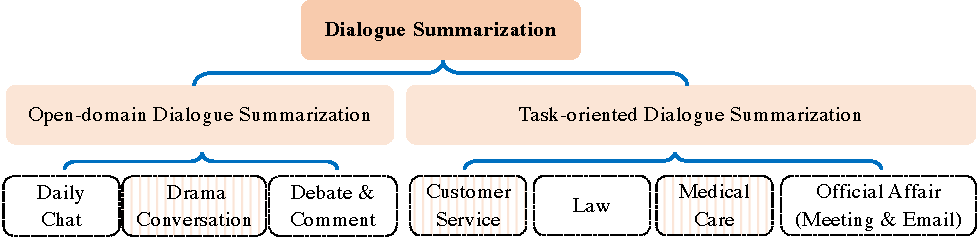
\includegraphics[scale=0.8]{fig/scenarios.pdf}
	\caption{The classification of dialogue summarization tasks with different application scenarios. Datasets proposed for evaluations under each scenario are in Section~\ref{sec:dataset}.}
	\label{fig:scenario}
\end{figure}


We compare and contrast ODS and TDS as follows.
\begin{itemize}
% functional role playing
\item Dialogues happen between \textbf{two or more speakers} both in ODS and TDS, whereas the \textbf{interpersonal relationship} and \textbf{functional relationship} among speakers are different. Generally, speakers in ODS are friends, neighbors, lovers, family members, and so on. 
They are equal either in the aspect of interpersonal relationships or functional relationships. For example, one can raise a question or answer others' questions in online forums~\cite{fabbri2021convosumm}.
In TDS, speakers have different official roles acting for corresponding responsibilities. For example, plaintiff, defendant, witness and judge in court debates~\cite{duan2019legal}, project manager, marketing expert, user interface designer and industrial designer in official meetings~\cite{carletta2005ami} are corresponding roles.
Among different dialogues, roles are the same and can be played by different speakers and a speaker's role is always unchanged for a service platform.
In a word, TDS pays more attention to functional roles while ODS focuses on speakers.


% covering topics
\item Multiple \textbf{topics} may be covered in the same dialogue session.
Topics in ODS are more diverse than in TDS. The summarization models are expected to deal with unlimited open-domain topics such as chitchat, sales, education, and climate at the same time~\cite{chen2021dialsumm}. 
However, topics in TDS are more concentrated and need more expertise for understanding.
Dialogues in TDS either focus on a single domain with more fine-grained topics, such as medical dialogues of different specialties,
or several pre-defined domains, such as restaurant, hotel, and transformation reservation.
Domain knowledge is significant for summarization, and it is divergent across sub-domains. For instance, expertise and medical knowledge are required in doctor-patient dialogues for generating accurate medical concepts~\cite{joshi2020dr} while specific knowledge bases for internal medicine and primary care are not the same.

%  inherent structure
\item The input dialogue for both ODS and TDS is made up of \textbf{a stream of utterance} as defined in Equation~\ref{eq:dialogue}. However, 
the \textbf{structure} of these two types of dialogues are different.
Open-domain dialogues often happen casually and freely while dialogues in TDS may have some inherent working procedures or writing formats. 
For example, the program manager in meetings usually masters the meeting progress~\cite{zhu2020end} implicitly with words such as ``okay, what about ...'', and communications by e-mails consist of semi-structured format including subjects, receivers, senders, and contents~\cite{zhang2021emailsum}. 

% special intentions for summaries
\item \textbf{Focuses of summaries} are distinct. Summaries for ODS in recent research are more like condensed narrative paraphrasing with different levels of granularity. An example is a synopsis from the Fandom wiki\footnote{\url{criticalrole.fandom.com}} maintained by fans for the Critical Role transcripts~\footnote{\url{github.com/RevanthRameshkumar/CRD3}}\cite{rameshkumar2020storytelling}, helping to quickly catch up with what is going on in the long and verbose dialogues. Differently, dialogues in TDS take place with strong intentions for solving problems. Summaries for such dialogues are expected to cover the user intents and corresponding solutions, such as medical summaries for clinical decision making~\cite{joshi2020dr} and customer service summaries for ticket booking~\cite{zhao2021todsum}. As a result, generating faithful content is extremely significant for TDS. %{faithfulness}
\end{itemize}

%\KZ{I feel that just dividing the dialogue summarization into ODS and TDS is a bit
%too coarse-grained. Later when you discuss the approaches, u need to associate
%each approaches with a certain characteristic/scenario of the task. It's more
%useful if u can use some refined characteristics of the task.}


\section{Evaluations}
\label{sec:evaluation}

In this section, we present a comprehensive description of existing dialogue summarization datasets 
under different scenarios and introduce several widely-accepted evaluation 
metrics for this task.
%The benchmark and some of these dataset have been concluded in \cite{feng2021survey}. So, we mainly organize features above that have been proven to be helpful for different scenarios.

\subsection{Datasets}
\label{sec:dataset}

A great number of dialogue summarization datasets have been proposed from different resources. We categorize them according to the scenarios in Section \ref{sec:scenarios}. %as shown in Figure~\ref{fig:scenario}.


\subsubsection{Open-domain Dialogue Summarization}

Open-domain dialogue summarization datasets under daily chat, drama conversation and debate\&comment are as follows and summarized in Table~\ref{tab:open}.

\textit{Daily Chat Datasets}: \textbf{SAMSum}~\cite{gliwa2019samsum} and \textbf{DialogSum}~\cite{chen2021dialsumm} are two large-scale real-life labeled datasets. Each dialogue in SAMSum is written by one person to simulate a real-life 
messenger conversations and the single reference summary is annotated by 
language experts. DialogSum, on the other hand, contains dialogues from 
the existing dialogue dataset, including DailyDialog~\cite{li2017dailydialog}, 
DREAM~\cite{sun2019dream} and MuTual~\cite{cui2020mutual}, and other English-speaking practice websites. These spoken dialogues have a more formal style than those in SAMSum, and each is accompanied by three reference summaries in the test set.  %\citet{chen2021dialsumm} claims that DialSumm is a more challenging dataset with a lower compression ratio and more diverse topics than SAMSum. 
Besides, AIHub Dialogue Summarization Dataset (\textbf{HubDial})~\footnote{https://aihub.or.kr/} also contains dialogues covering a range of daily topics.

 
%Dramatic dialogues represent the dialogues on TV which are likely to have drama scripts behind them.
\textit{Drama Conversation Datasets}: \textbf{CRD3}~\cite{rameshkumar2020storytelling} is collected from a live-stream role-playing game called Dungeons and Dragons, which is more amenable to extractive approaches with low abstractiveness.
%The dataset consists of 159-episode dialogue transcripts and summaries with extremely long texts, and they further segment paired texts into dialogue-summary chunks with reasonable lengths for training with neural networks. 
%CRD3 is more amenable to extractive approaches with low abstractiveness.
 \textbf{MediaSum}~\cite{zhu2021mediasum} includes interview transcripts from 
NPR and CNN and their reviews or topic descriptions are regarded as the 
corresponding summaries. The large size of this automatically crawled 
dataset makes it particularly suitable for pre-training. %for zero-shot or few-shot applications.
Other two datasets are collected from a variety of movies and TV series, 
including \textbf{SubTitles}~\cite{malykh2020sumtitles} and 
\textbf{SummScreen}~\cite{chen2021summscreen}. Dialogues are corresponding 
transcripts, and summaries are aligned synopses or recaps 
written by humans.
%According to dataset styles and dialogue-summary aligning approaches, \textbf{SubTitles}~\cite{malykh2020sumtitles} consists of Subtitiles, Scripts and Gold, and \textbf{SummScreen}~\cite{chen2021summscreen} consists of TMS and FD. 
%The alignment in Scripts are done automatically with multiple similarity functions, while Gold are done by human annotators.
%Summaries form Subtitles are high-level plot summaries describing a movie or a series episode in no more than ** words compared with Scripts and Gold.
%TMS focus more on dialogues with more details in the corresponding summaries, while FD have more descriptions about environments or character actions with shorter summaries.
 
%Dialogues rich in discussions and comments are also a representative application scenario. For example, people may discuss about politics or world affairs online after they go through the corresponding news.
%Summarizing such dialogues helps people know better about the world.
 \textit{Debate\&Comment Datasets}: \textbf{ADSC}~\cite{misra2015using} 
is a test-only dataset extracted from the Internet Argument 
Corpus~\cite{walker2012your}. It contains 45 two-party dialogues about gay 
marriages, each  associated with 5 reference summaries. 
\textbf{FORUM}~\cite{tarnpradab2017toward} contains human-annotated forum threads collected from tripadvisor.com and ubuntuforums.org.
Three out of four sub-datasets in \textbf{ConvoSumm}~\cite{fabbri2021convosumm} 
are similar discussions, including news article comments (\textbf{NYT}), 
discussion forums and debate (\textbf{Reddit}) and community question answers 
(\textbf{Stack}) from different sources. Each sample has a human-written reference.
\textbf{CQASUMM}~\cite{chowdhury2019cqasumm} is another community question 
answering dataset but without back and forward discussions among speakers. The summary here aims to summarize multiple answers, which is closer to a multi-document summarization setting.
% which is more similar to \KZ{rephrase: a multi-document summarization setting among answers without discussions between multiple interlocutors.}%The labeled summaries are relative small with 250 development and 250 test examples respectively.

\begin{table}[th]
	\centering
	\small
		\begin{tabular}{|l|c|c|c|c|c|p{4cm}|c|}
			%|l|c|c|c|c|c|c|
			\hline
			\textbf{\makecell[c]{Name}} & \textbf{\makecell{$\#$Samples \\ train/val/test}} & \textbf{$\#$Spk} & \textbf{Lang.} & \textbf{DW} & \textbf{SW} & \textbf{\makecell[c]{Download Link}} & \textbf{AVL} \\
			\hline
			\multicolumn{6}{|l|}{\bf \em{Daily Chat}} \\
			\hline
			%\tabincell{c}{SAMSum\cite{gliwa2019samsum}} & 14,732/818/819 & $\geq$2 & Eng. & \tabincell{l}{https://www.tensorflow.org/\\datasets/catalog/samsum}& Y \\
			%\hline
			SAMSum\cite{gliwa2019samsum} & 14.7k/0.8k/0.8k%14,732/818/819 
			& $\geq$2 & English & 94 & 25 & \tabincell{l}{https://huggingface.co/datasets\\/samsum}& Y \\
			\hline
			DialogSum\cite{chen2021dialsumm} & 12.5k/0.5k/0.5k%12,460/500/500 
			& 2& English & 131 & 22 &\tabincell{l}{https://github.com/cylnlp/\\DialogSum} & Y\\
			
			\hline
			HubDial & 350k & $\geq$2 & Korean & - & - &\tabincell{l}{https://aihub.or.kr/}  & C \\
			
			\hline
			%GupShup\cite{mehnaz2021gupshup} & 5.8k/0.5k/0.5k %5,831/500/500
			%& $\geq$2 &  \tabincell{l}{Hindi-\\English} & ** & ** & \tabincell{l}{https://huggingface.co/\\midas/gupshup\_h2e\_mbart} &Y \\
			%\hline
			\multicolumn{6}{|l|}{\bf \em{Drama Conversation}} \\
			\hline
			CRD3\cite{rameshkumar2020storytelling} &	26.2k/3.5k/4.5k %26,232/3,470/4,541 
			& $\geq$2 & English & 31,803 & 2,062 & \tabincell{l}{https://github.com/\\RevanthRameshkumar/CRD3}& Y \\
			\hline
			MediaSum\cite{zhu2021mediasum} &
			463.6k/10k/10k %463,6000/10,000/10,000
			& $\geq$2 & English & 1,554 & 14 & \tabincell{l}{https://github.com/\\zcgzcgzcg1/MediaSum/}& Y \\
			\hline
			\makecell[l]{SumTitles\cite{malykh2020sumtitles}\\(Subtitiles/Scripts/Gold)} & \makecell[c]{132k\\21k\\290}%153k 
			& $\geq$2 & English & \makecell[c]{6,406\\423\\395} & \makecell[c]{85\\55\\51} & \tabincell{l}{https://github.com/huawei-\\noah/noah-research/tree/\\master/SumTitles}& Y \\
			\hline
			\makecell[l]{SummScreen\cite{chen2021summscreen}\\(FD/TMS)} &\makecell[c]{3,673/338/337\\18,915/1,795/1,793} %22.6k/2.1k/2.1k %22,588/2,133/2,130
			& $\geq$2 & English & \makecell[c]{7,605\\6,421} & \makecell[c]{114\\381} & \tabincell{l}{https://github.com/mingdachen\\/SummScreen}& Y \\
			\hline
			\multicolumn{6}{|l|}{\bf \em{Debate \& Comment}} \\
			\hline
			ADSC\cite{misra2015using} & 45 & 2 & English & 672 & 151 &\tabincell{l}{https://nlds.soe.ucsc.edu/\\summarycorpus}& Y \\
			\hline
			CQASUMM\cite{chowdhury2019cqasumm} & 100k
			& $\geq$2 & English& 782 & 100 &\tabincell{l}{https://bitbucket.org/tanya1410\\9/cqasumm/src/master/} & Y\\
			
			\hline
			FORUM~\cite{tarnpradab2017toward} & 689 & $\geq$2 & English & 825 & 191 &  \tabincell{l}{http://tinyurl.com/jcqgcu8} & Y \\
			
			\hline
			\makecell[l]{ConvoSumm\cite{fabbri2021convosumm}\\(NYT/Reddit/Stack)} &  \makecell[c]{-/0.25k/0.25k\\-/0.25k/0.25k\\-/0.25k/0.25k}
			& $\geq$2 &  \tabincell{l}{English}& \makecell[c]{1,624\\641\\1,207} & \makecell[c]{79\\65\\73} & \tabincell{l}{https://github.com/\\Yale-LILY/ConvoSumm} &Y \\
			
			\hline
			
		\end{tabular}
		\caption{Open-domain dialogue summarization datasets. ``Lang.''  and ``Spk'' stands for ``Language'' and ``Speakers''. ``DW'' and ``SW'' represents the average number of words in the dialogues and summaries respectively. ``AVL'' refers to the public availability of the
dataset ($Y$ is available, $N$ is not available, and $C$ is conditional). HubDial is only available for Koreans.}%\JQ{the average source content length (word and utterance) and summary length in Table 1 and Table 2}}
%\KZ{Change D to C (conditional)?}}	
		\label{tab:open}		
\end{table}


\subsubsection{Task-oriented Dialogue Summarization}

Datasets here are rooted in specific domains, including
customer service, law, medical care and official issue. We list them in Table~\ref{tab:task}. 

%With the rapid development of Internet services, online customer service becomes important increasingly. 
%In the e-commerce scenario,
\textit{Customer Service Datasets}: Zou et al.\shortcite{zou2021topic,zou2021unsupervised} propose two similar datasets with summaries from the agent perspective.
\citet{lin2021csds} provides a more fine-grained dataset \textbf{CSDS} containing a user summary, an agent summary, and an overall summary based on JDDC dataset~\cite{chen2020jddc}. %\citet{zou2021unsupervised} also mentioned a similar dataset.
Summaries from \textbf{Didi dataset}~\cite{liu2019automatic} are also written from agents' points of view, in which dialogues are about transportation issues instead of pre-sale and after-sale topics in the former one.
More complicated multi-domain scenarios are covered in \textbf{TWEETSUMM}~\cite{feigenblat-etal-2021-tweetsumm-dialog}, \textbf{MultiWOZ*}~\cite{yuan2019scaffolds} and \textbf{TODSum}~\cite{zhao2021todsum}. Dialogues from TWEETSUMM spread over a wide range of domains, including gaming, airlines, retail, and so on. 
MultiWOZ* and TODSum transform and annotate summaries based on the original MultiWOZ dataset~\cite{eric2019multiwoz}.
There are also two earlier datasets called \textbf{DECODA} and \textbf{LUNA}~\cite{favre2015call} containing call centre conversations with synopses summarizing the problem of the caller and how it is solved.  
%\KZ{What does this mean: contains domain transitions and inherent domain ontology within a dialogue}.
%Dialogues in this dataset are collected based on (domain, intent, slot, value) tuples according to a structured ontology based on domain knowledge.




\begin{table}[t]
	\centering
	\small		
		\begin{tabular}{|l|c|c|c|c|c|p{3.7cm}|c|}
			\hline
			\textbf{\makecell[c]{Name}} &\textbf{ \makecell{$\#$Samples \\ train/val/test}}& \textbf{$\#$Spk} & \textbf{Lang.} & \textbf{DW} & \textbf{SW} & \textbf{\makecell[c]{Download Link}} & \textbf{AVL} \\
			\hline
			\multicolumn{6}{|l|}{\bf \em{Customer Service}} \\
			
			\hline
			\citet{zou2021topic} & 17.0k/0.9k/0.9k%18.86k 90%/5%/5% 
			& 2 & Chinese & 1,334 & 55 &\tabincell{l}{https://github.com/RowitZou\\/topic-dialog-summ}& Y \\
			
			\hline
			CSDS\cite{lin2021csds} & 9.1k/0.8k/0.8k%9,101 / 800 / 800
			& 2& Chinese & 401 & 83 &\tabincell{l}{https://github.com/xiaolin\\Andy/CSDS} & Y\\
			
			\hline
			{\citet{zou2021unsupervised}} & -/0.5k/0.5k%1.09M chat logs
			& 2 &  \tabincell{l}{Chinese}& 95 & 37 & \tabincell{l}{https://github.com/RowitZou\\/RankAE} &Y \\
			
			\hline
			{Didi\cite{liu2019automatic}} &296.3k/2.9k/29.6k %26,232/3,470/4,541 
			& 2 & Chinese & - & - &	\tabincell{l}{-}& N \\
			
			\hline
			{TWEETSUMM\cite{feigenblat-etal-2021-tweetsumm-dialog}} & 0.9k/0.1k/0.1k %1.1k 80%/10%/10%
			& 2 & English & 245 & 36 & \tabincell{l}{https://github.com/guyfe\\/Tweetsumm}& Y \\
			
			
			\hline
			MultiWOZ*\cite{yuan2019scaffolds} & 8.3k/1k/1k & 2 & English & 181 & 92 & \tabincell{l}{https://github.com/voidforall\\/DialSummar}& Y\\
			
			\hline
			{TODSum\cite{zhao2021todsum}} & 9.9k & 2 & English & 187 & 45 &\tabincell{l}{-}& N \\
			
			\hline
			DECODA\cite{favre2015call} & -/50/100 & 2 & \makecell[c]{French/\\English}
			& \makecell[c]{42,130\\41,639} & \makecell[c]{23\\27} & \tabincell{l}{https://pageperso.lis-lab.fr/\~benoit\\.favre/cccs/} & C\\
			
			\hline
			LUNA\cite{favre2015call} & -/-/100 & 2 & \makecell[c]{Italian/\\English}
			& \makecell[c]{34,913\\32,502} & \makecell[c]{17\\15}  &\tabincell{l}{https://pageperso.lis-lab.fr/\~benoit\\.favre/cccs/}  & C\\
			
			\hline
			\multicolumn{6}{|l|}{\bf \em{Law}} \\
			
			\hline
			{Justice\cite{fuzw20}} & 30k%14,732/818/819 
			& 2 & Chinese & 605 & 160 & \tabincell{l}{-}& N \\
			
			\hline
			{PLD\cite{duan2019legal}} & 5.5k& $\geq$2 & English  & - & - &\tabincell{l}{https://github.com/zhouxinhit\\/Legal\_Dialogue \_Summarization} & C \\
			
			\hline
			{LCSPIRT-DM\cite{xi2020global}} &  30.8/3.8k/3.8k%38.5k 80%/10%/10%
			& 2 &  Chinese& 684 & 75 & \tabincell{l}{http://eie.usts.edu.cn/prj/\\NLPoSUST/LcsPIRT.htm} & C \\
		
			\hline
			\multicolumn{6}{|l|}{\bf \em{Medical Care}} \\
		
			\hline
			{\citet{joshi2020dr}} & 1.4k/0.16k/0.17k%1365 /158/167 
			& 2 & English & - & - &\tabincell{l}{-}& N \\
			
			\hline
			{\citet{song2020summarizing}} & 36k/-/9k %35987/8996
			& 2& Chinese  & 312 & 23/113 &\tabincell{l}{https://github.com/cuhksz-nlp\\/HET-MC} & Y\\
			
			\hline
			{\citet{liu2019topic}} & 100k/1k/0.49k
			& 2 &  \tabincell{l}{English}& - & - & \tabincell{l}{-} &N \\
			
			\hline
			{\citet{zhang2021leveraging}} & 0.9k/0.2k/0.2k %939(15043), 201(3095), and 202(3450),
			& 2 & English & - & - & \tabincell{l}{-}& N \\
			
			\hline
			\multicolumn{6}{|l|}{\bf \em{Official Issue (Meeting \& Emails)}} \\
			
			\hline
			{AMI\cite{carletta2005ami}} &137 %142 
			& $>$2 & English & 4,757 & 322 & \tabincell{l}{https://groups.inf.ed.ac.uk/ami}& Y \\
			
			\hline
			{ICSI\cite{janin2003icsi}} & 59 %75 
			& $>$2 & English & 10,189 & 534 &\tabincell{l}{https://groups.inf.ed.ac.uk/ami\\/icsi}& Y \\
			
			\hline
			{QMSum\cite{zhong2021qmsum}} & 1.3k/2.7k/2.7k% 1,257 / 272 / 279 
			& $>$2 & English & 9070 & 70 &\tabincell{l}{https://github.com/Yale-LILY\\/QMSum}& Y \\
			
				\hline
			{Kyutech\cite{yamamura2016kyutech,nakayama2021corpus}} &  9 
			& $>$2 & Japanese & - & - &\tabincell{l}{http://www.pluto.ai.kyutech.\\ac.jp/~shimada/resources.html}& Y \\
			
			\hline
			{BC3\cite{ulrich2008publicly}} & 30%1800/249/500
			& $>$2 & English & 550 & 134 &\tabincell{l}{https://www.cs.ubc.ca/cs-\\research/lci/research-groups\\/natural-language-processing\\/bc3.html} & Y \\
			
			\hline
			{\citet{loza2014email}} & 107%1800/249/500
			& $>$2 & English & - & - &\tabincell{l}{-} & N\\
			
			\hline
			{EmailSum\cite{zhang2021emailsum}} & 1.8k/0.25k/0.5k%1800/249/500
			& $\geq$2 & English& 233 & 27/69 &\tabincell{l}{https://github.com/ZhangShiyue\\/EmailSum} & C \\
			
			\hline
			\makecell[l]{ConvoSumm\cite{fabbri2021convosumm}\\(Email)} &  -/0.25k/0.25k%
			& $\geq$2 &  \tabincell{l}{English} &917 & 74 & \tabincell{l}{https://github.com/Yale-LILY\\/ConvoSumm} &Y \\
			
			\hline
		
		\end{tabular}	
		\caption{Task-oriented dialogue summarization datasets. The original text data is not accessible for PLD due to privacy issues. DECODA, LUNA and LCSPIRT-DM can only be obtained through an application. EmailSum is not free.}
		\label{tab:task}
	%\caption{Dialogue Summarization Datasets}	
\end{table}


%Courts and police are meaningful scenarios for releasing the rising workload.
\textit{Law Datasets}: \textbf{Justice}~\cite{fuzw20} includes 
debates between a plaintiff and a defendant on some controversies 
which take place in the courtroom. The final factual statement by the 
judge is regarded as the summary.
A similar scenario is included in \textbf{PLD}~\cite{duan2019legal}, which is more 
difficult to summarize due to the unknown number of participants. There is also another version 
of PLD by~\citet{gan2021inspectional} with fewer labeled cases than the 
original PLD.
\citet{xi2020global} proposed a long text summarization dataset \textbf{LCSPIRT-DM} based 
on police inquiry records full of questions and answers.


\textit{Medical Care Datasets}:
%Medical care are heath consultation dialogues between doctors and patients. 
Both \citet{joshi2020dr} and \citet{song2020summarizing} proposed medical summarization corpora by crawling data from online health platforms and annotating coherent summaries by doctors. \citet{song2020summarizing} also proposed one-sentence summaries of medical problems uttered by patients, whereas \citet{liu2019topic} used simulated data with summary notes in a very structured format.
 \citet{zhang2021leveraging} used unreleased dialogues with coherent summaries of the history of the present illness. %which is less structured.

%Official affairs are familiar in work. Most of them are face-to-face real-time meetings, resulting in verbose transcripts. Summarizing keynotes among the meeting can enhance the efficiency of work. 
\textit{Official Issue Datasets}: \textbf{AMI}~\cite{carletta2005ami} and \textbf{ICSI}~\cite{janin2003icsi} are meeting transcripts concerning 
computer science-related issues in working background and research background, respectively. Both datasets are rich in human labels, including extractive summary, abstractive summary, topic segmentation, and so on. They are also included in \textbf{QMSum}~\cite{zhong2021qmsum} and are further labeled for query-based meeting summarization. \textbf{Kyutech}~\cite{yamamura2016kyutech} is a similar dataset in Japanese containing multi-party conversations, where the participants pretend to be managers of a virtual shopping mall in a virtual city and do some decision-making tasks. Their later work~\cite{nakayama2021corpus} annotated more fine-grained summaries for each topic instead of the whole conversation in ~\cite{yamamura2016kyutech}.
In addition, official communications are also prevalent in e-mails. 
\citet{ulrich2008publicly} propose the first email summarization dataset \textbf{BC3} with only 30 threads and \citet{loza2014email} release 107 email threads. Both of them contain extractive as well as abstractive summaries.
EmailSum~\cite{zhang2021emailsum} has both a human-written short summary and a long summary for each e-mail thread. 
Besides, Email threads (\textbf{Email}) in ConvoSumm~\cite{fabbri2021convosumm} have only one abstractive summary for each dialogue.


\subsubsection{Summary}
We make the following observations and conclusions.
\begin{itemize}
	\item The size of dialogue summarization datasets is much smaller than document summarization datasets. Most dialogue summarization datasets have no more than $30K$ samples, while representative document summarization datasets, such as CNNDM and XSum, have more than $200K$ samples. Datasets for drama conversations are relatively larger and can be potential pre-training data for other scenarios.
%	\KZ{Try to avoid passive voice: which are potentially to be used} as pre-training data for other scenarios.
	\item The number of interlocutors in different dialogue summarization scenarios is different. Most ODS dialogues have more than $2$ speakers while 
most dialogues in TDS have only 2 speakers except in official meetings or 
e-mails.
	\item TDS dialogues tend to be more private. Thus, half of the 
TDS datasets are not publicly available, especially for Law and 
Medical Care scenarios. 
	\item Datasets with more than 2,048 dialogue words, which is the upper bound of the input length of most pre-trained language models, are suitable for research on long dialogue summarization. They contain both open-domain datasets and task-oriented datasets. 
	 %including CRD3~\cite{rameshkumar2020storytelling}, MediaSumm~\cite{zhu2021mediasum}, SumTitles~\cite{malykh2020sumtitles}, SummScreen~\cite{chen2021summscreen} and ConvoSumm~\cite{fabbri2021convosumm}, and task-oriented datasets including AMI~\cite{carletta2005ami}, ICSI~\cite{janin2003icsi}, QMSum~\cite{zhong2021qmsum} and~\citet{zou2021topic}'s customer service dataset.
	%It points out a need of a taxonomy on different techniques instead of listing approaches under different datasets, which should be more effective when facing a new scenarios with some collected data. 
\end{itemize} 
 


%\subsection{Privacy Concerns}
%Due to privacy and ethical issues of dialogues, 
%different focus on different extract or abstract, faithfulness

\subsection{Evaluation Metrics}
\label{sec:evalmetric}
In existing works, \textit{Automatic evaluation metrics} commonly used for summarization such as \textbf{Rouge}~\cite{lin2004rouge}, \textbf{MoverScore}~\cite{zhao2019moverscore}, \textbf{BERTScore}~\cite{zhang2019bertscore} and \textbf{BARTScore}~\cite{yuan2021bartscore} are also used for dialogue summarization by comparing the generations with references. However, these widely-accepted metrics' performance may deviate from human~\cite{chen2021dialsumm,hanna2021fine}, especially in the aspect of consistency. Therefore, more focussed evaluation metrics and human evaluations emphasizing \textit{information coverage} and \textit{factual consistency} are considered as follows.
%\KZ{To complement these metrics qualifying the overall matching degree to the 
%reference}, 

Instead of comparing only with the whole reference summary, most researches for TDS only consider key words/phrases
while ignoring other common words for measuring the \textbf{information coverage}.  In other words, evaluation for TDS emphasizes the coverage of key information which are generally domain-specific terms and can be easily recognized.
%moves towards accurate summaries 
For example, {medical concept coverage}~\cite{joshi2020dr,zhang2021leveraging} 
and {critical information completeness}~\cite{yuan2019scaffolds} both
extract essential phrases based on domain dictionaries by 
rules or publicly available tools. 
\citet{zhao2021give} uses slot-filling model~\cite{chen2019bert} to recognize slot values for {factual completeness}.
Then, the accuracy or F1 scores are 
calculated by comparing extracted phrases or concepts from $Y$ and $Y'$. 



%Besides these extraction-based metrics, reference-free evaluation metrics~\cite{shao2017efficient,durmus2020feqa,egan2022play,liu2022reference} are gaining more and more attention. 
%Some of them have been adopted for dialogue summarization for measuring \textbf{the factual consistency} of generations given source dialgoue.

ODS pays less attention to information coverage due to the higher subjectivity on salient information selection. Instead, measuring the \textbf{factual consistency} of generations gains increasing attention. Unlike the above metrics which compare generations with the reference summary, 
most evaluation metrics here compare generations with the source dialogue and can be classified into reference-free evaluation metrics~\cite{shao2017efficient,durmus2020feqa,egan2022play,liu2022reference}.
A QA-based model~\cite{wang2020asking} is borrowed by \citet{zhao2021give}.
It follows the idea that factually consistent summaries and documents generate the same answers to a question.
NLI-based methods~\cite{maynez2020faithfulness} that require the content in the summary to be fully inferred from the dialogue were adopted by~\citet{liu2022data}.
\citet{liu2021controllable} automatically evaluate {inconsistency} issues 
of person names by using noised reference summaries as negative samples and training a BERT-based binary classifier.
\citet{asi2022end} used the FactCC metric from~\citet{kryscinski2020evaluating} where the model was trained only with source documents with a series of rule-based transformations.
Information correctness of the generated summary is also important for TDS. For instance, negation correctness as a specific consistency type is considered by ~\citet{joshi2020dr} with 
publicly available tools Negex~\cite{harkema2009context} for recognizing 
negated concepts.

Meanwhile, \textit{human evaluations} are required to complement the above metrics.
Besides ranking or scoring the generated summary with an overall quality score~\cite{chen2020multi}, 
more specific aspects are usually provided to annotators. Representative ones include:
\textbf{readability/fluency}~\cite{yuan2019scaffolds,zhao2021give} requiring a summary to be grammatically correct and well structured,
\textbf{informativeness}~\cite{feng2020dialogue,lei2021finer,feigenblat-etal-2021-tweetsumm-dialog,feng2021language} measuring how well the summary includes salient information,
\textbf{conciseness/non-redundancy}~\cite{feng2021language,yuan2019scaffolds} pursuing a summary without redundancy,
and \textbf{factualness/consistency}~\cite{feng2020dialogue,zhao2021give,lei2021finer,kim2022mind} evaluating whether the summary is consistent with the source dialogue. There are also some typical fine-grained metrics evaluating errors in generated summaries mentioned in previous works~\cite{chen2020multi,chen2021dialsumm,liu2021coreference}: 
\textbf{Information missing} means that content mentioned in references are missing in generated summaries, while \textbf{information redundancy} is the opposite.
\textbf{Reference error} refers to wrong associations between a speaker and an action or a location.
\textbf{Reasoning error} is that the model incorrectly reasons the conclusion among multiple dialogue turns.
Moreover, \citet{chen2020multi} mentioned \textbf{improper gendered pronouns} referring to improper gendered pronouns. \citet{tang2021confit} also proposed \textbf{circumstantial error}, \textbf{negation error}, \textbf{object error}, \textbf{tense error} and \textbf{modality error} for more detailed scenarios. All of their error types can also be grouped into two classes, where the information missing and redundancy are for the coverage of key information, and the rest are for factual consistency.


A summary of evaluation metrics adopted in existing dialogue summarization works is in Table~\ref{tab:eval-metrics}.

\begin{table}[h]
	\centering
	\small
	\begin{tabular}{|l|l|p{6.8cm}|}
		\hline
		\textbf{Types} & \textbf{Description} & \textbf{Metrics} \\
		\hline
		\multirow{3}{*}{Automatic Evaluation} & Commonly-used & Rouge, MoverScore, BERTScore, BARTScore, ... \\
		\cline{2-3}
		 & Information Coverage & medical concept coverage, critical information completeness, factual completeness, ...\\
		 \cline{2-3}
		 & Factual Consistency & QA-based metrics, NLI-based metrics, binary classifiers with synthetic data, negation correctness, ...\\
		 \hline
		\multirow{3}{*}{Human Evaluation} & Evaluation Aspects& readability / fluency, informativeness, conciseness / non-redundancy, factualness / consistency\\
		\cline{2-3}
		& Error Types & {information missing, information redundancy, reference error, reasoning error, improper gendered pronouns, circumstantial error, negation error, object error, tense error, modality error} \\ 
		\hline
		
	\end{tabular}
	\caption{A summary of evaluation metrics.}
	\label{tab:eval-metrics}
\end{table}

%including readability/fluency~\cite{yuan2019scaffolds,zhao2021give}, completeness~\cite{lei2021finer}, informativeness~\cite{feng2020dialogue,lei2021finer,feigenblat-etal-2021-tweetsumm-dialog,feng2021language}, conciseness/non-redundancy~\cite{yuan2019scaffolds}, consistency/factualness~\cite{feng2020dialogue,zhao2021give,lei2021finer} and coherence.
%Information missing, information redundant, reference error, reasoning error, 
%improper gender pronouns and tense consistency are typical fine-grained metrics evaluating 
%errors in generated summaries.

%Some specially designed metrics are introduced for specific purpose, such as medical concept coverage~\cite{joshi2020dr,zhang2021leveraging} and negation correctness~\citet{joshi2020dr} which are important factors contributing to accurate medical summaries. These evaluating targets are extracted either utilizing domain dictionaries with rules or publicly available tools, such as quickUMLS~\footnote{\url{https://www.nlm.nih.gov/research/ umls/index.html}} for medical concepts and Negex~\cite{harkema2009context} for recognizing negated concepts. 
%\citet{zhao2021give} propose factual consistency and factual completeness based on pretrained QA-based model~\cite{wang2020asking} and slot-filling model~\cite{chen2019bert}.
%\citet{liu2021controllable} trains a BERT-based binary classifier for detecting inconsistency issues of person names between dialogues and the summaries. 

%\citet{yuan2019scaffolds} proposed Critical Information Completeness for computing the matched predefined essential entities or slots in $Y$ and $Y'$, ignoring other common words or phrases.


\section{Experiments}

\label{sec:experiment}

%\begin{table*}[th!]
%   \centering
%   \scriptsize
%   \begin{tabular}{l|llcc}
%       \toprule
%       \textbf{Dataset} &\textbf{Premise}  & \textbf{Choices} & \textbf{Training size} & \textbf{Test size}\\
%       \midrule
%       \multirow{4}{*}{ROC} & Sarah was home alone. &\multirow{2}{*}{Sarah then happily watched the show.     %\checksymbol}&\multirow{4}{*}{1871}&\multirow{4}{*}{1871}\\
%                       &She wanted to stay busy. &     \multirow{2}{*}{Sarah could not find anything to watch. \crosssymbol } \\
%                       &She turned on the TV. \\
%                       &She found a reality show to watch.\\
%       \midrule
%       \multirow{3}{*}{ARCT} &\textbf{Reason}: Milk isn’t a gateway drug even though &\textbf{Warrant 1}: Milk is similar to marijuana. \checksymbol&\multirow{3}{*}{1210}&\multirow{3}{*}{444}\\
%       &most people drink it as children. &\textbf{Warrant 2}: Milk is not marijuana.\crosssymbol \\
%       &\textbf{Claim}: Marijuana is not a gateway drug. \\
%       \midrule
%       \multirow{4}{*}{RECLOR} &\textbf{Context}:In a business...to financial prosperity. &A: ignores the fact that in... the family 's prosperity.\checksymbol&\multirow{4}{*}{4638}&\multirow{4}{*}{500}\\
%       &\textbf{Question}:The reasoning in the argument&B: presumes, without... the family's prosperity.\crosssymbol&\\
%       & is flawed because the argument&C: ignores the fact... even if they pay high wages.\crosssymbol\\
%       &&D: presumes, without providing...can succeed.\crosssymbol\\
        
        
%       \bottomrule
%   \end{tabular}
%   \label{table:dataset}
%\end{table*}

%\begin{table*}[th!]
%    \centering
%    \scriptsize
%    \begin{tabular}{l|llcc}
%        \toprule
%        \textbf{Dataset} &\textbf{Premise}  & \textbf{Choices} & \textbf{Training size} & \textbf{Test size}\\
%        \midrule
%        \makecell[c]{COPA} &  \makecell[l]{I pushed the door.} &\makecell[l]{The door opened.     \checksymbol 
%        \\The door locked. \crosssymbol }&\makecell[c]{500}&\makecell[c]{500}\\
%        \midrule
%        \makecell[c]{ROC} &  \makecell[l]{Sarah was home alone.\\She wanted to stay busy.\\She turned on the TV.\\She found a reality show to watch.} &\makecell[l]{Sarah then happily watched the show.     \checksymbol 
%        \\Sarah could not find anything to watch. \crosssymbol }&\makecell[c]{1871}&\makecell[c]{1871}\\
%        \midrule
%        \makecell[c]{ARCT} &\makecell[l]{\textbf{Reason}: Milk isn’t a gateway drug even though \\ most people drink it as children. \\\textbf{Claim}: Marijuana is not a gateway drug.}&\makecell[l]{\textbf{Warrant 1}: Milk is similar to marijuana. \checksymbol \\
%        \textbf{Warrant 2}: Milk is not marijuana.\crosssymbol}&\makecell[c]{1210}&\makecell[c]{444}\\
%        \midrule
%        \makecell[c]{RECLOR} &\makecell[l]{\textbf{Context}:In a business...to financial prosperity. \\
%        \textbf{Question}:The reasoning in the argument\\  is flawed because the argument}&\makecell[l]{A: ignores the fact that in... the family 's prosperity.\checksymbol
%        \\B: presumes, without... the family's prosperity.\crosssymbol
%        \\C: ignores the fact... even if they pay high wages.\crosssymbol
%        \\D: presumes, without providing...can succeed.\crosssymbol}&\makecell[c]{4638}&\makecell[c]{500}\\
%        
%        
%        \bottomrule
%    \end{tabular}
%    \caption{Examples for all 4 datasets considered in this paper.}
%    \label{table:dataset}
%\end{table*}

\begin{table}[th!]
    \centering
    \scriptsize
    \begin{tabular}{l|ll}
        \toprule
        \textbf{Dataset} &\textbf{Premise}  & \textbf{Choices}\\
        \midrule
        \makecell[c]{COPA} &  \makecell[l]{I pushed the door.} &\makecell[l]{The door opened.     \checksymbol 
        \\The door locked. \crosssymbol }\\
        \midrule
        \makecell[c]{ROC} &  \makecell[l]{Sarah was home alone.\\She wanted to stay busy.\\She turned on the TV.\\She found a reality show to watch.} &\makecell[l]{Sarah then happily watched the show.     \checksymbol 
        \\Sarah could not find anything to watch. \crosssymbol }\\
        \midrule
        \makecell[c]{ARCT} &\makecell[l]{\textbf{Reason}: Milk isn’t a gateway drug \\
        even though most people drink it \\as children. \\\textbf{Claim}: Marijuana is not a gateway \\drug.}&\makecell[l]{\textbf{Warrant 1}: Milk is similar to marijuana. \checksymbol \\
        \textbf{Warrant 2}: Milk is not marijuana.\crosssymbol}\\
        \midrule
        \makecell[c]{RECLOR} &\makecell[l]{\textbf{Context}:In a business...to financial \\prosperity. \\
        \textbf{Question}:The reasoning in the \\argument is flawed because the \\argument}&\makecell[l]{A: ignores the fact that in... the family 's prosperity.\checksymbol
        \\B: presumes, without... the family's prosperity.\crosssymbol
        \\C: ignores the fact... even if they pay high wages.\crosssymbol
        \\D: presumes, without providing...can succeed.\crosssymbol}\\
        
        
        \bottomrule
    \end{tabular}
    \caption{Examples for all 4 datasets considered in this paper.}
    \label{table:dataset}
\end{table}



%1. Re-evaluate the extent to which the model is exploiting short circuit after augmentation. Test it on the same sampled examples to see the improvement of the percentage of cases where model look at context.

We evaluate the effectiveness of the proposed augmentation methods on four popular 
natural language reasoning tasks.
Three transformer-based models are employed as the
main targets for our experiments. 
We first show the experimental setup. 
%Second, we compare several operators for testing short circuit problem and apply the best one to multiple models on diverse NL reasoning tasks.
Then, we compare different augmentation methods on three models by the 
end-to-end tests, which contain
the stress test and original test of the four datasets, and demonstrate
the advantage of crossover and mutation. 
After that, we apply choice-only tests on the same set of models compared in the
last step, to reconfirm that performance gain in the end-to-end tests is
due to the reduction of short-circuit problems.
%Third, we reconfirm the findings in the end-to-end evaluations
%through additional choice-only tests. 
%without data augmentation 
%and of different modelswith choice-only test and 
Finally, we use a case study to discover the reason for the model improvement 
by the white-box test. 
%Finally we give a discussion about mutation augmentation method.

\subsection{Experimental Setup} 
\label{sec:setup}
% In this section, we will show our setup for datasets, models and test operators.
\subsubsection{Datasets}
We experiment on 4 datasets from four different tasks:
%\KZ{I think you need to say what is the context and what are the
%choices for these four datasets.}

\textbf{ROC} is a story ending prediction dataset. 
The task is to identify the correct ending of a four-sentence 
story premise from two alternative choices. 

\textbf{COPA} is a causal reasoning dataset, an example is previously shown
in~\secref{sec:intro}. Given a premise, 
COPA requires choosing the more plausible, causally related choice. 
%There are 500 instances in 
%training data and 500 instances for testing.

\textbf{ARCT} is an argument reasoning comprehension dataset. 
There may exist an alternative warrant choice 
in which the reason is connected to the claim.

\textbf{RECLOR} is a reading comprehension dataset that requires logical reasoning.

%Examples and statistics of them are shown in~\tabref{table:dataset}. 
Examples of them are shown in~\tabref{table:dataset}. 

%\begin{table}[th!]
%        \centering
%        \scriptsize
%        \begin{tabular}{l|l}
%                \toprule
%                \textbf{Oper.} &\textbf{Description and Example}\\
%                \hline
%                \multirow{3}{*}{Neg+} & Add negation (r$\rightarrow$w) \\
%                & Input: \textit{They called the police to come to my house. \checksymbol} \\
%                & Output: \textit{They {\textbf{{didn't}}}  called the police to come to my house. \crosssymbol} \\
%                \hline
%                \multirow{3}{*}{Neg-} &Remove negation (r$\rightarrow$w) \\
%                & Input: \textit{Ben {\textbf{never}} starts working out. \checksymbol} \\
%                & Output: \textit{Ben starts working out. \crosssymbol}\\
%                \hline
%
%                \multirow{3}{*}{NER} &Randomly replace person names (r$\rightarrow$w)\\
%                 & Input: \textit{A big wave knocked {\textbf{ Mary}} down . \checksymbol} \\
%                & Output: \textit{A big wave knocked {\textbf{ Kia}} down . \crosssymbol} \\
%                \hline
%                \multirow{3}{*}{PR} & Switch pronoun by gender or quantity (r$\rightarrow$w)\\
%        &Input: \textit{{\textbf{ She}} had a great time .\checksymbol} \\
%        &Output: \textit{{\textbf{ He}} had a great time . \crosssymbol} \\
%                \hline
%                \multirow{3}{*}{PI} &Instantiate pronoun by randome person (r$\rightarrow$w) \\
%        &Input: \textit{{\textbf{ They}} gave Tom a new latte with less ice . \checksymbol}\\
%        &Output: \textit{{\textbf{ Nathanael}} gave Tom a new latte with less ice . \crosssymbol}\\
%        \hline
%        \multirow{3}{*}{Voice} &Swap subject and object (r$\rightarrow$w) \\
%        & Input: \textit{{\textbf{Kara}} asked {\textbf{the neighbors}}  not to litter in their yard . \checksymbol} \\
%        & Output: \textit{{\textbf{the neighbors}} asked  {\textbf{Kara}}  not to litter in their yard . \crosssymbol}\\
%%               %\hline
%                %\multirow{3}{*}{Adv*} &Add adverbs for emphasis (w$\rightarrow$w)\\
%                %&Input: \textit{The ocean was as calm as a bathtub .\crosssymbol} \\
%                %&Output: \textit{{\textbf{ In fact}} the ocean was as calm as a bathtub .\crosssymbol} \\
%  %:ew              \hline
%              % \multirow{3}{*}{CO*} & Crossover: Swap the true choices between two questions (r$\rightarrow$w)\\ 
%        %&Input: \textit{\textbf{olive}Josh got sick . \checksymbol} \\
%        %&Output: \textit{\textbf{olive}{She had a great time .\crosssymbol}}  \\
%%\hline
% %               \multirow{3}{*}{Syn} &Replace adj/adv with synonym (w$\rightarrow$w) \\
% %               &Input: \textit{Dawn felt {\textbf{ happy}} about getting away with it . \crosssymbol} \\
% %               &Output: \textit{Dawn felt {\textbf{ glad}} about getting away with it . \crosssymbol} \\
%              % \multirow{3}{*}{MT*} & Mutate: Swap two consecutive words (r/w$\rightarrow$w) \\
%        %       & Input: \textit{Deb said yes {\textbf{olive} to} {\textbf{olive} Tim} 's marriage proposal. \crosssymbol} \\
%        %       & Output: \textit{Deb said yes {\textbf{olive} Tim} {\textbf{olive} to} 's marriage proposal .\crosssymbol} \\
%        %       & Input: \textit{Josh {\textbf{olive}got sick}. \checksymbol} \\
%        %       & Output: \textit{Josh {\textbf{olive} sick got}. \crosssymbol} \\
%          %     \hline
%
%                \bottomrule
%        \end{tabular}
%        \caption{Stress test operators considered in this paper.
%The first line in each cell describes the operation, the remaining lines in
%the cell give examples of how the operators work.
%r$\rightarrow$w indicates the operator turns a right choice into a wrong choice.}
%%while
%%w$\rightarrow$w indicates the operator turns a wrong choice into another wrong choice.}
%        \label{table:proxyop}
%\end{table}
%
%
\subsubsection{Stress Test Cases}
%Following previous research~\cite{checklist2020acl}, 
%we test the effectiveness of different data augmentation
%methods by looking at the robustness of models against
%different stress tests.
%We create these stress test cases using the operators
%in \tabref{table:proxyop}. Most of the operators
%have been proposed previously, except for PR and PI, which
%are newly introduced in this work.
%We create a stress test instance from a specific MCQ by 
%keeping the right choice and
%creating a \textbf{wrong} choice by applying one of the
%stress operators on the original right choice. This new
%wrong choice is \textit{grammatically correct}
%but \textit{logically incorrect} under the particular context. 
%Different operators generate different but sufficient number of cases 
%as shown in \tabref{tab:cases}.
%These stress test cases can evaluate not only the general model robustness, but also
%whether models are exploiting spurious features in the choices 
%rather than considering the connection between the premise and choices,
%or in other words ``short-circuiting.'' 
%
\begin{table}[th]
\centering
\scriptsize
\begin{tabular}{c|rrrr}
\toprule
\textbf{Stress} & \textbf{ROC} & \textbf{COPA} & \textbf{ARCT} & \textbf{RECLOR} \\ \midrule
Neg+  & 1,797&492&  297&375 \\ \hline
Neg-  & 94& 2&  152&    119\\ \hline
NER  &  362&    0&  5&0 \\ \hline
PR  &   1,073&  328&71&72   \\ \hline
PI  &        861&   219&    56& 91\\  \hline
Voice  &    1,014&246   &174    &263    \\  \midrule
%Adv  & 1,850&496   &444    &500    \\ \hline
%CO  &  1,871&500   &444    &500    \\ \hline
%Syn&   653&     25&    303&289 \\ \midrule
%MT  &  1,871&500   &444    &500    \\ \hline
Total &8,943    &2,287  &1,643  &1,920 \\ \bottomrule
%Total & 11,446  &  2,808 & 2,390 & 2,709 \\ \bottomrule
\end{tabular}
\caption{Number of stress test cases generated
by different operators for the four datasets.}
\label{tab:cases}
\end{table}

Different operators generate different but sufficient number of cases 
as shown in \tabref{tab:cases}.

To guarantee the correctness of questions in the stress test,
we sample 100 stress cases generated by each operation  
and annotate whether the cases are correct or not. The pass rate of these 
questions is mostly 100\% which indicates the 
reliability of these stress tests. However, there is only 
one special stress test, Neg+ test for COPA, 
with 94\% pass rate. Thus, we 
make extra human annotation to filter out incorrect data. The size of Neg+ 
stress test for COPA is changed from 492 to 463. It should be noted that 
all models are 
tested on the filtered stress test. 
For more details of human annotation, please refer to Appendix D.
%You may also wonder to know which kind of mutation is better. 
%If we believe mutation keeps its meaning and augment data with this operator, 
%although it can enhance fault tolerance of models, it does nothing for bias  
%elimination which is the main reason for model fragility in MCQ tasks. Because the 
%feature distribution based on different label is almost unchanged as the meaning.

%We evaluate the effectiveness and short circuits of all data augmentation methods 
%by the accuracy of the stress test set and the original test set.

%It should be noted that these stress tests are only used for robustness evaluation rather than 
%augmenting training data. Because some of the stress test operators 
%cannot generate a sufficient amount of data for training, like NER and Neg-. 
%Besides, we aim to design data augmentation methods to promote the model’s 
%general ability to avoid short-circuit, while most of the stress operators work 
%on a specific linguistic capability. 

%To evaluate the
%ability of testing for short-circuiting, we will
%use a subset of these test cases whose original MCQs are correctly answered by models in the next section.
%negation-add(Neg+),  negation-remove(Neg-), 
%NER, pronoun-replacement(PR), pronoun-instantiation(PI), 
%crossover(CO), adverbial(Adv), mutation(MT), Voice and synonym(Syn). 

% \footnotetext{The number denotes the number of questions 
% which can be transfered to a new stress test case with a certain operation.}
%we divide the stress test into two parts, the above part of~\tabref{table:tripleclassification} 
%are test types without syntax and  semantic errors, the following are test cases with errors.  
%compare different we re-evaluate the 
%exploiting short give the results
%on cue discovery as well as model probing along with some analysis. The whole framework has been implemented into
%an online demo at 
%review.

\subsubsection{Models}
We investigate three popular pre-trained language models: \textbf{BERT}, \textbf{RoBERTa}, and \textbf{XLNet}. 
To fine-tune the language models for an MCQ task, we feed LM's final hidden
vector to an MLP to compute the probability of the right choice.
We conduct all experiments on a server: 
a GeForce GTX 1080Ti GPU with 11G RAM and Intel(R) Xeon(R) CPU E5-2630 with 128G of RAM.

%\textbf{BERT} (BT) is a popular attention model, which applies the bidirectional training of Transformer. 
%%The basic one has 12-layer transformer, blocks, 768 hidden-size, and 12 self attention, 
%%heads, totally 110M parameters and fine-tune for 3 epochs to predict the relation based on context and 
%%choices.
%
%\textbf{XLNet} (XL) is trained with Permutation Language Modeling and without NSP.
%
%\textbf{RoBERTa} (RB) is an improved pre-training procedure of BERT.
%
Besides the original models (marked as w/o), we also train these three
models with four competing data augmentation methods: 
back-translation~\cite{back2019} (B),  crossover (C), mutation (M),
and the mixture of crossover and mutation with equal proportion (C+M). 
For each MCQ in the original training set, we create a new question using either one of
these 4 methods, yielding 4 augmented training sets the same size
as the original one.

We use back-translation as our baseline because it is 
popularly used in NLU tasks. While there exist promising data augmentation 
methods~\cite{qu2020coda,chen-etal-2021-hiddencut} that are based on dynamic perturbation of 
hidden states, back-translation is by far the most
effective data augmentation method that operates on the input level~\cite{kumar2020data}.
To this end, we generate a new question by conducting a round-trip English-to-French and 
French-to-English translation over each wrong choice. The translation model we utilized is mBART~\cite{liu2020multilingual}. 

Since crossover and mutation are operators for data augmentation, 
the modified questions do not need to be strictly correct. 
We also sampled 100 cases for each operator. 98\% and 97\% of the cases turned out
to be correct for \textit{crossover} and \textit{mutation}. 
% \KZ{Explain that why back-translation is the best
%baseline for data-only augmentation, and give some cites.}
%Other complicate data augmentation methods are hard to transform to all multiple-choice datasets. 
%\KZ{Do we need another stronger data aug baseline than backtranslation?
%since we are focusing on data aug now.} 

To ensure fairness, the training data augmented with +B, +C, +M, and +C+M are
all the same size. In +C+M, the extra data by +C and +M are equal in size. 
%The expanded data volume for each augmentation method is consistent with the original data volume.
%The expanded data volume is equal to the original data volume and 
%the size of new train dataset has doubled.

\iffalse
%\subsection{Testing for Short Circuit}
%\label{sec:short_circuit}
%In this section, we will select proper testing operators for short circuit testing and 
%we use these operators to detect the extent of model short circuit.

\subsubsection{Selecting Short Circuit Testing Methods}
\label{sec:select-sc}
%\KZ{Here we evaluate different black-box tests available to
%detect short-circuits in 3 different models. The ground truth
%is the attention map results generated by roy's code.}
%In~\secref{sec:proxy}, we have discussed the possibility that both white-box attention-based method and black-box choice operators 
%in some of the equivalent classes can evaluate short circuits. 
We now evaluate which proxy test operators are better suited for short circuit evaluation.
%For further exploring which operator is better for short circuit evaluation, 
%we sampled 100 random ROC questions that models had already done right for human annotation labeling. 
%Human annotators were asked to determine whether the model considered both premise and choice at the same time 
%with a visual attention map tool. 
%Different with AW,  human annotators are capable of reasoning, 
%and they do not consider relationships that have nothing to do with the answer, 
%such as punctuation and stop words between premise and choices. 
%As described in \secref{sec:proxy}, 
Each test operator generates new test cases by making directional changes to
the test cases that the model answers correctly. 
The model is considered not short-circuiting on a case according 
to a test operator if it still gets the right answer after the operation. 
%Assuming that human attention annotation, attention weight thresholding (AW), 
%and each choice operator are all plausible proxy tests, 

Including human attention annotation and choice-only test, we compare 8 different 
proxy tests in \tabref{tab:agree}. 
%In AW, the hyper parameter $t_1$ and $t_2$ are tuned to 0.14 and 0.13 separately 
We randomly sample 30 MCQs from the test set of ROC that are correctly answered 
by three models respectively. 
For each proxy test, we constructed a binary proxy vector 
of 30-dimensional one-hot vector~(proxy vector) for each model, where each dimension refers to 
a test case passing that proxy test (1) or not (0). If a model doesn't pass the proxy test 
on a certain test case, it means that model short-circuits on that specific MCQ. 
If a test case is not applicable to a proxy test, we generate 0 or 1 randomly.
%Each proxy test will produce a 30-dimensional one-hot vector~(proxy vector) for each model, where 1/0 indicates if the 
%model short-circuited on that specific MCQ or not. 
%\footnote{For MCQ where a certain proxy test is not applicable, we 
%randomly label it as 1 or 0.}. 
For each model, we then compute another vector as the ensemble of all proxy tests by 
majority voting on each of the 30 dimensions. We use the Euclidean distance between the 
proxy vector and the ensemble vector (i.e., center) because the test 
closest to the center will be the most 
representative and applicable to most test cases.  
%The scriptsizeer euclidean distance between the individual proxy vector of each test type 
%and the ensemble vector indicates higher reliability. 
We can find that the results of CO are generally closer to the ensembled results. 
Thus, we use CO as the proxy test for short circuit evaluation in the rest of
this section. 

\begin{table}[th]
    \scriptsize
    \centering
    \begin{tabular}{c|cccc}\hline
        \toprule  
        \textbf{Test types} &BERT  & XLNet & RoBERTa  &Ave\\ 
        \midrule
        {Neg+}      &  4.24     &   3.46  & \textbf{2.65}   &3.45\\
        \midrule
        {Neg-}&   4.0   &       3.61  & 3.87    &3.83\\
        \midrule
        {NER}    &   4.0    &  3.46      &  4.24    &3.9\\
        \midrule
        {PR}&    4.0    &    3.32   &   4.0 &3.77\\
        \midrule
        {PI}&   3.32    &    4.0    &   3.16    &3.49\\
        \midrule
        {CO}  &      \textbf{2.0}       &  \textbf{ 2.0} &  2.83    &\textbf{2.28}\\
        \midrule
        %{AW}   &  \textbf{2.45}    &3.46&  \textbf{2.45}   &\textbf{2.79} \\
        %\midrule
        {Choice-only}   &  4.12     &3.87  &    3.87    &3.95\\
        \midrule
        {Human}   & 2.24    &   3.0&    3.0 &2.75\\
        \bottomrule
        \hline
    \end{tabular}
    \caption{\label{tab:agree} 
        Euclidean distances between proxy vector and 
        the ensemble vector on short circuit test (the scriptsizeer
        the better). 
        Ave is the average score across all models.
        Top test type for each model are highlighted.}
\end{table}

It is noted that we choose not to use a higher-dimensional vector
here because a) we are not computing accuracy or
pass rate, so statistical significance
is not an issue, and b) in a 30-dimensional space,
we can already sufficiently distinguish these short
circuit tests in \tabref{tab:agree}. Adding more test cases
or more dimensions will not change that distinction.

In our experiment, we do not use human labeling results on the attention map 
as gold indicators.  Because the attention map on each model is not a direct 
expression of the final decision for multiple-choice questions, 
but the expression of the premise and choices which is an indirect information for reasoning.

\fi


%%\begin{table}[th]
%%\scriptsize
%%\centering
%%\begin{tabular}{c|cccc}\hline
%%\toprule  
%%\textbf{Test types} &BERT  & XLNet & RoBERTa  &Ave\\ 
%% \midrule
%%{Neg+}      &     30.06    &46.67&    19.55   &32.09\\
%%\midrule
%%{Neg-}&    47.22  &63.33& 64.52   &58.36\\
%%\midrule
%%{NER}    &    49.94   &46.67  &51.61  &49.41\\
%%\midrule
%%{PR}&      30.99  &43.33  &38.71& 37.68\\
%%\midrule
%%{PI}&    34.07    &40&    35.48   &36.52 \\
%%\midrule
%%{CO}            &     21.98   &23.33  &25.81  &\textbf{23.71}\\
%%\midrule
%%{AW}   &     22.28    &40&    19.35&  \textbf{27.21}\\
%%\midrule
%%{choice-only}   &     22.28   &40&    19.35&  \textbf{27.21}\\
%%\midrule
%%{Human}   &75.98  &20 &29.03  &41.67\\
%%\bottomrule
%%\hline
%%\end{tabular}
%%\caption{\label{tab:agree} Euclidean distance between test type vector and the ensemble vector on short circuit test. Ave is 
%%the average score across all models.}
%%\end{table}
%
%

%Each operator in~\table{tab:agree} are possible to show whether the model has short circuit problem to a certain extent, In order to choose a more appropriate method, we adopt the following strategies: find the focus of these methods, that is, vote on a topic. If most methods think that the model cheats on this topic, then this topic will be considered cheating. According to the various methods and the Euclidean distance of the selected answer, choose the method that is more suitable for short-circuit test

%\begin{table}[th]
%\scriptsize
%\centering
%\begin{tabular}{c|ccc}\hline
%\toprule  
%\textbf{Test types} &BERT (\%) & XLNet (\%) & RoBERTa (\%)  \\ 
% \midrule
%{Neg+}      &     36.67      &      47.83   & 52  \\
%\midrule
%{Neg-}&     50     &   60 & 40  \\
%\midrule
%{NER}    &     66.67       &    42.85          &   35.71\\
%\midrule
%{PR}&      47.61       &    44.44      &  26.31  \\
%\midrule
%{PI}&     50           &   50    & 35.71  \\
%\midrule
%{CO}            &     83.33        & \textbf{ 70}       &    70.97\\
%\midrule
%{AW}   &      \textbf{99.6}     & 66.67 &   \textbf{77.42} \\
%\bottomrule
%\hline
%\end{tabular}
%\caption{\label{tab:agree} The agreement on short circuit 
%detection between human annotation and each proxy test.}
%\end{table}
%
%\subsubsection{Testing Short Circuit Problems}
%\label{sec:fix-sc}
%%We test short circuits by observing AW and CO scores, 
%%i.e., higher AW/CO scores indicate a lower chance for short-circuiting. We fine-tune the multiple choice classifiers of BERT, XLNet and RoBERTa on 4 datasets. 
%Each number in ``Short Circuit Tests'' columns of
%\tabref{tab:results} denotes
%the percentage of test cases that pass 
%the proxy short circuit test. 
%The higher the percentage, the lower the possibility of short circuit problem.
%Each group of models (e.g., BT*) are tested
%on the subset of the original test set (1871 cases for ROC)
%that vanilla model answers correctly.
%For example, the test set for BT* on ROC contains 
%1871*86.58\% = 1620 questions.
%
%In~\tabref{tab:results}, we fine-tune the multiple-choice classifiers of BERT, XLNet and RoBERTa on 4 datasets 
%with their original training data. 
%We can find that all models trained on original data (in gray color) without 
%data augmentation generally suffer from lower short-circuit passing rates. 
%%We can find that the original models (the gray part in ``Short circuit Test'' column) without 
%%data augmentation are most likely to have short-circuits because the CO score are quite low. 
%%lower CO scores indicate a higher chance for short-circuiting. 
%Unsurprisingly, all models tend to short-circuit on COPA, 
%as it has been shown to contain easy-to-exploit 
%single-token cues by prior work~\citep{kavumba-etal-2019-choosing}. 
%RECLOR is a relatively hard task for models to solve as model 
%accuracies on the original test set are generally 
%lower than other tasks. 
%Nevertheless, the fairly low short circuit test passing rates indicate that these models are still largely making use of superficial cues in the datasets. 
%%Thus we can conclude that short circuit is a serious and common problem which is harmful for 
%%model robustness on different tasks.
%
%We further evaluate the augmented models (with white background in 
%``Short Circuit Tests'' columns) 
%using the short circuit test. According to \tabref{tab:results}, 
%models augmented by crossover always gets the highest short circuit test
%score. It indicates that model learns to reason jointly over both premise and choice. 
%Back-translation doesn't help ameliorate short circuit much, 
%possibly because cues being exploited are still kept after back-translation process. 
%Mutation turns out to be not as effective as crossover for alleviating short circuit. 
%This is likely due to mutation introducing incorrect syntax to the wrong choice, 
%which makes it easier to be eliminated by models.
%
%

%\KZ{Remove the parts about overall robustness} 


%\begin{table}[th!]
%   \centering
%   \scriptsize
%   \begin{tabular}{ll|cc|cc}
%       \toprule
%       \textbf{Dataset} &\textbf{Model}  & \textbf{AW} & \textbf{CO\_sc} & \textbf{Original}&\textbf{Stress}\\
%       \midrule
%       \multirow{3}{*}{ROC} & BT &98.76&90.80&86.58&81.93\\
%       &XL& 28.08&83.28&90.81&79.22\\
%       &RB&77.41&88.76&92.73&82.33\\
%       \cmidrule{2-6}
%       \multirow{3}{*}{COPA} & BT &89.68&68.71&62.00&57.40 \\
%       &XL& 93.16&60.26&61.40&57.71\\
%       &RB&80.89&78.01&76.40&74.85\\ \cmidrule{2-6}
%       
%       \multirow{3}{*}{ARCT} & BT & 9.65&78.52&63.96&58.08\\
%       &XL& 85.67&59.10&75.45&61.72\\
%       &RB&  99.14&60.29&78.83&66.16\\ \cmidrule{2-6}
%           
%       \multirow{3}{*}{RECLOR} & BT &    82.46&50.88&45.6&33.91\\
%       &XL&  79.64&62.86&56.0&39.77\\
%       &RB&85.88&70.2&51.0&36.76\\
%       \bottomrule
%   \end{tabular}
%   \caption{Evaluation models with short circuit test and robustness 
%   test on 4 different datasets. $CO_sc$ denotes we use crossover operator for short circuit evaluation}
%   \label{tab:original}
%\end{table}


%\KZ{Compare crossover, mutation, backtranslation's abilities to
%fix the short-circuit problems. Use roy's code to evaluate
%the new models after augmentation to show that short-circuit problems
%drops the most under crossover.}

%\subsubsection{Generating Augmented Data}
%We first apply the proposed two operators \textit{crossover}~(C) and \textit{mutation}~(M) as well as their combination \textit{crossover}+\textit{mutation}~(C+M) to generate additional training data. For each MCQ in the original training set, we follow the description in \secref{sec:crossover} and \secref{sec:mutate} 
%to generate one additional MCQ using C, M, or C+M. 
%
%
%
%The quantity of augmented data generated by each method is the same as the original training data of each dataset, giving rise to a fair comparison.
%
\subsection{End-to-end Test}
%\KZ{It's a little strange to have this as a section. More like part
%of implementation details?}
%To improve the diversity of augmented examples, 
%we explore back-translation and our \textit{crossover} and \textit{mutation} strategies.
In this subsection, we explore the capabilities of models with 
different data augmentation methods, i.e., back-translation, \textit{crossover}, and 
\textit{mutation}, from overall and fine-grained perspectives. 
The overall perspective shows the accuracy results from the stress test set and 
the overall original tests. Fine-grained perspective shows the stress test accuracy 
results by different stress operators. We train each model 3 times with different seeds and 
calculate their average score as the reusults of each test.  

%\KZ{No such thing as micro result}
%\begin{table*}[th]
%    \scriptsize
%    \centering
%        \begin{tabular}{l|cc|cc|cc|cc|cc}\toprule
%            \multirow{2}{*}{\textbf{Model}} & \multicolumn{2}{c|}{\bf ROC} & \multicolumn{2}{c|}{\bf COPA} & \multicolumn{2}{c|}{\bf ARCT} & \multicolumn{2}{c|}{\bf RELOR}& \multicolumn{2}{c}{\bf Average of 4 Datasets} \\ \cline{2-11}
%            & \textbf{Original} &\textbf{Stress}&\textbf{Original} &\textbf{Stress}&\textbf{Original} &\textbf{Stress}&\textbf{Original} &\textbf{Stress} & \textbf{Original} &\textbf{Stress} \\ \hline
%            %\rowcolor{gray}
%BT(w/o)&86.58&79.39 &62.00&55.64 &63.96&48.74 &45.60&22.83 &64.54 &51.65 \\
%BT+B&86.75&82.41 &68.60&68.64 &68.47&45.96 &48.60&24.94 &68.11 &55.49 \\
%BT+C&87.07&83.33 &72.80&80.86 &68.92&56.29 &47.00&49.89 &68.95 &67.59 \\
%BT+M&86.48&88.54 &70.40&81.63 &67.79&65.96 &46.80&46.08 &67.87 &70.55 \\
%BT+C+M&86.75&91.40 &72.40&82.80 &67.57&69.27 &43.60&53.14 &67.58 &74.16 \\
%            \midrule
%XL(w/o)&90.81&73.70 &61.40&52.61 &75.45&45.83 &56.00&24.93 &70.92 &49.27 \\
%XL+B&90.43&78.56 &63.20&63.89 &79.05&55.23 &57.00&33.37 &72.42 &57.76 \\
%XL+C&89.47&85.60 &67.80&76.26 &74.55&58.15 &54.40&48.87 &71.56 &67.22 \\
%XL+M&90.17&89.25 &62.20&72.61 &74.10&69.80 &53.60&54.55 &70.02 &71.55 \\
%XL+C+M&90.22&92.88 &67.20&87.00 &77.03&74.44 &54.20&56.47 &72.16 &77.70 \\
%            \midrule
%RB(w/o)&92.73&76.39 &76.40&74.94 &78.83&53.25 &50.40&18.25 &74.59 &55.71 \\
%RB+B&92.46&69.70 &77.00&81.94 &81.31&54.04 &51.00&22.03 &75.44 &56.93 \\
%RB+C&91.18&88.00 &79.00&84.36 &77.93&54.31 &50.40&51.91 &74.63 &69.64 \\
%RB+M&93.62&88.06 &72.60&88.17 &77.03&76.29 &52.00&60.53 &73.56 &78.27 \\
%RB+C+M&91.88&91.79 &74.00&93.46 &75.00&70.99 &48.40&55.77 &72.32 &78.00 \\
%            \bottomrule
%        \end{tabular}
%    \caption{\label{tab:results} Overall test
%        on 4 models with or without(w/o) data augmentation.
%        All numbers are percentages (\%). 
%        +B = augmented with back-translation,
%        +C = augmented with crossover, +M = augmented with mutation.
%The last two columns summarize the performance on 4 datasets.}
%    %Robustness Test includes: Neg+=negation-add, Neg-=negation-remove, NER, 
%    %PR=pronoun-replacement, PI=Pronoun-instantiation, Adv=adverbial, MT=mutation, Voice, Syn=synonym.}
%\end{table*}
%

\subsubsection{Overall results}
\label{sec:overview}

\begin{table}[th]
    \scriptsize
    \centering
        \begin{tabular}{l|c|c|c|c} \toprule
            \textbf{Model} &\bf{ROC} &\bf{COPA} & \bf{ARCT} & \bf{RELOR} \\ \midrule
            %\rowcolor{gray}
BT(w/o)&77.48 &62.55&33.07 &22.83 \\
BT+B&82.35 &77.47 &44.75 & 24.94\\
BT+C&85.35 &76.94 &53.87 & 49.89\\
BT+M&87.60 &82.19 &\textbf{71.82} &46.08 \\
BT+C+M&\textbf{91.31}&\textbf{86.83}&70.22 &\textbf{53.14} \\
%BT+B+C+M&\textbf{93.47}&83.97&69.64 &  \\
            \midrule
XL(w/o)&73.95 &62.47 &53.20 & 24.53\\
XL+B &75.30 &64.81 &54.00 & 33.37 \\
XL+C &85.38 &82.54 &60.71 & 48.87 \\
XL+M &88.02 &76.65 &69.73 & 54.55\\
XL+C+M & \textbf{92.35} &\textbf{91.38} &\textbf{73.07} & \textbf{56.47}\\
%XL+B+C+M & \textbf{93.44} &85.71 &72.98 & \\
            \midrule
RB(w/o)&77.58 &68.83 &49.20 &18.15\\
RB+B &76.17 &77.71 &53.38 & 22.03\\
RB+C &88.46 &91.45 &56.72 & 51.91\\
RB+M&88.55 &86.01 &73.33 & \textbf{60.53}\\
RB+C+M &\textbf{94.39} &\textbf{93.63} &\textbf{74.13} &55.77 \\
%RB+B+C+M &\textbf{94.90} &91.28 &73.02 & \\
            \bottomrule
        \end{tabular}
    \caption{\label{tab:stressresults} Overall stress test
        on 4 models with or without(w/o) data augmentation.
        All numbers are percentages (\%). 
        +B = augmented with back-translation,
        +C = augmented with crossover, +M = augmented with mutation.}
    %Robustness Test includes: Neg+=negation-add, Neg-=negation-remove, NER, 
    %PR=pronoun-replacement, PI=Pronoun-instantiation, Adv=adverbial, MT=mutation, Voice, Syn=synonym.}
\end{table}

\begin{table}[th]
    \scriptsize
    \centering
        \begin{tabular}{l|c|c|c|c} \toprule
            \textbf{Model} &\bf{ROC} &\bf{COPA} & \bf{ARCT} & \bf{RELOR} \\ \midrule
            %\rowcolor{gray}
BT(w/o)&88.49&64.60&61.94&45.60\\
BT+B&88.42&75.4&71.70&48.60\\
BT+C&87.60&75.73&70.80&47.00\\
BT+M&87.69&69.53&65.92&46.80\\
BT+C+M&87.47&73.2&68.54&43.60\\
%BT+B+C+M&\textbf{91.25}&73.27&66.36&\\
            \midrule
XL(w/o)&90.88&63.40&77.85&56.00\\
XL+B&90.88&64.80&77.70&57.00\\
XL+C&90.52&74.60 &78.60&54.40\\
XL+M&90.08&66.80&75.45&53.60\\
XL+C+M&90.40&72.93&76.95&54.20\\
%XL+B+C+M&\textbf{92.57}&72&76.27&\\
            \midrule
RB(w/o)&92.16&72.00&77.10&50.40\\
RB+B&92.16&74.07&80.93&51.00\\
RB+C&91.68&77.07&79.05&50.40\\
RB+M&91.91&70.47&78.23&52.00\\
RB+C+M&92.46&75.67&77.78& 48.40\\
%RB+B+C+M&\textbf{93.85}&75.73&76.80& \\
            \bottomrule
        \end{tabular}
    \caption{\label{tab:oriresults} Overall original test
        on 4 models with or without(w/o) data augmentation. %The best results for each dataset on each model
%are highlighted.
}
    %Robustness Test includes: Neg+=negation-add, Neg-=negation-remove, NER, 
    %PR=pronoun-replacement, PI=Pronoun-instantiation, Adv=adverbial, MT=mutation, Voice, Syn=synonym.}
\end{table}



%\KZ{Pls check the caption of all the tables and figures. Many of them
%are not right.}
%\textit{Crossover} and \textit{mutation} are both designed to teach models 
%to pay more attention to the relationship between the premise and the choices. 
%But they are quite different methods. \textit{Crossover} make the choices vary widely. 
%\textit{Mutation} makes the two choices of a question very similar except for the 
%order of the words. This forces the model to look to the premise to avoid short-circuit problems.

%The overall comparison results for \textit{crossover} and 
%\textit{mutation} are shown in \tabref{tab:stressresults} and \tabref{tab:oriresults} 
%which denote the percentage of cases in the stress and original test set 
%that is correctly predicted by the models. 

% For example, ROC has 1871 test cases~(\tabref{table:dataset}).
% The scores in the ``Stress'' columns are the percentage of
%Note that in the last two columns,
%we average the accuracies over the four datasets, because they are equally 
%important to us.  This approach is similar to the macro-average used in 
%the evaluation of classifications.  

%It's noted that these four datasets all have 
%a sufficient number of test cases to be statistically significant.

%\KZ{Compared with w/o and +B, we do well with stress tests. That's no
%problem. But with original, things are not that clear. We (including
%+C and +M and +CM) are better than w/o in 8/12 cases, better than +B
%in 7/12 cases. So the success is not overwhelming. Maybe we need to
%compute the average F1 over all the datasets for each model, or
%even the average of all the cases to make us look better?
%We need to discuss how to present it to make it look good.}
In~\tabref{tab:stressresults} and \tabref{tab:oriresults}, we can find 
that vanilla BERT, XLNet, and RoBERTa 
are mostly not robust on stress tests across all datasets.
Compared to the original test data, 
the accuracy on the stress tests has dropped substantially for models 
without data augmentation. 
For example, BERT (w/o) model on ROC task achieves 88.49 \% accuracy result (in \tabref{tab:oriresults}) 
but only achieves 77.48 \% (in \tabref{tab:stressresults}) which drops by about 11\%.
On average, the accuracy drops by 16.21\% for BERT (w/o), 12.04\% for XLNet (w/o) 
and 19.54\% for RoBERTa (w/o). 
%Similarly, all three models perform much 
%worse than before on COPA (-8.79\%), ROC (-17.11\%), and ARCT (-29.62\%). 
It confirms that the original models are fragile with short-circuits and 
can be confused by questions that require a stronger connection between the premise
and the choice. 
%Furthermore, there are two possible sources for model fragility: 
%model structure and spurious features in training data. 
%Since the model is black-box and hard to interpret, 
%we explore the source from the data. 
%\KZ{If the model can get better performance on stress tests with a 
%data augmentation method, it suggests that the source for model fragility
%is from the data instead of the model structure.} 
%A data augmentation method that can close the gap between the
%accuracies on the stress test and the original test will be considered
%a successful one.
%\textit{Crossover} and \textit{mutation} can 
%reduce data bias in some extent. It is shown in ...

%vanilla transformer-based models 
%have achieved similar performance ($\pm$2.2) mostly from the \
%average original test column, 
%demonstrating that leveraging diverse changes to choices won't harm the effectiveness of models 
%in most cases. 
%Consistent with previous research~\cite{chen-etal-2021-hiddencut}, 
%back-translation is shown to improve the accuracy of the model on the original tests slightly. 
%strategies, back-translation only offers slight improvement~($<5\%$)
%on stress test for all models.
For the stress tests in \tabref{tab:stressresults},  \textit{crossover} (+C), \textit{mutation} (+M), 
and especially their combination (+C+M) improve the vanilla models substantially. 
%effectively closing the performance gap between the original test and stress test. 
For example, the performance improved by 27.06\% for BT+C, 23.25\% for BT+M and 
30.31\% for BT+C+M on RECLOR dataset. Besides, 
the performance gap between the stress test and the original test all narrows. 
%Especially, the augmented models with combination (+C+M) method surpass original 
%models greatly. 
%The stress test result for XLNet on COPA has 31.36\% improvement. 
%The performance gap between the original test and stress test becomes scriptsizear.
%\textit{Crossover} and \textit{mutation}
+C, +M, and +C+M also 
consistently outperform back-translation (only gains 3.47\% on stress test with XL+B). 
It shows that these \textit{crossover} and \textit{mutation} are effective for 
%improving 
%the robustness and the generalization of the models, 
reducing short circuits in the models and improving the generalization of the models.
Besides, they can complement each other. 
We can also observe that models with +M sometimes get the best performance in the stress 
test, like BERT+M on ARCT and RoBERTa+M on RECLOR. Because 
\textit{mutation} can enhance grammatical knowledge for models,
and voice stress test which accounted for 
a large proportion in all stress cases 
for ARCT and RECLOR can also test grammatical capability. 
%with \textit{mutation} can 
%also enhance models with pre-existing grammatical knowledge which can also be tested with voice stress 
%test cases that accounted for a large proportion in all stress cases for ARCT and RECLOR.
%Besides, tt also further strengthens the model’s grammatical ca- pabilities.
We have statistical analysis for the 12 
experiments (3 models on 4 datasets) in \tabref{tab:stressresults}: 
according to t-tests, with $p<0.05$, +C, +M and +C+M are significantly more
accurate than (w/o) and +B in the stress test of all 12 experiments which indicates our improvements are stable. 

For the original test in \tabref{tab:oriresults}, 
%it turns out that all data augmentation methods makes little changes on
%the performance on the original tests ($\le 2\%$) which indicate that we don't hurt the performance 
%and even make some improvement on some tasks, like COPA.
%For original tests, with $p<0.05$, 
%4 of 12 experiments, 
+C+M is significantly better than (w/o) in 4 of 12 experiments. 
For example, we get an 8.6\% 
improvement for BERT on COPA. 
%and in 2 of 12 experiments, +C+M is significantly better than +B.
In 4 of 12 experiments, there are no significant differences between +C+M 
and (w/o). In the remaining 4 experiments, 
the performance differences against (w/o) are within 2\%. 
Overall, \textit{crossover} and \textit{mutation} don't hurt the model performance on 
the original test cases heavily and can even make improvements. 
%In 9 out of 12 experiments, our proposed augmentation method
%(+C, +M or +C+M) achieves better results than the vanilla models.
%It illustrates that our augmentation methods can preserve 
%the performance of models on the original test.


%\label{sec:robust}
%\KZ{Show that the models all vulnerable to different kinds of
%stress tests. And then how our data augmentation methods can
%improve the robustness of these models on 4 diff datasets.}


%\subsubsection{Model Weakness}
%From previous work,  we have recognized the weakness of  
%models and the possible causes. 
%and are not robustness on stress test. 
%We fine-tune the multiple choice classifiers of on 4 datasets. 
%Robustness test in~\tabref{tab:results} includes original test and stress 
%test generated by all possible operators in \tabref{tab:cases}. 
%which is consistent with the CO score (is also much lower than 100\%). 
%From these experiments, we can conclude that the instability of the model is a common problem, 
%and one of the most likely reasons is short circuit. 
%Mostly the AW and CO are consistent with each other, but 
%sometimes they are different on some baselines, like.... In fact, AW is white-box testing while CO is black-box testing. 
%Their behaviors are not intended to be the same.
%In practice, these two testing methods can complement 
%each other.
%Due to limited space, we average the accuracies of different stress tests into a single number 
%in the last column of \tabref{tab:results}. Please refer to the Appendix A for complete results.


% \subsubsection{Detailed Results}
% \begin{figure}[th]
%   \centering
%   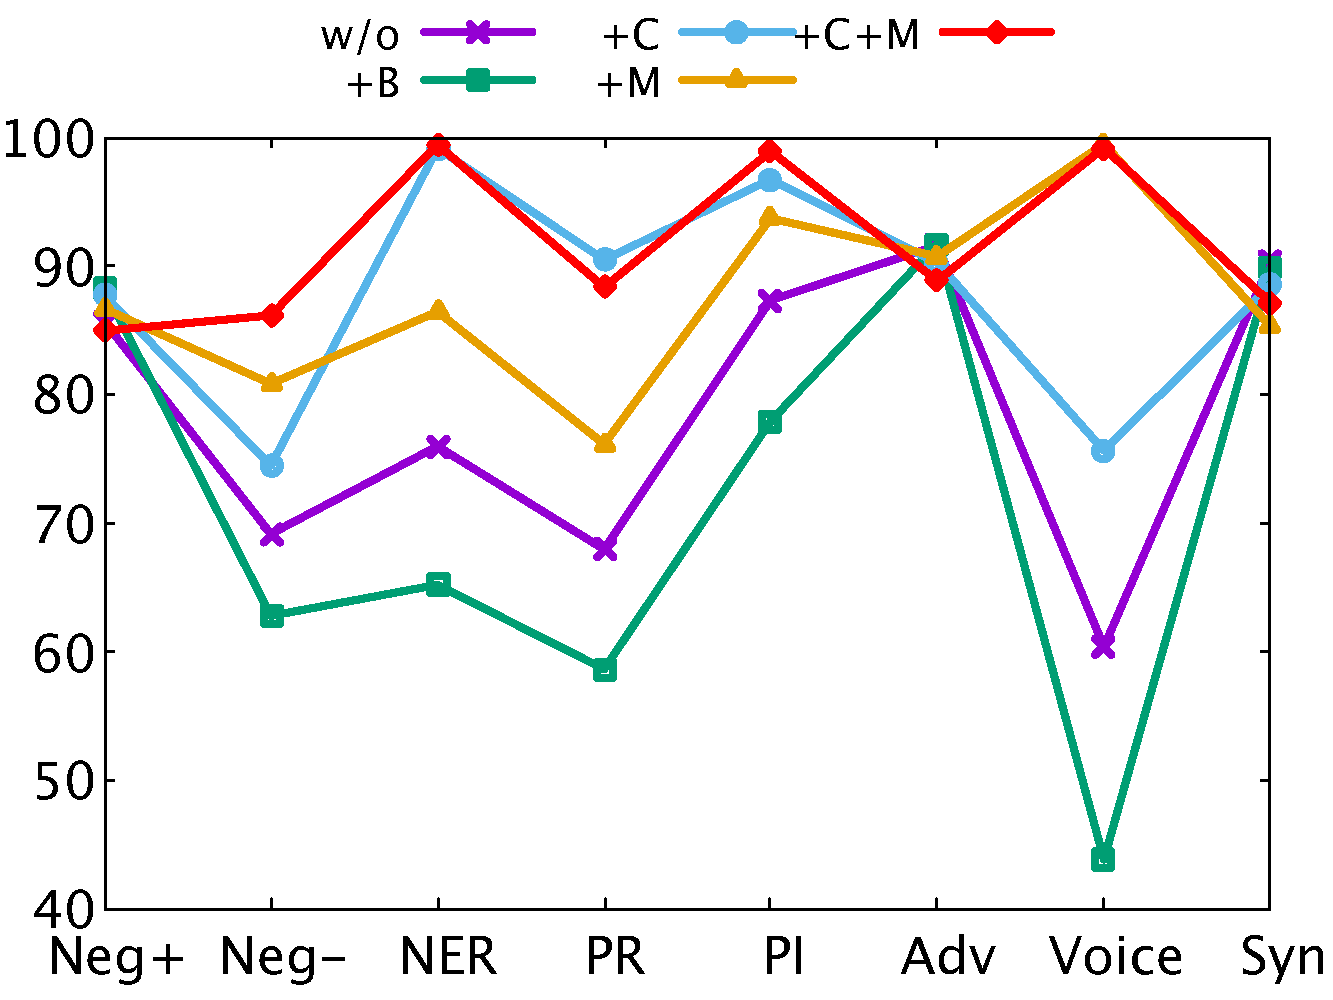
\includegraphics[width=0.6\columnwidth]{data/roc_roberta.pdf}
%   \caption{Detailed stress test with different aspects on ROC dataset. The x-axis indicates different stress test aspects and the y-axis indicates model accuracy in percentage.}
%   \label{fig:detailed}
% \end{figure}


%\begin{figure*}[!th]
%\centering
%\begin{subfigure}[b]{0.28\textwidth}
%\centering
%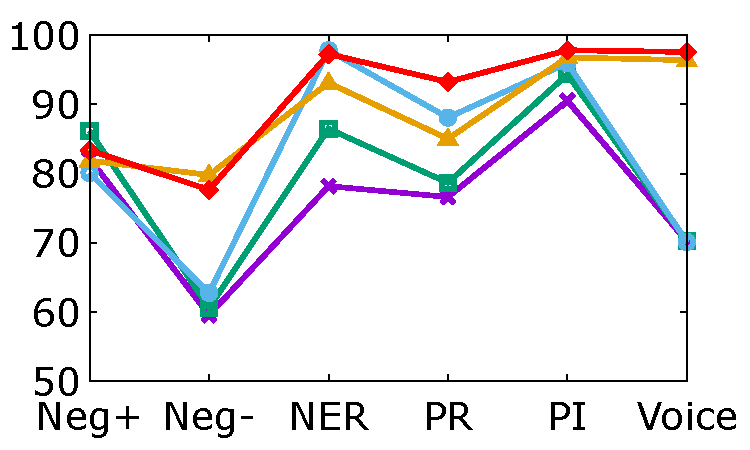
\includegraphics[width=\columnwidth]{data/roc_bert.pdf}
%\caption{BT (ROC)}
%\label{fig:roc_bert}
%\end{subfigure}
%\hfill
%\begin{subfigure}[b]{0.28\textwidth}
%\centering
%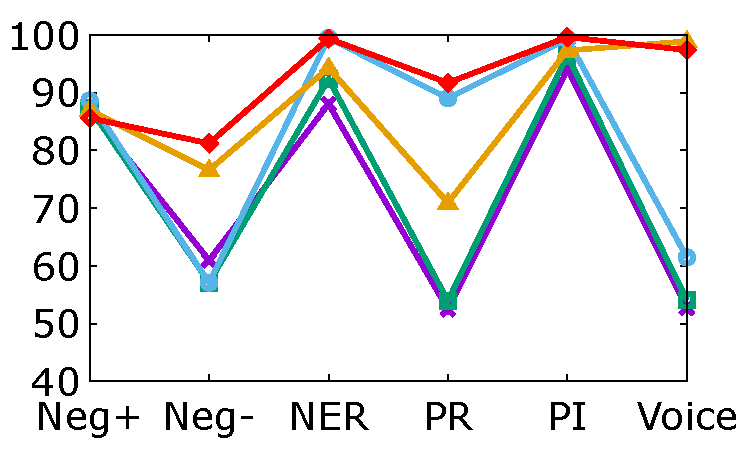
\includegraphics[width=\columnwidth]{data/roc_xlnet.pdf}
%\caption{XL (ROC)}
%\label{fig:roc_xlnet}
%\end{subfigure}
%\hfill
%\begin{subfigure}[b]{0.28\textwidth}
%\centering
%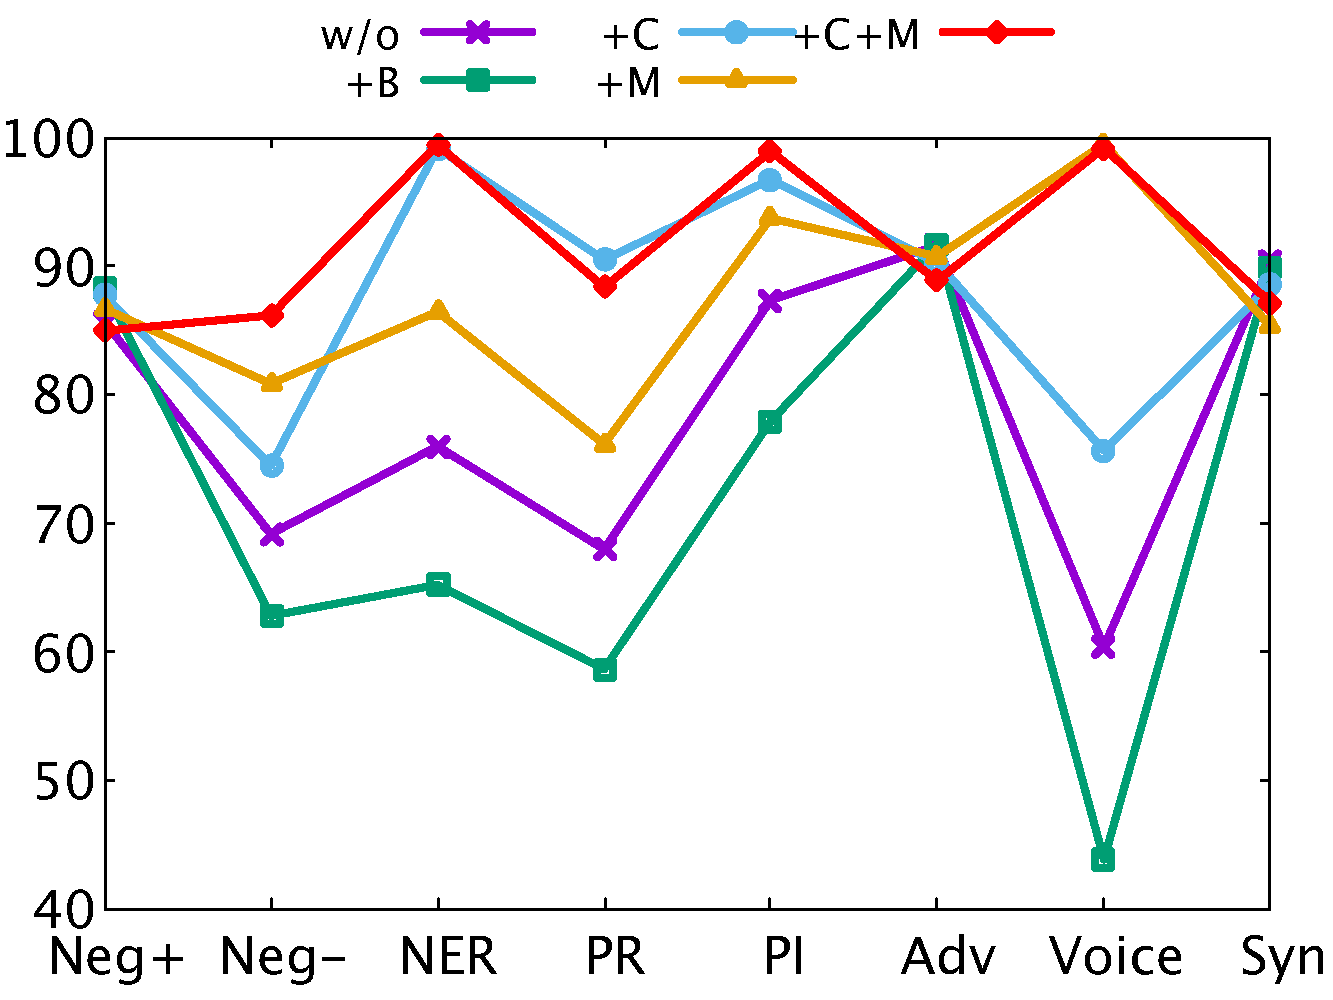
\includegraphics[width=\columnwidth]{data/roc_roberta.pdf}
%\caption{RB (ROC)}
%\label{fig:roc_roberta}
%\end{subfigure}
%\newpage
%\begin{subfigure}[b]{0.28\textwidth}
%\centering
%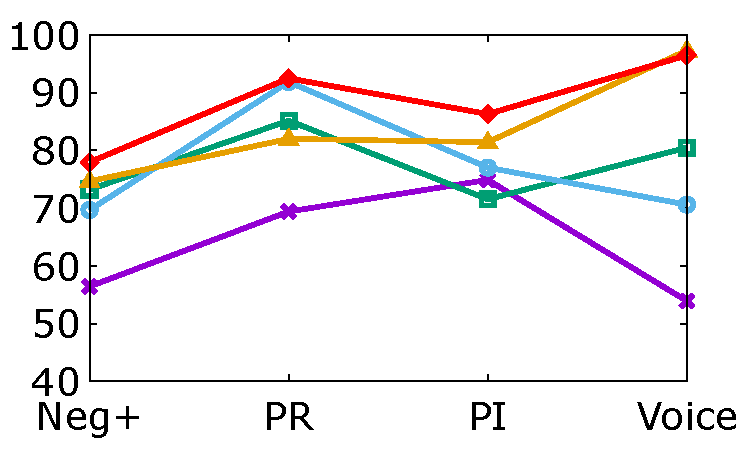
\includegraphics[width=\columnwidth]{data/copa_bert.pdf}
%\caption{BT (COPA)}
%\label{fig:copa_bert}
%\end{subfigure}
%\hfill
%\begin{subfigure}[b]{0.28\textwidth}
%\centering
%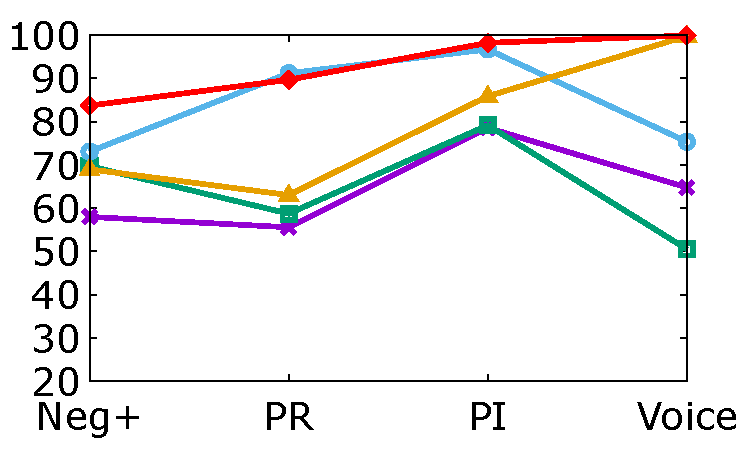
\includegraphics[width=\columnwidth]{data/copa_xlnet.pdf}
%\caption{XL (COPA)}
%\label{fig:copa_xlnet}
%\end{subfigure}
%\hfill
%\begin{subfigure}[b]{0.28\textwidth}
%\centering
%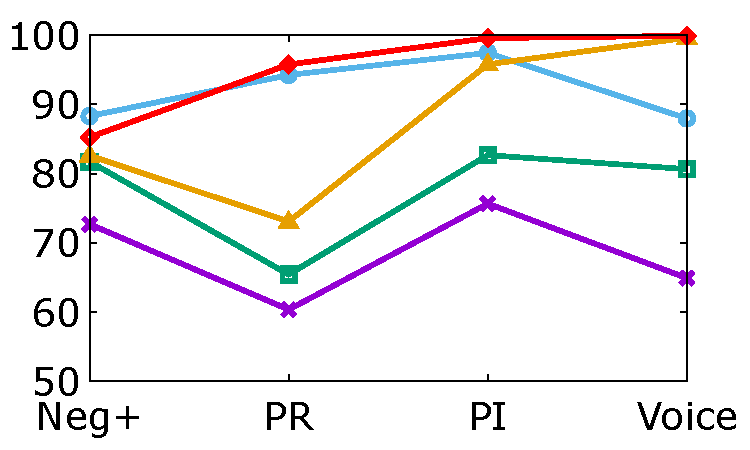
\includegraphics[width=\columnwidth]{data/copa_roberta.pdf}
%\caption{RB (COPA)}
%\label{fig:copa_roberta}
%\end{subfigure}
%\newpage
%\begin{subfigure}[b]{0.28\textwidth}
%\centering
%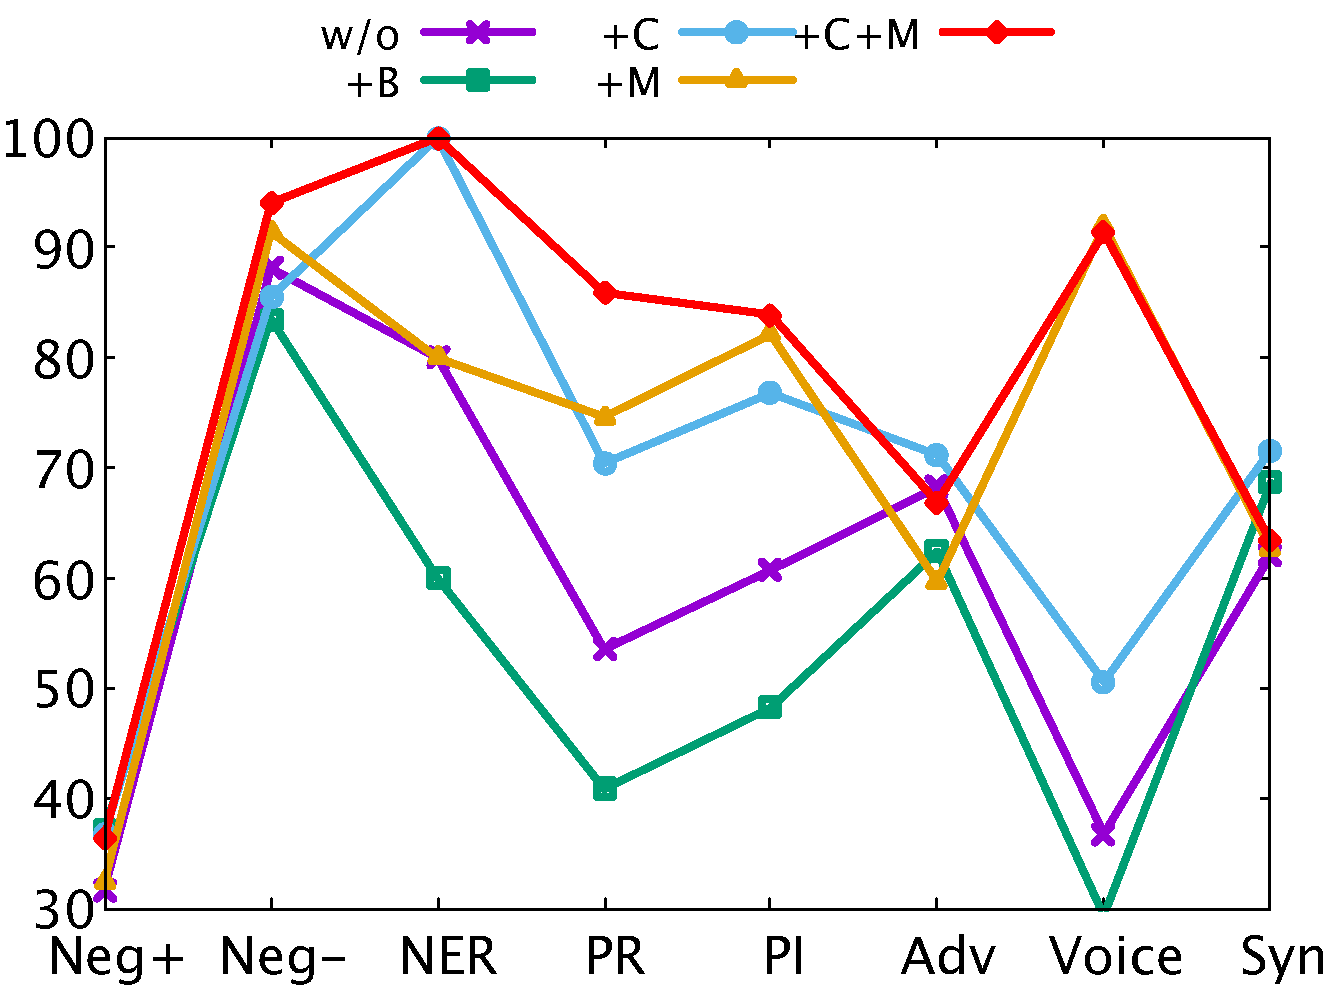
\includegraphics[width=\columnwidth]{data/arct_bert.pdf}
%\caption{BT (ARCT)}
%\label{fig:arct_bert}
%\end{subfigure}
%\hfill
%\begin{subfigure}[b]{0.28\textwidth}
%\centering
%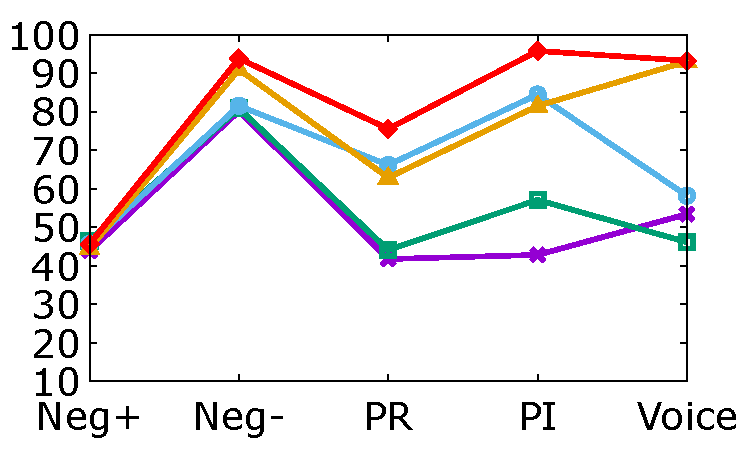
\includegraphics[width=\columnwidth]{data/arct_xlnet.pdf}
%\caption{XL (ARCT)}
%\label{fig:arct_xlnet}
%\end{subfigure}
%\hfill
%\begin{subfigure}[b]{0.28\textwidth}
%\centering
%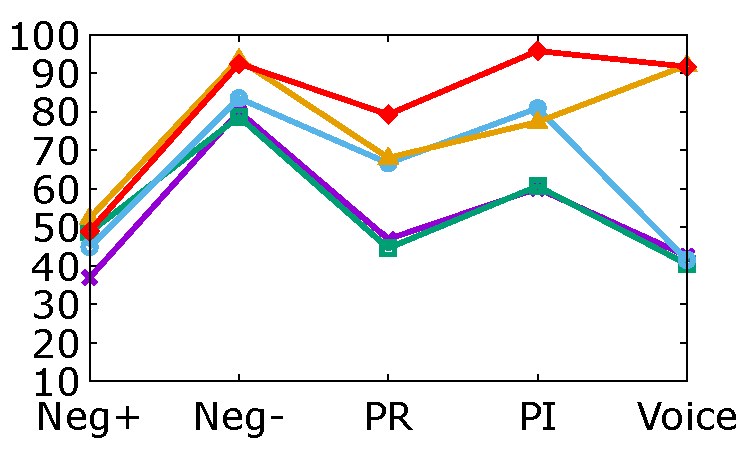
\includegraphics[width=\columnwidth]{data/arct_roberta.pdf}
%\caption{RB (ARCT)}
%\label{fig:arct_roberta}
%\end{subfigure}
%\newpage
%\begin{subfigure}[b]{0.28\textwidth}
%\centering
%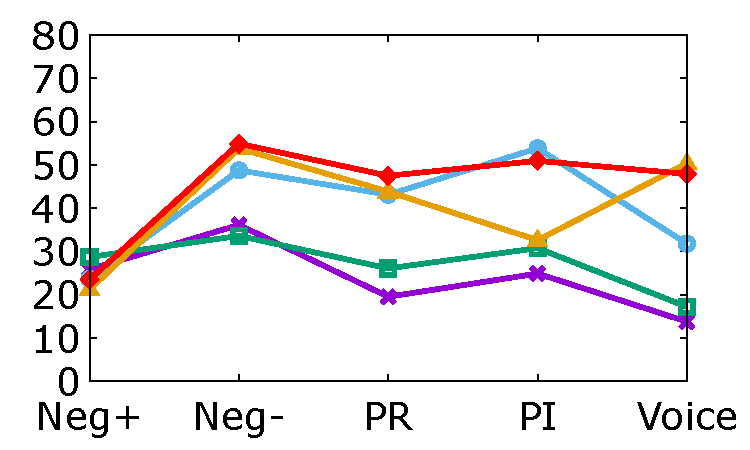
\includegraphics[width=\columnwidth]{data/reclor_bert.pdf}
%\caption{BT (RECLOR)}
%\label{fig:reclor_bert}
%\end{subfigure}
%\hfill
%\begin{subfigure}[b]{0.28\textwidth}
%\centering
%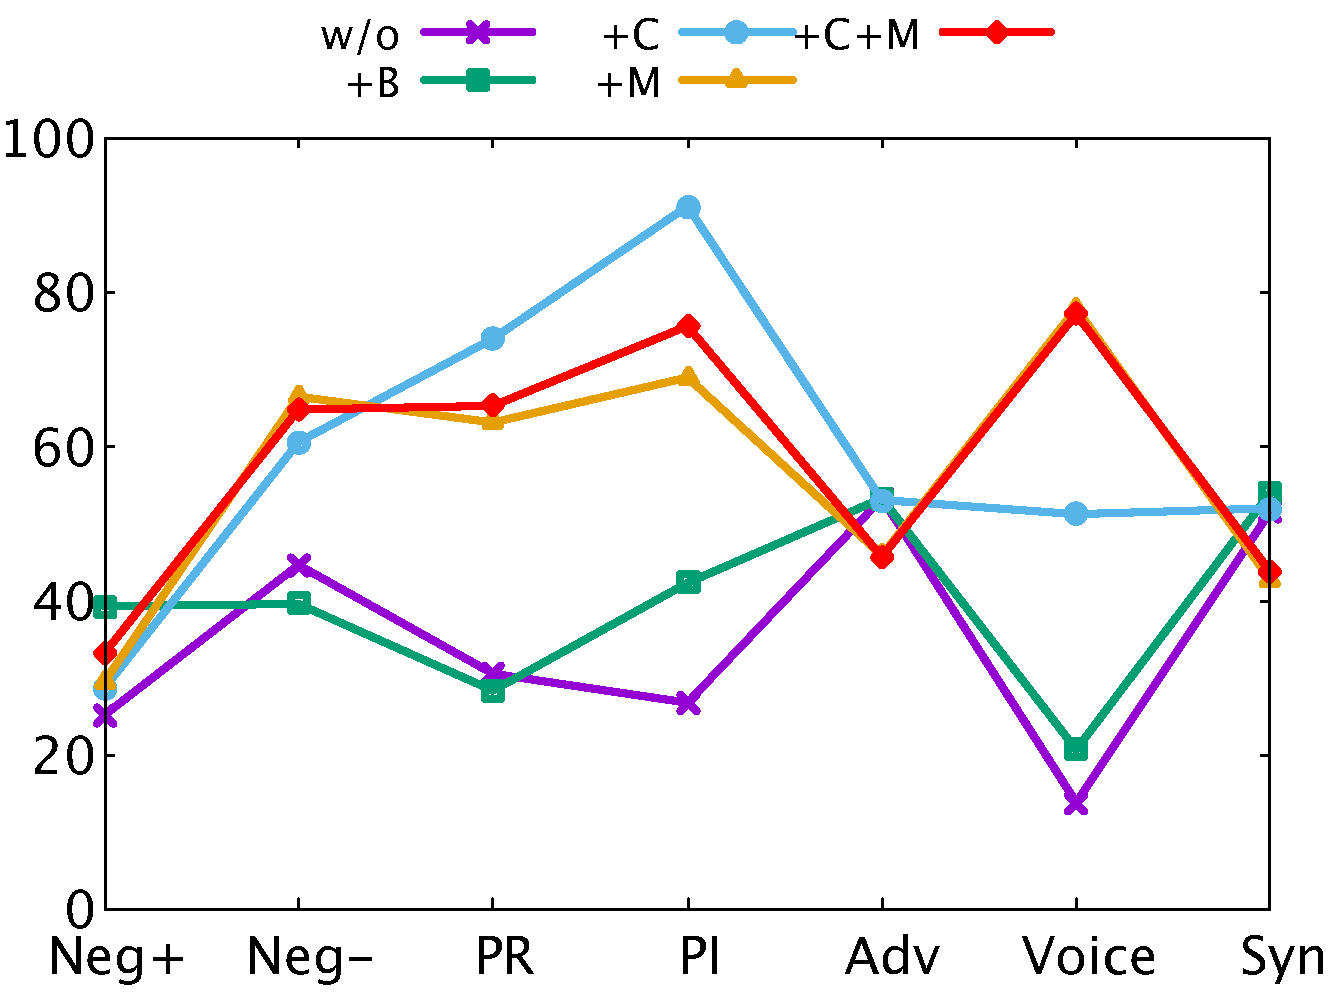
\includegraphics[width=\columnwidth]{data/reclor_xlnet.pdf}
%\caption{XL (RECLOR))}
%\label{fig:reclor_xlnet}
%\end{subfigure}
%\hfill
%\begin{subfigure}[b]{0.28\textwidth}
%\centering
%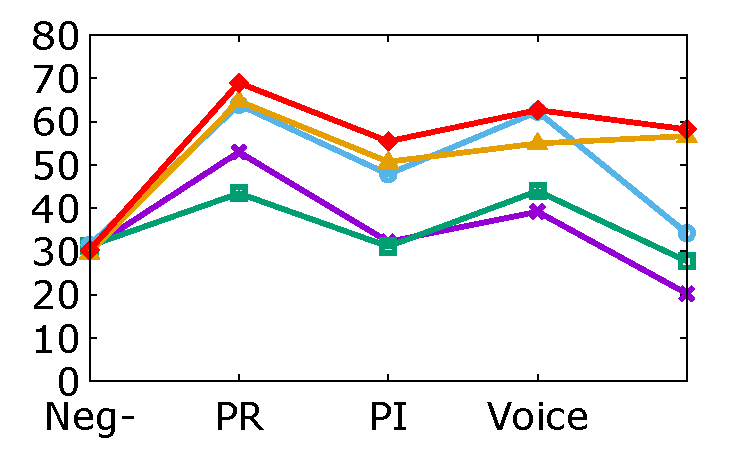
\includegraphics[width=\columnwidth]{data/reclor_roberta.pdf}
%\caption{RB (RECLOR)}
%\label{fig:arct_roberta}
%\end{subfigure}
%\newpage
%\begin{subfigure}[b]{1.0\textwidth}
%\centering
%
\includegraphics[width=0.4\columnwidth]{data/label.jpg}
%\label{fig:label}
%\end{subfigure}
%\caption{Fine-grained stress test with different aspects on 4 different tasks. 
%The x-axis in the figures indicates different stress test aspects and the y-axis indicates model accuracy in percentage.}
%%\KZ{Caption is wrong! most graphs are fine. 
%%But ReCLOR (RB) is a bit strange. 
%%Why is BT line exactly the same as the BT+C? And why is BT+B so bad?}}
%\label{fig:detail}
%\end{figure*}
%%
%
\begin{figure*}[!th]
\centering
\begin{subfigure}[b]{0.24\textwidth}
\centering
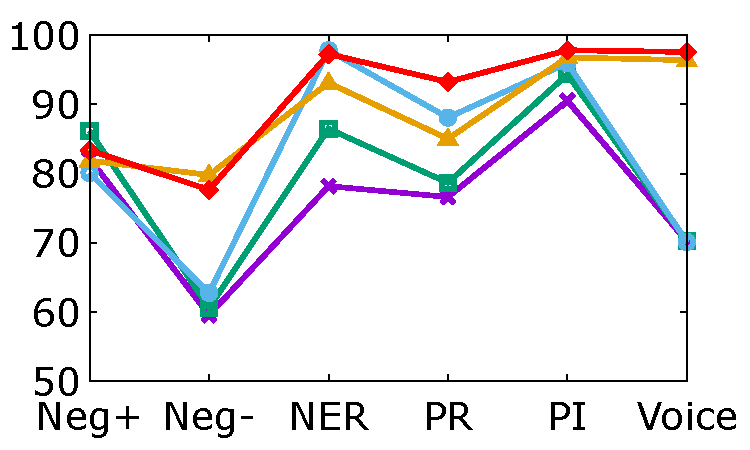
\includegraphics[width=\columnwidth]{data/roc_bert.pdf}
\caption{BT (ROC)}
\label{fig:roc_bert}
\end{subfigure}
\hfill
\begin{subfigure}[b]{0.24\textwidth}
\centering
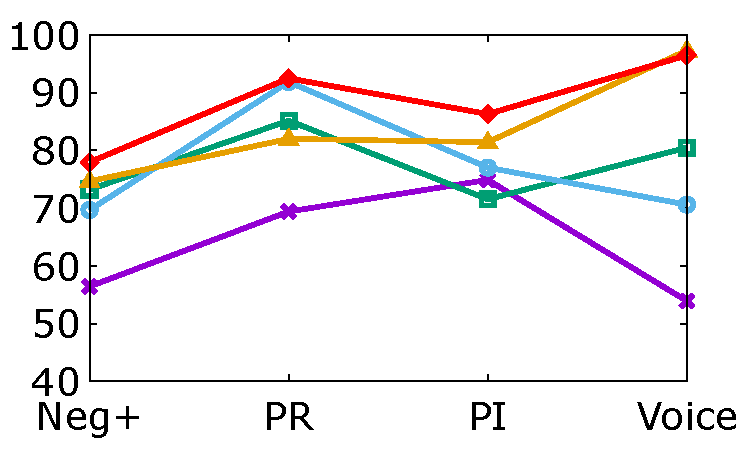
\includegraphics[width=\columnwidth]{data/copa_bert.pdf}
\caption{BT (COPA)}
\label{fig:copa_bert}
\end{subfigure}
\hfill
\begin{subfigure}[b]{0.24\textwidth}
\centering
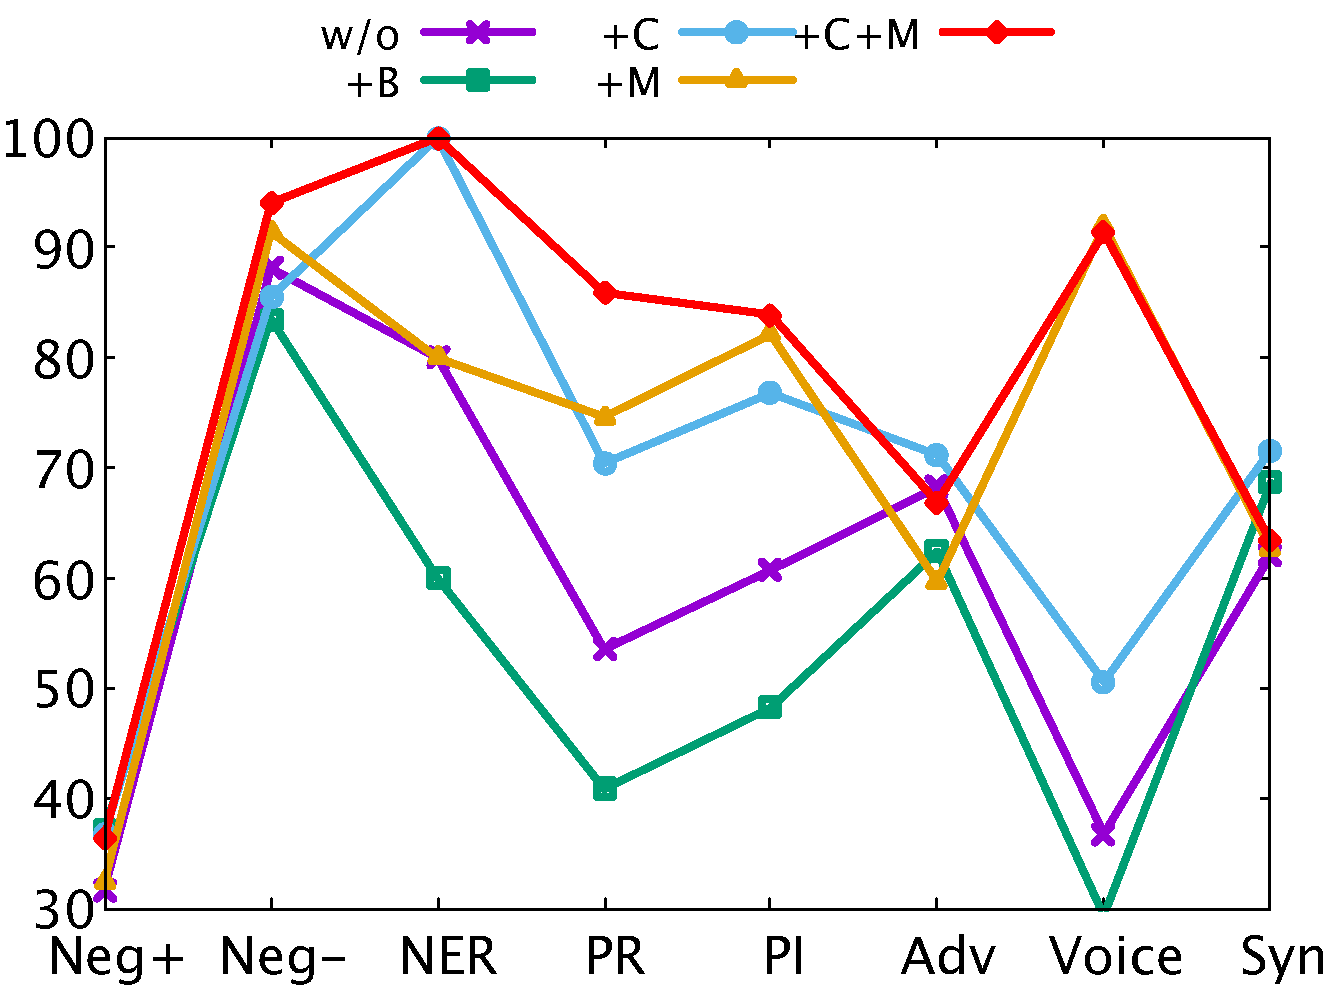
\includegraphics[width=\columnwidth]{data/arct_bert.pdf}
\caption{BT (ARCT)}
\label{fig:arct_bert}
\end{subfigure}
\hfill
\begin{subfigure}[b]{0.24\textwidth}
\centering
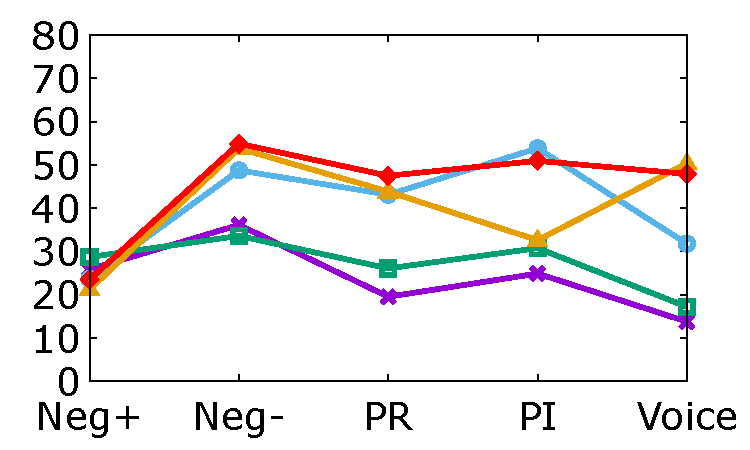
\includegraphics[width=\columnwidth]{data/reclor_bert.pdf}
\caption{BT (RECLOR)}
\label{fig:reclor_bert}
\end{subfigure}
\newpage
\begin{subfigure}[b]{0.24\textwidth}
\centering
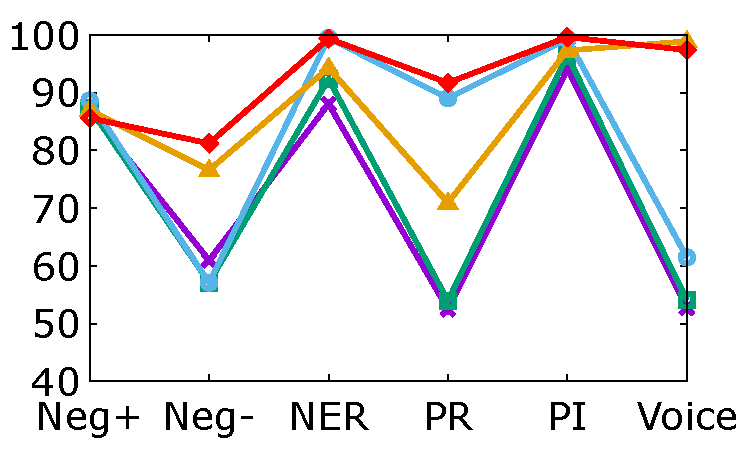
\includegraphics[width=\columnwidth]{data/roc_xlnet.pdf}
\caption{XL (ROC)}
\label{fig:roc_xlnet}
\end{subfigure}
\hfill
\begin{subfigure}[b]{0.24\textwidth}
\centering
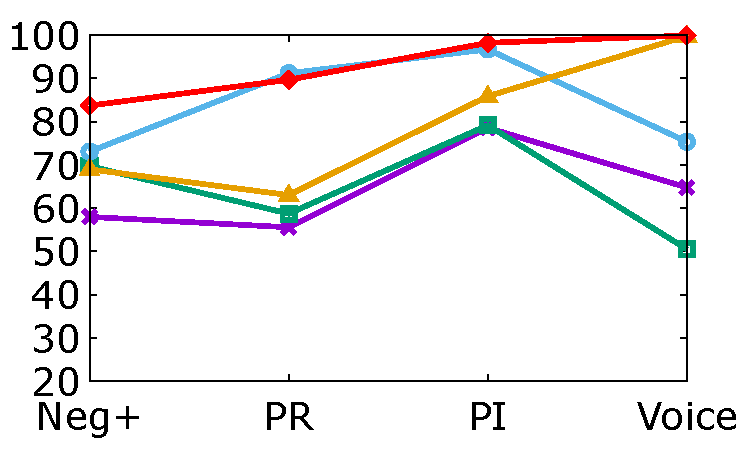
\includegraphics[width=\columnwidth]{data/copa_xlnet.pdf}
\caption{XL (COPA)}
\label{fig:copa_xlnet}
\end{subfigure}
\hfill
\begin{subfigure}[b]{0.24\textwidth}
\centering
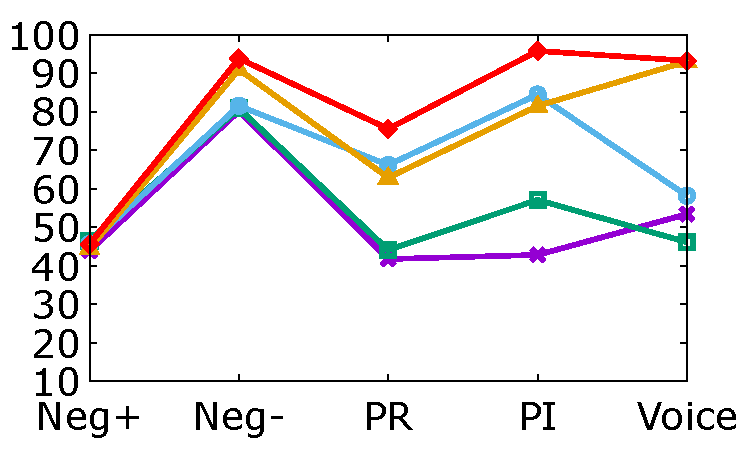
\includegraphics[width=\columnwidth]{data/arct_xlnet.pdf}
\caption{XL (ARCT)}
\label{fig:arct_xlnet}
\end{subfigure}
\hfill
\begin{subfigure}[b]{0.24\textwidth}
\centering
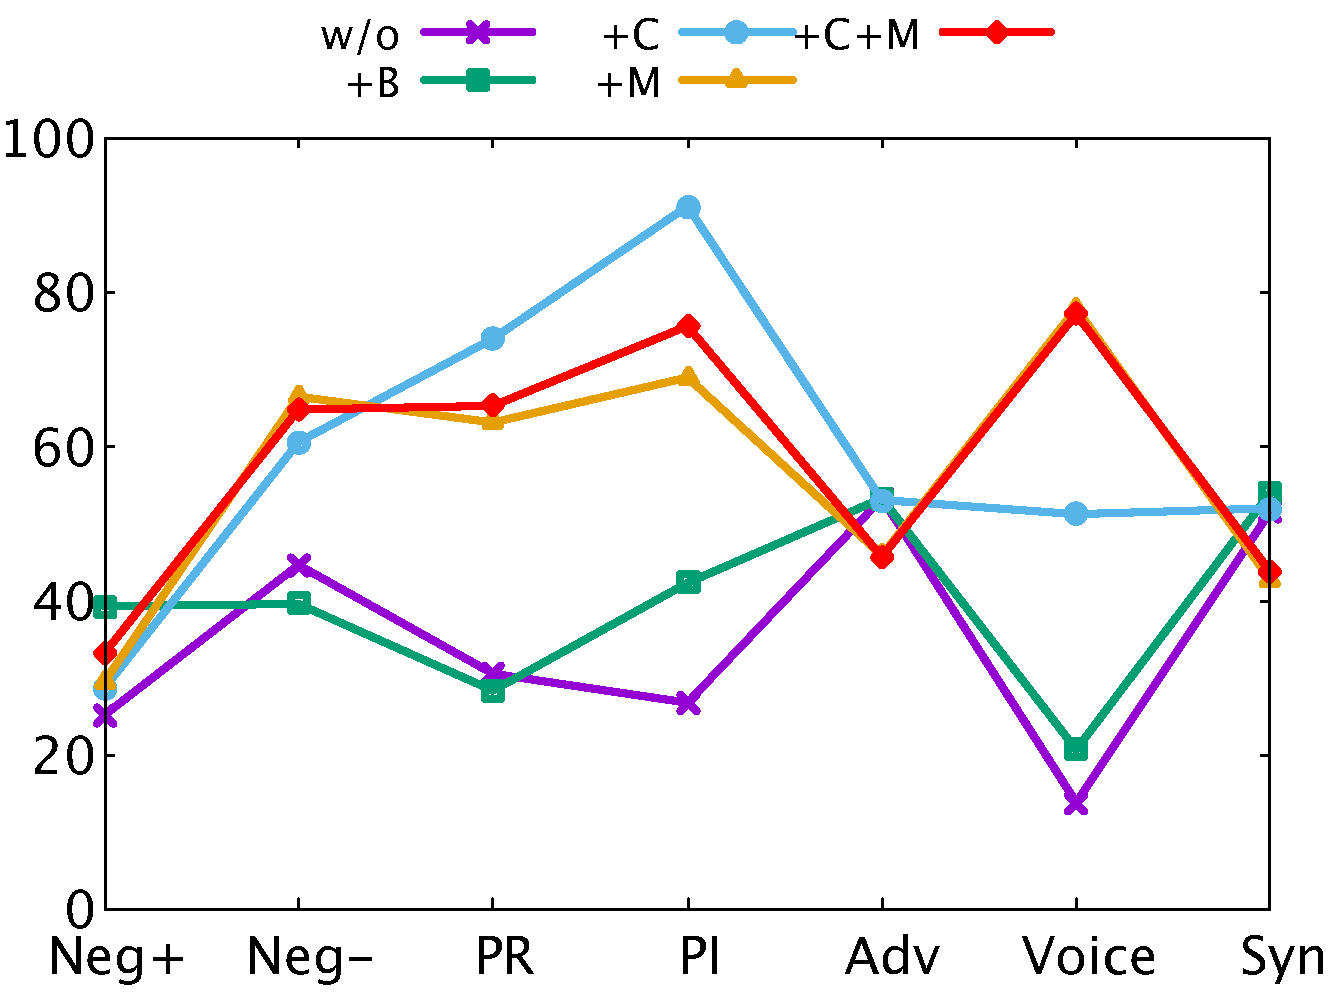
\includegraphics[width=\columnwidth]{data/reclor_xlnet.pdf}
\caption{XL (RECLOR))}
\label{fig:reclor_xlnet}
\end{subfigure}
\newpage
\begin{subfigure}[b]{0.24\textwidth}
\centering
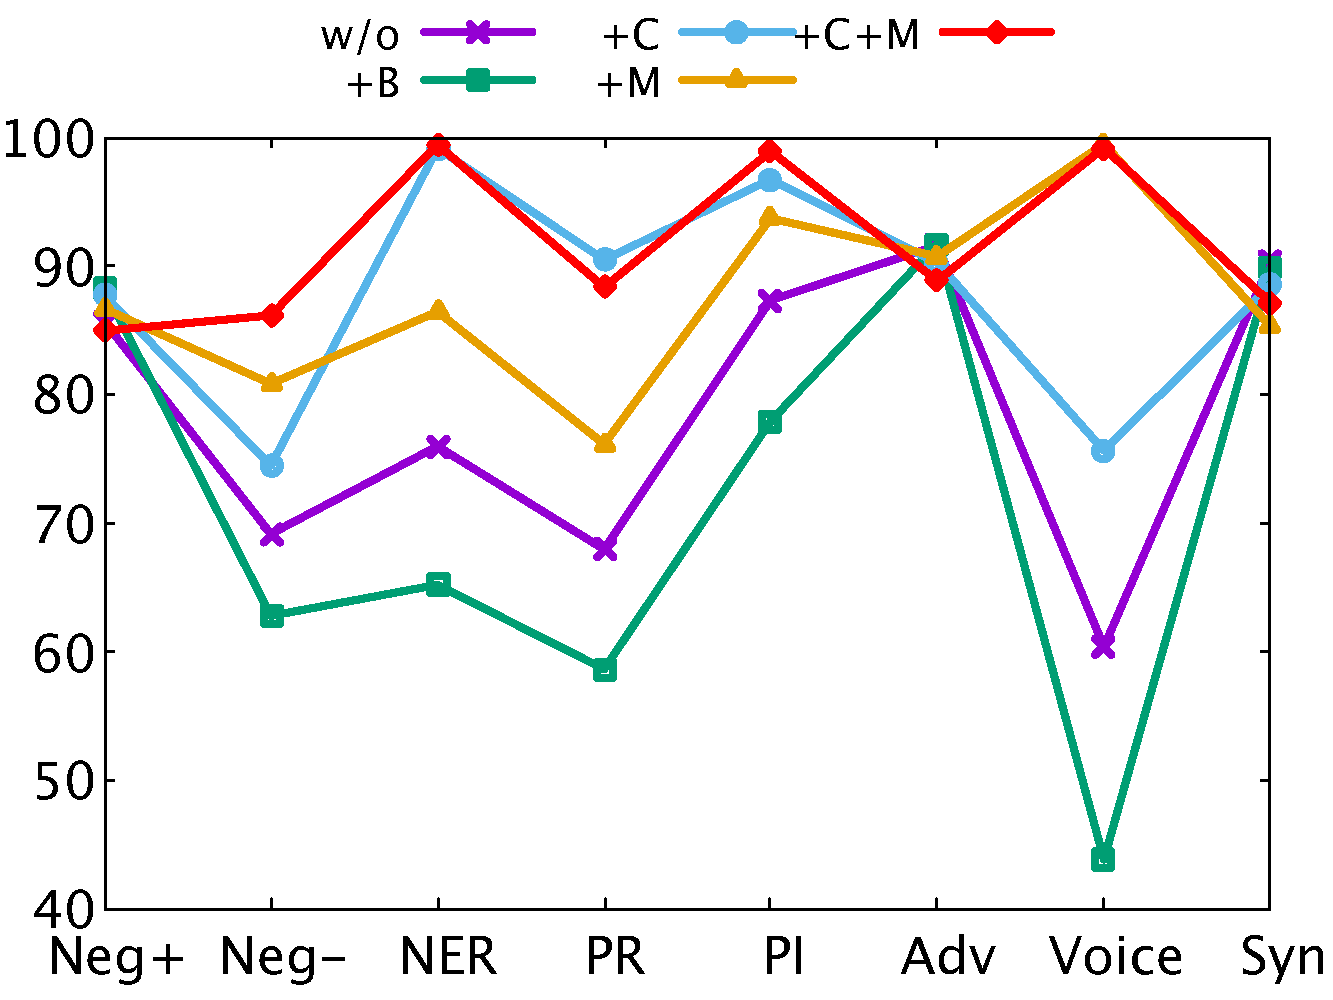
\includegraphics[width=\columnwidth]{data/roc_roberta.pdf}
\caption{RB (ROC)}
\label{fig:roc_roberta}
\end{subfigure}
\hfill
\begin{subfigure}[b]{0.24\textwidth}
\centering
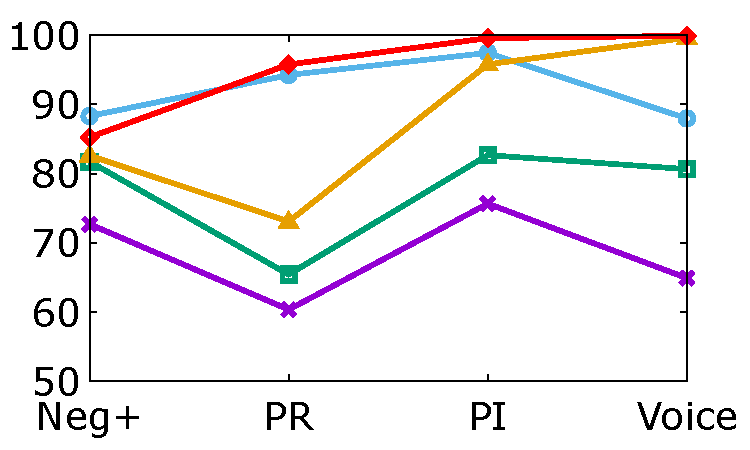
\includegraphics[width=\columnwidth]{data/copa_roberta.pdf}
\caption{RB (COPA)}
\label{fig:copa_roberta}
\end{subfigure}
\hfill
\begin{subfigure}[b]{0.24\textwidth}
\centering
\includegraphics[width=\columnwidth]{data/arct_roberta.pdf}
\caption{RB (ARCT)}
\label{fig:arct_roberta}
\end{subfigure}
\hfill
\begin{subfigure}[b]{0.24\textwidth}
\centering
\includegraphics[width=\columnwidth]{data/reclor_roberta.pdf}
\caption{RB (RECLOR)}
\label{fig:arct_roberta}
\end{subfigure}
\newpage
\begin{subfigure}[b]{1.0\textwidth}
\centering
\includegraphics[width=0.4\columnwidth]{data/label.jpg}
\label{fig:label}
\end{subfigure}
\caption{Fine-grained stress test with different aspects on 4 different tasks. 
The x-axis in the figures indicates different stress test aspects and the y-axis indicates model accuracy in percentage.}
%\KZ{Caption is wrong! most graphs are fine. 
%But ReCLOR (RB) is a bit strange. 
%Why is BT line exactly the same as the BT+C? And why is BT+B so bad?}}
\label{fig:detail}
\end{figure*}
%
\subsubsection{Fine-grained results}
\label{sec:fine-grained}
We proceed to break down the results in \tabref{tab:stressresults} into accuracies on stress tests
created by different operators. 
%We show the detailed results in~\figref{fig:detail} 
%Concretely, six different aspects of stress test data are 
%utilized for testing.
COPA and RECLOR datasets do not show all six operators
because some of the operators generate too little data
for them, as shown in \tabref{tab:cases}. 
%The x-axis in the figures indicates different stress test aspects 
%and the y-axis indicates model accuracy in percentage.
%We apply the proposed two operators \textit{crossover} and \textit{mutation} to BERT, XLNet and RoBERTa 
%models and compare it with back-translation.
%and test on various stress test cases with different aspects. 
The corresponding results are presented in~\figref{fig:detail}. 
We observe that the vanilla model in purple and back-translation in green show
worse results across different aspects than other lines. 
The models trained with data augmented by \textit{crossover} and \textit{mutation} 
(the red lines) are generally more robust than others.
%\KZ{It is consistent with our overall results in~\tabref{tab:results}.} 
Please refer to Appendix A. 
%\footnote{There are some dashes in the table because the } 
for complete results. 
%\KZ{You need to explain why there are some dashes in the table in appendix.}

%We also observe that the 
%accuracy performance points for ``Syn'' and ``Adv'' are concentrated 
%but scattered on other operator aspects. 
Since every type of stress tests 
%(except ``Syn'' and ``Adv) 
can evaluate if a model is robust, particularly if it considers the 
premise by giving it two very similar choices, 
the above results on the stress tests of all types show that our two methods do 
%improves the model robustness, and may even encourage the models to look toward the
reduce short-circuits, and may even encourage the models to look toward the
premises.
We will provide additional pieces of evidence to confirm this in the next two subsections.

%\KZ{The weakness can be on the same table as the improvements
%to save space.}
%\KZ{Check the following analysis to make sure it's consistent with the tables.}

%Compared with 
%base models without data augmentation, we find that 
%all four data augmentation methods moderately improve
%the models when tested on the original test set. 
%In ROC, accuracy of BERT and RoBERTa trained with crossover augmented data 
%exceeds base models and ranks top. Crossover method also works on COPA. 
%Even though back-translation obtains higher score mostly on ARCT and RECLOR,
%crossover, mutation and crossover+mutation barely fall below the base model. 
%
%Augmentation fares much better in the ``Stress'' columns, though
%different methods show varying degree of success.
%Compared with the model without data augmentation, 
%the performance of models with crossover 
%has always been greatly improved (i.e., by 21.44\% for BERT on COPA).
%It indicates that reducing the short circuits 
%is a good way to improve the robustness of a model.
%The performance of new models with crossover has 
%great improvement for all models on different dataset 
%compared with the model without data augmentation, like 21.44% for BERT on COPA. 
%Mutation alone can also help with robustness on stress test better than crossover.
%This result suggests that mutation is a good method 
%for enhancing the robustness of models. 
%Though, mutation may be not a 
%good method to decrease the short circuits (\secref{sec:fix-sc}). 
%Overall, crossover+mutation 
%can mostly get the best performance on the stress test except for 
%training on RECLOR with RoBERTa. 
%to This result indicates that this kind of data can prevent models from being confused 
%by simple perturbations thus improving the robustness of models. 
%Besides, we can also find that back-translation doesn't improve the models' robustness much.
%Crossover alone can also help with robustness on stress test but 
%no better than mutation and crossover+mutation.  

%some of Table 5's AW scores being 
%some of Table 5's AW scores being 
%lower than AW for model w/o augmentation (e.g., 45.13 in (b)), 
%then the reason is AW is only a proxy test
%that catches majority of short circuit cases in our opinion, 
%but it's not perfect, as we pointed out in A2 of R1. 
%If you are referring to some accuracies in the Original columns 
%being lower than models w/o augmentation in Table 5 (e.g., 72.6 in (b)), 
%the reason is some models w/o augmentation might have 
%"cheated" to get high accuracy. Augmenting (C or M) corrects the
%biases in these models and may reduce the accuracy on the original test set.
%Nevertheless, all models after augmentation do better on the stress tests.

%have least short circuits based on BERT and XLNet. 
%Crossover+mutation based on RoBERTa takes less short circuits than others. 
%In the CO and AW columns, the result are consistent on ROC. 

%\subsection{White-box Attention Weights~(AW)}
%\KZ{Here we first talk about human testing by visualizastion,
%then talk about how to automatic it thru code.}

%show human annotation results of bert, roberta, xlnet.
%For exploiting whether attention-based models are suffered from short circuits, 
%we propose to 
%use the AW method which we have described in~\secref{}.
%It is noted that t\_1 is greater than t\_2. 
%Here t\_1 and t\_2 are tuned to 0.14 and 0.13 separately.

\subsection{Choice-only Test}
\label{sec:choice-only}

%In this section, we use choice-only test for different models on four tasks. 
%We have shown the effectiveness of \textit{crossover} and \textit{mutation} on in robustness test. 
The end-to-end test has shown the success of our data augmentation 
methods. To further explore the reason behind the performance gain, 
we also use choice-only test here.

%somewhat confirm the reason for model improvement with data augmentation 
%strategies. Moreover, this test is used to further explore 
%whether our strategies can encourage models pay more attention to premise.
In choice-only test, we only feed choices into a model without a premise which is replaced 
by an empty string. This way, 
models cannot utilize the relationship between premise and choices. 
%what we can know whether a model can 
%solve cases easily without awaring premise by test accuracy. 
Normally, we would expect the model to make arbitrary choices.
However, if a model can easily ``guess'' the ``right'' choice which 
normally requires the relationship between premise and choices,  
one possibility is that this model cheats on evaluation procedure and 
may be fragile. Thus, the higher score may indicate more use of short-circuits.

In~\figref{fig:choice-only}, we observe that in choice-only tests,
the accuracy of models augmented with \textit{crossover} and \textit{mutation} 
(red line) drops the most. 
Sometimes the performances are similar to random selection, e.g., 
RB+C+M on ARCT (56.38\%), which indicates that models 
are no longer cheating. 
In other words, models augmented by crossover and mutation 
are more likely to consider the premises. 
The results on the choice-only tests provide another perspective for us
to re-assure that models augmented with crossover and mutation can reduce
short circuits and thus model fragility.

%\KZ{Rephrase: 
%However, another possibility reason for lower choice-only test accuracy 
%that is also not ruled out is that 
%even if the model can tell the result with only choices, 
%it still chooses to look at the premise context. 
%Although high scores do not necessarily imply models 
%are not looking forward, low scores necessarily mean that models cannot 
%conclude that solely relying on choices.} 

%\begin{table}[th]
%\centering
%\scriptsize
%\begin{tabular}{c|rrrr}
%\toprule
%\textbf{Model} & \textbf{ROC} & \textbf{COPA} & \textbf{ARCT} & \textbf{RECLOR} \\ \midrule
%%BT  &98.76 &89.68&\textbf{99.65}&82.46    \\ \hline
%%BT+B  &99.26 &96.79   &99.34  &86.01  \\ \hline
%%BT+C  &\textbf{99.69} &\textbf{98.35}&98.37   &80 \\ \hline
%%BT+M  &99.26 & 95.17 &98.67 &82.48    \\ \hline
%%BT+C+M  &98.82 &96.96 &98.00 &\textbf{96.79}  \\ \midrule
%%XL  &28.08 &93.16 & 85.67 & 79.64 \\ \hline
%%XL+B  &19.27  &91.46 &95.73 & 81.40   \\ \hline
%%XL+C  &\textbf{64.58} &45.13  &55.59  &\textbf{87.87} \\ \hline
%%XL+M  &62.77  &96.85 & \textbf{95.74}& 72.76  \\ \hline
%%XL+C+M  &60.25 & \textbf{98.51}&86.26 &   48.71\\ \midrule
%%RB  &77.41 & 80.89 & 99.14& 85.88 \\ \hline
%%RB+B  &   58.15 &\textbf{96.36}   & 97.78& 15.69  \\ \hline
%%RB+C  &   82.71& 89.62&79.19& 89.68\\ \hline
%%RB+M  &71.73& 62.26& \textbf{100.00}&\textbf{100.00}  \\ \hline
%%RB+C+M  &\textbf{93.31} &61.89    &71.47 & 89.26\\ 
%%
%BT (w/o)&54.62&51.4&61.94&42.8 \\ \hline
%BT+B&58.26&50.8&64.41&39.2  \\ \hline
%BT+C&51.2&48.2&55.63&30.8  \\ \hline
%BT+M&51.79&48.8&55.18&38   \\ \hline
%BT+C+M&43.56&49.4&52.03&33.8  \\ \midrule
%XL (w/o)&71.14&57&65.99&42.2 \\ \hline
%XL+B&73.17&60&66.89&41.4  \\ \hline
%XL+C&65.63&55&55.86&34.2  \\ \hline
%XL+M&71.94&57.8&66.22&42  \\ \hline
%XL+C+M&66.22&58.4&62.84&35  \\ \midrule
%RB (w/o)&73.97&59.4&67.79&30.2 \\ \hline
%RB+B&74.77&61.4&69.37&42.2  \\ \hline
%RB+C&73.06&58.4&68.47&34.6  \\ \hline
%RB+M&70.34&56&61.49&40      \\ \hline
%RB+C+M&71.3&54.8&67.79&32.2  \\ 
%\bottomrule
%\end{tabular}
%\caption{Choice-only test for transformer-based models on 4 datasets. All numbers are percentages (\%)}
%%\KZ{I assume this is the ending-only test? But isn't scriptsizeer the better
%%for ending-only tests?}}
%\label{tab:only-test}
%\end{table}
%
\begin{figure}[th]
    \centering
    \includegraphics[width=0.7\columnwidth]{data/choice-only.pdf}
    \caption{Choice-only test: Accuracies of different data augmentation methods with 3 models on 4 tasks. 
    The detailed numbers are in Appendix B.}
    \label{fig:choice-only}
\end{figure}

However, one may argue that even if a model can 
choose or ``guess'' correctly given only the choices but no premise, 
it may still have the ability to look at the premise if it's given one,
like in the end-to-end test.
Therefore, next we conduct an additional case study to show that short-circuit
does take place and our augmentation methods alleviate it.

\subsection{Case Study}
\label{sec:case}

%\begin{figure}[th!]
%\centering
%\begin{subfigure}[b]{0.21\textwidth}
%\centering
%
%\framebox{\includegraphics[width=\columnwidth]{figure/case_original.eps}}
%\caption{RB(w/o)}
%\label{fig:case_original}
%\end{subfigure}
%\hfill
%\begin{subfigure}[b]{0.21\textwidth}
%\centering
%\framebox{\includegraphics[width=\columnwidth]{figure/case_b.eps}}
%\caption{RB+B}
%\label{fig:case_b}
%\end{subfigure}
%\hfill
%\newpage
%\begin{subfigure}[b]{0.21\textwidth}
%\centering
%\framebox{\includegraphics[width=\columnwidth]{figure/case_c.eps}}
%\caption{RB+C}
%\label{fig:case_c}
%\end{subfigure}
%\hfill
%\begin{subfigure}[b]{0.21\textwidth}
%\centering
%\framebox{\includegraphics[width=\columnwidth]{figure/case_cm.eps}}
%\caption{RB+C+M}
%\label{fig:case_cm}
%\end{subfigure}
%\caption{Attention map on a COPA example for models.}
%%\KZ{Caption is wrong! most graphs are fine. 
%%But ReCLOR (RB) is a bit strange. 
%%Why is BT line exactly the same as the BT+C? And why is BT+B so bad?}}
%\label{fig:case}
%\end{figure}
%

%In \figref{fig:case}, 
%%illustration. There is no positive attention value in front of the 
%%fourth sentence, so we intercept it from where it is worth. 
%RoBERTa trained on the original training set fails to pick up the 
%relation between ``pushed'' and ``opened''. 
%%right choice likely due to there being virtually no attention 
%%connection between words in the choice and words in the premise. 
%After training with \textit{crossover} data augmentation, 
%the model learns to build contextual reasoning  
%by attending to relevant concepts in the premise. 
%%i.e., ``show'' in this example. The rationale behind 
%%such a change of attention pattern is that, 
%%in a MCQ created by crossover operation, 
%%the model needs to combine information 
%%in the premise to effectively 
%%distinguish the true ``right'' choice from the wrong one, 
%%which is also a right choice in another MCQ. 
%to have not enhanced such abilities. We provide additional cases in Appendix C.

%\begin{figure}[th]
%\centering
%{\setlength{\fboxsep}{0pt}
%5\framebox{%
%\includegraphics[width=0.47\columnwidth]{figure/o_un.eps}
%}
%\hfill
%\framebox{%
%\includegraphics[width=0.47\columnwidth]{figure/cross_un.eps}
%}
%}
%\caption{Attention maps showing that RoBERTa short-circuits on a ROC
%question (left) and no longer short-circuits after data augmentation (right). \KZ{I suggest we show a few more cases here to be more convincing. Show the before and after. Before there's no attention to the
%premise, after there is.}}
%\label{fig:case_study}
%\end{figure}

%\begin{example}\label{ex:roc}
%An MCQ from ROC:\\ \\
%\noindent
%\textbf{Premise:} Sarah was home alone. She wanted to stay busy. She turned on the TV. 
%She found a reality show to watch.  \\
%\textbf{Choice 1:} Sarah then happily watched the show.  \checksymbol  \\
%\textbf{Choice 2:} Sarah could not find anything to watch. \crosssymbol
%\end{example}

Our case study is a series of white-box tests that demonstrate
the change in attention patterns.

We take an example from ROC which is shown in~\tabref{table:dataset}.
We explore BERT-based models by 
analyzing their attention maps on this case in~\figref{fig:roc_bert}.  
In this example, the word ``show'' in the premise is strongly
related to the token ``reality show'' in the right choice from human knowledge. 
%The relationship between these two words is the key to answering this question. 
%We explore different models with the augmentation method with attention map 
%to visualize if these two words have a relationship or not.
The attention map is visualized via an off-the-shelf tool~\cite{vig-2019-multiscale}.


There is no positive attention value in front of the fourth sentence, 
so we intercept it from where it is worth. 
BERT trained on the original training set fails 
to pick up the right choice likely due to there being 
virtually no attention connection between words in 
the choice and words in the premise.
After training with \textit{crossover} data augmentation, 
the model learns  
to pay attention to the premise and the relationship 
between premise and choices. 
i.e., ``show'' in this example. 
Similar trends also exist for the \textit{mutation} operation in \figref{fig:roc_m} 
and the combination of \textit{crossover} 
and \textit{mutation} operation in~\figref{fig:roc_cm}. 
The rationale behind 
such a change of attention pattern is that, 
in an MCQ created by \textit{crossover} operation (\figref{fig:roc_c}), \textit{mutation}(\figref{fig:roc_m}), 
and the combination of them (\figref{fig:roc_cm}), 
the model needs to combine the information 
in the premise to effectively 
distinguish the true ``right'' choice from the wrong one. 
However, the light and sparse attention color blocks on the attention map for back-translation 
in \figref{fig:roc_b} indicate back-translation 
can not help BERT connect the choice and premise very well in this question.
These observations empirically demonstrate the effectiveness of our methods 
in encouraging the model to pay attention to the premise to reduce 
short circuits. We provide additional cases in Appendix C. 

%\begin{figure}[th!]
%\centering
%\begin{subfigure}[b]{0.35\textwidth}
%\centering
%\framebox{\includegraphics[width=\columnwidth]{figure/roc_b.eps}}
%\caption{BT+B}
%\label{fig:roc_b}
%\end{subfigure}
%\hfill
%\begin{subfigure}[b]{0.35\textwidth}
%\centering
%\framebox{\includegraphics[width=\columnwidth]{figure/roc_c.eps}}
%\caption{BT+C}
%\label{fig:roc_c}
%\end{subfigure}
%%\hfill
%\newpage
%\begin{subfigure}[b]{0.35\textwidth}
%\centering
%\framebox{\includegraphics[width=\columnwidth]{figure/roc_m.eps}}
%\caption{BT+M}
%\label{fig:roc_m}
%\end{subfigure}
%\hfill
%\begin{subfigure}[b]{0.35\textwidth}
%\centering
%\framebox{\includegraphics[width=\columnwidth]{figure/roc_cm.eps}}
%\caption{BT+C+M}
%\label{fig:roc_cm}
%\end{subfigure}
%\caption{Attention map on a ROC example for BERT-based models.}
%%\KZ{Caption is wrong! most graphs are fine. 
%%But ReCLOR (RB) is a bit strange. 
%%Why is BT line exactly the same as the BT+C? And why is BT+B so bad?}}
%\label{fig:roc_bert}
%\end{figure}
%
\begin{figure}[h!]
\centering
\begin{minipage}{0.30\linewidth}
    \centering
    \fbox{\includegraphics[width=\linewidth]{figure/roc_b.eps}}
    \caption*{BT+B}
    \label{fig:roc_b}
\end{minipage}
\hspace{0.5cm}
\begin{minipage}{0.30\linewidth}
    \centering
    \fbox{\includegraphics[width=\linewidth]{figure/roc_c.eps}}
    \caption*{BT+C}
    \label{fig:roc_c}
\end{minipage}
\hspace{1.5cm}
\vspace{0.5cm}
\begin{minipage}{0.30\linewidth}
    \centering
    \fbox{\includegraphics[width=\linewidth]{figure/roc_m.eps}}
    \caption*{BT+M}
    \label{fig:roc_m}
\end{minipage}
\hspace{0.5cm}
\begin{minipage}{0.30\linewidth}
    \centering
    \fbox{\includegraphics[width=\linewidth]{figure/roc_cm.eps}}
    \caption*{BT+C+M}
    \label{fig:roc_cm}
\end{minipage}
\caption{Attention map on a ROC example for BERT-based models.}
\label{fig:roc_bert}
\end{figure}


%\subsection{Discussion}
%
%From previous test results on original test, stress test, choice-only test and test cases analysis, 
%we can illustrate that \textit{crossover} and \textit{mutation} can teach models to pay more attention to 
%the relationship between the premise and the choices. However, there is a doubt that \textit{mutation} 
%can triger a new bias cue that once the model find the choice is ingrammatically, it will choose another 
%choice. 
%%Thus we make another experiment to verify whether the augmentation operator \textit{mutation} can 
%Thus in this section, we make an experiment that we generate new grammar test cases which only 
%mutate words in the right choices. If models' prediction results are unchanged, 
%it can indicate that these models which trained with augmentation 
%data can't be easily triggered by the grammatical cues. The test result for models are shown in \tabref{tab:mutate} on ROC dataset. 
%We can find that the predicting change rate for +M models are not higher than vanilla models which illustrates 
%that +M will not introduce extra grammatical bias cues.
%\begin{table}[th!]
%   \centering
%   \scriptsize
%   \begin{tabular}{lc}
%       \toprule
%       \textbf{Model}& Change Rate \\
%       \midrule
%       BT(w/o)& 7.35\\
%       BT+M&6.37\\
%       \midrule
%       XL(w/o)&8.17 \\
%       XL+M&8.45 \\
%       \midrule
%       RB(w/o)&5.94\\
%       RB+M&5.73\\
%       \bottomrule
%   \end{tabular}
%   \caption{Grammatical sensitivity test on ROC dataset. All the numbers are percentage(\%)}
%   \label{tab:mutate}
%\end{table}




\section{Analysis}


For a better understanding of ICL-SC, 
we did comprehensive ablation studies and combined it with the traditional CL. The experiments in this section are done on dialogue summarization, which is representative due to the medium output length.




\subsection{Ablations on the Training Strategy}

%1. strategy: increase; decrease; random
To examine the design of decreasing the prefix for ICL-SC, we introduce the ablation of training strategies as follows:
\begin{itemize}
	\item \textbf{Decrease} refers to the Algorithm~\ref{alg:picl}. Taking $p_{start}=0.6$ and $s=0.3$ as an example, the prefix percentage $p$ varies as $0.6\rightarrow 0.3\rightarrow 0.0$ during training.
	\item \textbf{Increase} means that we gradually increase the length of prefix by increase $p$ following $0.0\rightarrow0.3\rightarrow0.6$.
	\item \textbf{Random} is that we randomly pick $p$ from the set $\{0.0, 0.3, 0.6\}$ in this example.
\end{itemize}

The results are shown in Table~\ref{tab:ablstrategy}, with Decrease ranking first and Increase ranking the worst.
Decrease significantly outperforms other ablations, showing that our sequence completion criterion of shrinking the prefix does work by means of learning from easy to hard.
%, instead of the implicit ``data augmentation'' which calculates different losses given the same sample during training.

\begin{table}[th]
	\scriptsize
	\centering
	\begin{tabular}{cccccc}
		\hline
		{Stra.} & {R1} & {R2} & {RL} & {Met} & {BertS} \\
		\hline
		Decrease &\textbf{53.07} & \textbf{28.23} & \textbf{43.83} & \textbf{26.12} & \textbf{72.17}\\
		Increase & 51.43 & 27.35 & 42.97 & 24.32 & 71.25 \\
		Random & 51.80 & 27.69 & 43.27 & 24.59 & 71.51 \\
		\hline
	\end{tabular}
	\caption{Ablations on ICL strategies. The starting point and the stride are 0.6 and 0.3 respectively.}
	\label{tab:ablstrategy}
\end{table}


\subsection{Parameter Search of the Starting Point and the Stride}

To better understand how the ICL-SC manipulates the difficulty of samples during the training process, we further did experiments on different settings of two newly-introduced hyper-parameters $p_{start}$ and $s$. The results are shown in ~\figref{fig:stridestart}.

\begin{figure}[th]
	\centering
	\begin{minipage}[t]{0.5\linewidth}
		\centering
		\subfloat[Starting Point]{
			\includegraphics[scale=0.45]{start.pdf}
			%\caption{fig1}
		}%
	\end{minipage}%
	\begin{minipage}[t]{0.5\linewidth}
		\centering
		\subfloat[Stride]{
			\includegraphics[scale=0.45]{stride.pdf}
			%\caption{fig2}
		}%
	\end{minipage}%
	\centering
	\caption{Parameter search of the starting point $p_{start}$ and the stride $s$. The ``w/o'' CL representing the BART baseline is drawn for comparison.} %Ablations on the starting point of ICL-SC with $s=0.3$ and ablations on the stride of ICL-SC with $p_{start}=0.6$. 
	\label{fig:stridestart}
\end{figure}


We can see that the performance drops with either a too large or too small $p_{start}$. The former one starts training with only predicting the last 1 or 2 tokens according to the average length of reference output shown in Table~\ref{tab:taskdata}. Most of the time, they are punctuation marks that do not carry any important semantic information, leading to a bad warm-up. The latter one requires the model to predict more than half of the output, which are too difficult as a beginning learning target. Besides, a larger $p_{start}$ which is divisible by $s$ achieves more competitive results.
%All of the results still outperforms the original baseline.

The trend is the same for using different stride values. The performance drops with $s$ equaling 0.1 or 0.6. 
The smaller ones lead to too tiny changes, which not only excessively prolongs the required training time but also leads to server outfitting on the training set. The larger ones greatly enlarge the gap between training targets which degrades to 0.0 directly. It also harms the performances.

In a word, the training should start with a medium difficulty training objective and the gap between training objectives shouldn't be too large. Both parameters are closely related to the output length of different tasks. We suggest using ($p_{start}=0.6$, $s=0.3$) for NLG tasks with multi-sentence outputs, and ($p_{start}=0.5$, $s=0.5$) for NLG tasks with single-sentence outputs. All of our experiments are done based on this guideline. %More insights on the relation between the average output length and parameter settings are expected as future work.

%2. hyper-parameters of starting point: 0.6,0.7,0.8,0.9,  0.3,0.4,0.5

%\begin{table}[t]
%	\scriptsize
%	\centering
%	\begin{tabular}{ccccccc}
%		\hline
%		{Start} & {Stride}& {R1} & {R2} & {RL} & {Met} & {BertS} \\
%		\hline
%		0.9 &\multirow{7}{*}{0.3}& 52.97 & 27.86 & {43.72} & \textbf{26.23} & 71.89 \\
%		0.8 & &52.54 & 27.54 & 43.44 & 26.08 & 71.92 \\
%		0.7 & &52.46 & 27.32 & 43.32 & 25.26 & 71.32\\
%		0.6 & &\textbf{53.07} & \textbf{28.23} & \textbf{43.83} & 26.12 & \textbf{72.17}\\
%		0.5 & &52.37 & 27.78 & 43.54 & 25.31 & 71.74 \\
%		0.4 & &52.14 & 27.68 & 43.20 & 25.09 & 71.52 \\
%		0.3 & &51.46 & 27.30 & 42.74 & 24.37 & 71.15\\
%		\hline
%		\multirow{6}{*}{0.6}&0.1  & 50.75 & 26.04 & 41.86 & 24.06 & 70.81\\
%		&0.2 & 52.46 & 28.02 & 43.63 & 25.21 & 71.79\\
%		&0.3 & \textbf{53.07} & \textbf{28.23} & \textbf{43.83} & \textbf{26.12} & \textbf{72.17} \\
%		&0.4 & 51.90 & 27.73 & 43.09 & 25.11 & 71.53\\
%		&0.5 & 51.84 & 27.68 & 43.15 & 24.99 &71.73\\
%		&0.6 & 50.86 & 26.68 & 42.32 & 23.55 &70.76\\
%		\hline
%		w/o & w/o &51.88 & 27.30 & 42.77 & 24.75 & 71.38 \\
%		\hline
%	\end{tabular}
%	\caption{Ablations on the starting point of propotional ICL with the stride equaling 0.3 and ablations on the stride of propotional ICL with the starting point equaling 0.6. The last line with ``w/o'' representing the BART baseline without using the ICL strategy is listed for comparison.}
%	\label{tab:ablstart}
%\end{table}


\subsection{Combinations with the Traditional CL}


We design $4$ different traditional CL strategies % and rank samples in the training set 
for dialogue summarization empirically as follows:
\begin{itemize}
	\item \textbf{Input length (InLen)} refers to the number of tokens in the input dialogue. The longer a dialogue is, the more complex a sample is.
	\item \textbf{Output length (OutLen)} is the number of tokens in a reference summary, which is also proportional to the difficulty of a sample.
	\item \textbf{Compression ratio (CompR)} equals the output length divided by the input length. More compressed training pairs are harder.% for models to learn from. %We generally agree that 
	\item \textbf{Abstractiveness (Abstr)} represents the percentage of novel words in the reference summary which are not in the dialogue. We measure it by Rouge-2 recall, which is inversely proportional to the difficulty level.
\end{itemize}

\begin{table}[t]
	\scriptsize
	\centering
	\begin{tabular}{lccccc}
		\hline
		{Method} & {R1} & {R2} & {RL} & {Met} & {BertS} \\
		\hline
		w/o CL & 51.88 & 27.30 & 42.77 & 24.75 & 71.38 \\
		\hline
		InLen & 52.19 & \textbf{27.73} & \textbf{43.50} & 25.57 & 71.73\\
		InLen+ & \textbf{52.56} & 27.60 & 43.43 & \textbf{25.77} & \textbf{71.92}\\
		\hline
		OutLen & 41.38 & 20.88 & 31.77 & \textbf{27.95} & 67.21\\
		OutLen+ &\textbf{43.96} & \textbf{22.14} & \textbf{33.05} & 26.39 & \textbf{67.64} \\
		\hline
		CompR & 39.68 & 19.28 & 34.73 & 14.41 & 65.96 \\
		CompR+ & \textbf{41.59} & \textbf{20.78} & \textbf{36.62} & \textbf{15.22} & \textbf{67.19}\\
		\hline
		Abstr & \textbf{44.61} & 20.10 & 36.93 & \textbf{17.34} & 68.29 \\
		Abstr+ & 44.41 & \textbf{20.64} & \textbf{37.29} & 17.25 & \textbf{68.33} \\
		\hline
	\end{tabular}
	\caption{Performaces with traditional CL strategies. ``+'' represents experiments further armed with ICL-SC.}
	\label{tab:traditional}
\end{table}
The results based on the ordered training samples according to these intuitive CL strategies are shown in Table~\ref{tab:traditional}. It shows that only InLen improves the vanilla model, but it still lags behind our results in Table~\ref{tab:end2endds}. Other strategies failed mainly due to the low data quality at the beginning or the end of training. 
Taking Abstr as an example, samples with the highest 
Rouge-2 recall are gathered at the beginning where 
their inputs and outputs are almost the same. 
This leads to a bad initialization for models learning 
the summarization ability. 

Besides, some strategies 
are incompatible, such as OutLen and CompR. Samples with the shortest output length are always too compressed. Therefore, it's hard to develop a comprehensive score for a better ranking. It should be also noticed that most of these strategies are developed for dialogue summarization, which are not suitable for generalization. In a word, it's hard to develop a 
comprehensive strategy for one task or a unified strategy for different NLG tasks with traditional CL. 

%Our ICL-SC can be easily combined with these CL strategies. %by training with ordered training samples instead of random sampling. 
ICL-SC not only outperforms these CL strategies, but also improves them when easily combined. 

\label{sec:tracl}


%\subsection{Performance on Variable Lengths}

%\begin{table}
%	\small
%	\centering
%	\begin{tabular}{lcccccc}
%	\hline
%	Dataset &  Avg & Std & \#1 & \#2 & \#3 & \#4 \\
%	\hline
%	DREAM & 5.59 & 2.61 & 483 & 653 & 468 & 483 \\
%	\hline
%	SAMSum & 24.99 & 13.06 & 227 & 260 & 170 & 162 \\	
%	\hline
%	\multirow{2}{*}{Shakespeare} & 12.24 & 9.27 & 423 & 288 & 290 & 461 \\
%	& 11.02 & 7.10 & 423 & 328 & 264 & 447 \\
%	\hline
%	SQuAD1.1 & 13.09 & 4.27 & 2330 & 4755 & 3041 & 1751 \\
%	\hline
%	CNNDM & \\
%	\hline
%	\end{tabular}
%	\caption{Statistics on variable output length. Avg and Std refer to the average and the standard deviation of the output length. \#1 to \#4 represent the number of samples belonging to different test buckets divided by the output length in ascending order.
%	Shakespeare contains two rows as its output can be in both styles.}
%	\label{tab:ablength}
%\end{table}

%\begin{figure*}[th]
%	\centering

%		\begin{minipage}[t]{0.5\linewidth}
%			\centering
%				\subfloat[Dialogue Summarization]{
%			\includegraphics[scale=0.65]{length-ds.pdf}
%\caption{fig1}
%				}%
%		\end{minipage}%
%		\begin{minipage}[t]{0.5\linewidth}
%			\centering
%				\subfloat[Reading Comprehension]{
%			\includegraphics[scale=0.65]{length-rc.pdf}
%\caption{fig2}
%				}%
%		\end{minipage}%

%		\begin{minipage}[t]{0.5\linewidth}
%			\centering
%			\subfloat[Style Transfer]{
%				\includegraphics[scale=0.65]{length-st.pdf}
%\caption{fig2}
%			}%
%		\end{minipage}%
%		\begin{minipage}[t]{0.5\linewidth}
%			\centering
%			\subfloat[Question Generation]{
%				\includegraphics[scale=0.65]{length-qg.pdf}
%\caption{fig2}
%			}%
%		\end{minipage}
%	\centering
%	\caption{Comparisons on variable lengths. \KZ{The label should read
%Length of the ``reference'' text.}}
%	\label{fig:ablength}
%\end{figure*}









\section{Conclusion}

In this paper, we incorporated the idea of Cookie Theft picture description task into the evaluation of the high-level cognitive abilities of LVLMs and designed a novel evaluation benchmark called CogBench.
% Images in CogBench are of high quality and require more cognitive reasonings to understand, which makes it different from existing image datasets.
The images in CogBench are of high quality and demand more complex cognitive reasoning for interpretation, setting it apart from existing image datasets.
% It consists of a image description task and a VQA task.
Experiments show that there is still a large gap between the cognitive abilities of LVLMs and human beings, indicating CogBench is a challenging benchmark.

% In the future



\bibliographystyle{IEEEtran}
\bibliography{icde2021}


\end{document}
